\documentclass[12pt,a4paper]{article} 
\usepackage{a4wide}
\usepackage[utf8]{inputenc}
\usepackage{amsmath}
\usepackage{amsfonts}
\usepackage{amssymb}
\usepackage{graphicx}
\usepackage{float}
\usepackage[ngerman]{babel} 
\usepackage{pdflscape}
\parindent0pt


\title{Pflichtenheft LISE E-Learning System\\
		Learn, Interact, Succsessfull, Effective}

\author{Matthias Englert, Fabian Schilha, Andreas Rottach}
\date{Wintersemester 2014/2015}

\begin{document}
\maketitle
\newpage
\tableofcontents
\newpage
\section{Überblick}
\subsection{Einleitung}
Dieses Software-Projekt hat sich als Ziel gesetzt eine webbasierte, zentrale E-Learning Plattform für die Studenten der Universität Ulm bereitzustellen. Das System soll die Lerninhalte individuell für jeden Benutzer in geeigneter Form strukturieren. Des Weiteren kann jeder Anwender den Lernstoff erweitern und mit anderen Benutzern darüber diskutieren. Die Lerninhalte werden in einer hierarchischen Struktur mit verschiedenen Detailebenen dargestellt, um unterschiedliche Einblicke in ein Themengebiet zu ermöglichen. Das Skript soll durch verschiedene digitale Inhalte wie Bilder, Texte oder Videos unterstützt werden. Dozenten können initiale Lehrinhalte bereitstellen, die sich im Laufe des Semesters verändern oder erweitern werden können.

\subsection{Motivation}
Zurzeit verfügt die Universität Ulm über viele Plattformen (Moodle, ILIAS, Rubikon und slc) um Vorlesungsmaterialien den Studenten bereitzustellen. Diese Plattformen sind keine echten E-Learning Systeme, da man sie nur nutzt um Dokumente wie Skripte oder Übungsblätter herunterzuladen. Außerdem gibt es als einzige Informationsquelle zum Lernen nur das Skript und keine anderen Medien wie z.B. Videos. Das Skript kann dabei nur in einer festen linearen Struktur durchgearbeitet werden. Lernen ist allerdings kein linearer Prozess, sondern ein Prozess, bei dem Informationen zu einem Netzwerk zusammengebaut werden. Dieses Netzwerk zu erweitern und immer wieder umzustrukturieren stellt den eigentlichen Lernprozess da. Bei einem linearen Skript fehlen dabei Querverweise zu anderen Quellen, falls man einen Begriff beispielsweise nicht versteht. Zu diesem Lernprozess gehört auch, dass man sich mit anderen Studenten austauscht. In den bereits vorhandenen Vorlesungsplattformen lädt jedoch jeder das Skript runter und lernt für sich allein. Es gibt keine Möglichkeit persönliche Notizen im Skript mit anderen zu teilen. Dadurch bekommt auch der Dozent keine Vorstellung davon was man im Skript besser machen könnte, sodass sich das Skript über die Jahre kaum ändert.
Mit unserem E-Learning System wollen wir diese Probleme anpacken! 

\newpage

\subsection{Vision}
Das Ziel des Projekts ist es den Studenten für jede Vorlesung eine zentrale webbasierte Lernumgebung anzubieten. Der Dozent einer Vorlesung hat die Möglichkeit eine Veranstaltung anzulegen, auf der er dann ein initiales Skript bereitstellen kann. Durch die während des Semesters aufkommenden Diskussionen ist er in der Lage das Skript mit Hilfe der Studenten zu erweitern. Die Vorlesungsinhalte sollen dabei nicht mehr linear aufgebaut sein, sondern einzelne Teile (z.B. eine Definition oder ein Satz in der Mathematik) sollen auf Karteikarten gespeichert werden. Die Karteikarten sind hierarchisch angeordnet und zusätzlich durch Querverweise miteinander verknüpft werden, sodass ein Netzwerk entsteht. Dadurch ist es für die Anzeige beispielsweise möglich auf Vorlesungsfolien weniger Information zu packen, als ins Skript, sodass die Anzeige flexibel wird. Durch die Struktur als Netzwerk ist es für einen Student, der beispielsweise ein Matheskript liest und über den Begriff der Differenzialgleichung stößt, möglich zuerst eine kurze Definition zu dem Begriff zu erhalten. Falls dies nicht ausreichend ist, hat er die Wahl sich zwischen verschiedenen Quellen zu diesem Thema zu entscheiden. Beispielsweise könnte er auf ein YouTube-Video oder eine andere Website verlinkt werden. In dem Netzwerk ist es aber trotzdem noch wichtig dass es einen linearen Pfad gibt, der das Skript repräsentiert. Des weiteren soll ein Student zu jeder Karteikarte Notizen machen oder eine Diskussion anstoßen können. Der Student kann entscheiden, ob andere seine Notizen sehen dürfen. Um die Qualität der Diskussion beurteilen zu können, gibt es die Möglichkeit, einzelne Beiträge durch positive Bewertungen hervorzuheben. Außerdem existieren Moderatoren, die die Aufgabe haben, schlechte Beiträge zu entfernen und besonders gute Beiträge ins Skript einzuarbeiten. Die Rolle des Moderators kann z.B. der Dozent oder der Übungsleiter übernehmen.


\subsection{Projektkontext}
Das Software-System wird im Rahmen des Softwaregrundprojekts Wintersemester 2014/2015 im Bereich Informatik entstehen. Dies kann eventuell in den bestehenden Lehrbetrieb der Universität Ulm eingebettet werden, so dass allen Personen die am Lehrbetrieb der Universität teilnehmen, die Möglichkeit haben dieses System zu nutzen. Ein Folge-Projekt könnte beispielsweise eine Importfunktion für die vorhanden Skripte die schon zur Verfügung stehen. Dieses Projekt im einzelnen stellt eine praxisorientierte Übung für die Studenten dar.
 

\section{Anforderungsanalyse}
\subsection{Fachwissen}
\begin{tabular}{l p{12cm}}  
BEGRIFF 	 & \textbf{Administrator} \\ 
BESCHREIBUNG & Benutzer mit erweiterten Zugansrechten zur Systemverwaltung\\ 
ISTEIN   	 & Benutzer \\
KANNSEIN 	 & Student, Tutor, Dozent \\ 
ASPEKT   	 & verwaltet die Benutzer und deren Zugangsrechte\\
BEISPIEL 	 & Anreas Rottach(Administrator)\\\\
\hline
\end{tabular}\\\\  

\begin{tabular}{l p{12cm}}
BEGRIFF 	 & \textbf{Benutzer} \\ 
BESCHREIBUNG & Eine Nutzer des E-Learning System \\ 
ISTEIN   	 & Student, Übungsleiter, Dozent, Tutor, Administrator \\
KANNSEIN 	 &   - \\ 
ASPEKT   	 & nutzt das System mit seinen Funktionalitäten\\
BEISPIEL 	 & Heinz Kuntz(Tutor), Ralf Morgen(Student), Nico Walz(Üungsleiter)\\\\
\hline
\end{tabular}\\\\    

\begin{tabular}{l p{12cm}}
BEGRIFF 	 & \textbf{Dozent} \\ 
BESCHREIBUNG & Person die Vorlesungen veranstaltet und abhält \\ 
ISTEIN   	 & Benutzer\\
KANNSEIN 	 & Tutor, Administrator \\ 
ASPEKT   	 & stellt das initiale Skript zur Verfügung, und\\
			 &  hält Vorlesungen in einer Veranstaltung ab\\
BEISPIEL 	 & Prof. Dr. Helmuth Partsch\\\\
\hline
\end{tabular}\\\\   

\begin{tabular}{l p{12cm}}
BEGRIFF 	 & \textbf{eMail-Server} \\ 
BESCHREIBUNG & Datenstruktur zum Nachrichtenversand \\
ISTEIN   	 & System \\
KANNSEIN 	 & - \\ 
ASPEKT   	 & Sicherung und Versand der einzelnen Nachrichten\\
			 & zwischen den Benutzern \\
BEISPIEL 	 & \\\\
\hline
\end{tabular}\\\\   

\begin{tabular}{l p{12cm}}
BEGRIFF 	 & \textbf{Moderator} \\ 
BESCHREIBUNG & Person die Foren überwacht\\
ISTEIN   	 & Benutzer \\
KANNSEIN 	 & Administrator, Tutor, Student \\ 
ASPEKT   	 & überwacht die Diskussionen im System \\
 	     	 & und filtert weiter gute Lehrinhalte und\\
 	     	 & Verbesserungsvorschläge heraus\\
BEISPIEL 	 & Alexander Nasaal\\\\
\hline
\end{tabular}\\\\   

\begin{tabular}{l p{12cm}}
BEGRIFF 	 & \textbf{Student} \\ 
BESCHREIBUNG & Immatrikulierte Person an einer Universität \\ 
ISTEIN   	 & Benutzer \\
KANNSEIN 	 & Anwender, Administrator \\ 
ASPEKT   	 & erweitert die Informationen des Systems\\
 	     	 & und stellt diese anderen Benutzern zur Verfügung \\
BEISPIEL 	 & Mia Zu(Student)\\\\
\hline
\end{tabular}\\\\  

\begin{tabular}{l p{12cm}}
BEGRIFF 	 & \textbf{Person} \\ 
BESCHREIBUNG & ein menschliches Wesen\\ 
ISTEIN   	 & Benutzer\\
KANNSEIN 	 & Student, Administrator, Anwender, Moderator,\\
			 & Dozent, Tutor, Übungsleiter, Benutzer \\ 
ASPEKT   	 & gleichbedeutend wie der Benutzer \\
BEISPIEL 	 & Harald Meier(Person)\\\\
\hline
\end{tabular}\\\\  

\begin{tabular}{l p{12cm}}
BEGRIFF 	 & \textbf{Tutor} \\ 
BESCHREIBUNG & Eine Person an der Universität die den Übungsbetrieb unterstützt\\ 
ISTEIN   	 & Benutzer\\
KANNSEIN 	 & Übungsleiter, Moderator, Student,Administrator\\ 
ASPEKT   	 & unterstützt die Studenten bei Fragen zu Lehrinhalten\\
BEISPIEL 	 & Manuel Güntzel(Tutor)\\\\
\hline
\end{tabular}\\\\  

\begin{tabular}{l p{12cm}}
BEGRIFF 	 & \textbf{Übungsleiter} \\ 
BESCHREIBUNG & Eine Person an der Universität \\ 
ISTEIN   	 & Tutor\\
KANNSEIN 	 & Moderator, Student, Administrator, Dozent \\ 
ASPEKT   	 & erstellt Übungsblätter und Aufgaben für Studenten \\
BEISPIEL 	 & Alexander Nasaal(Übungsleiter)\\\\
\hline
\end{tabular}\\\\  

\begin{tabular}{l p{12cm}}
BEGRIFF 	 & \textbf{Beiträge} \\ 
BESCHREIBUNG & eine ideelle , oder fachliche Leistung von Benutzern des Systems \\ 
ISTEIN   	 &  -\\
KANNSEIN 	 & Notiz, Daten, Kommentar, Information, Karteikarte, Verbesserungsvorschlag\\ 
ASPEKT   	 & soll den Lernstoff des Systems erweitern und ausbauen\\
BEISPIEL 	 & Manfred Oberhuber stellt ein Notiz für das System zur Verfügung
			 (Ein Beitrag von Manfred Oberhuber )\\\\
\hline
\end{tabular}\\\\  

\begin{tabular}{l p{12cm}}
BEGRIFF 	 & \textbf{Bewertungssystem} \\ 
BESCHREIBUNG & System nach dem eine Bewertung folgt\\ 
ISTEIN   	 & System\\
KANNSEIN 	 & - \\ 
ASPEKT   	 & Studenten können einzelne Beiträge im System bewerten\\
BEISPIEL 	 & Student Oberhuber bewertet eine Karteikarte positiv \\\\
\hline
\end{tabular}\\\\  

\begin{tabular}{l p{12cm}}
BEGRIFF 	 & \textbf{Daten} \\ 
BESCHREIBUNG & Angaben, Beobachtungen, Informationen von Benutzern\\ 
ISTEIN   	 & -\\
KANNSEIN 	 & Notiz, Daten, Kommentar, Information, Karteikarte, Verbesserungsvorschlag, 					   Querverweise\\ 
ASPEKT   	 & Informationen bezüglich dem aktuellen Kontext\\
BEISPIEL 	 & Student macht sich zu Notizen\\
			 & zur Veranstaltung(Daten) \\
\hline
\end{tabular}\\ 

\begin{tabular}{l p{12cm}}
BEGRIFF 	 & \textbf{Datenbank} \\ 
BESCHREIBUNG & System zur Datenverwaltung\\ 
ISTEIN   	 & System\\
KANNSEIN 	 & - \\ 
ASPEKT   	 & speichert die Lehrinhalte und Daten in einer bestimmten Struktur\\
BEISPIEL 	 & Datenbank speichert Karteikarten\\\\
\hline
\end{tabular}\\\\ 

\begin{tabular}{l p{12cm}}
BEGRIFF 	 & \textbf{Dialog} \\ 
BESCHREIBUNG & angezeigtes Fenster(Window) auf der Plattform\\ 
ISTEIN   	 & Fenster\\
KANNSEIN 	 & - \\ 
ASPEKT   	 & zeigt dem Benutzer auf der Systemobfläche eine oder mehrere Informationen an\\
BEISPIEL 	 & Kennwort ungültig(Dialog für Benutzer)\\\\
\hline
\end{tabular}\\\\  

\begin{tabular}{l p{12cm}}
BEGRIFF 	 & \textbf{Diskussion} \\ 
BESCHREIBUNG & interaktiver Meinungsaustausch mehrere Benutzer über ein bestimmtes Thema oder Problem\\ 
ISTEIN   	 & -\\
KANNSEIN 	 & Informationen, Daten, Kommentar\\ 
ASPEKT   	 & soll offene Fragen unter den Studenten klären und zur Meinungsaustausch über das Skript dienen \\
BEISPIEL 	 & Student1 diskutiert mit Student2 über den Nutzen von einer Karteikarte \\
\hline
\end{tabular}\\\\  

\begin{tabular}{l p{12cm}}
BEGRIFF 	 & \textbf{Download} \\ 
BESCHREIBUNG & empfangene Daten auf dem Computer des Benutzers\\ 
ISTEIN   	 & -\\
KANNSEIN 	 & -\\ 
ASPEKT   	 & Informationen aus dem System sollen dem Benutzer auch in digitaler Datenform zur Verfügung stehen\\
BEISPIEL 	 & Student downloaded sich das aktuelle Skript herunter\\\\
\hline
\end{tabular}\\\\  

\begin{tabular}{l p{12cm}}
BEGRIFF 	 & \textbf{Einstellungen} \\ 
BESCHREIBUNG & manuelle Änderungs-Möglichkeiten im System \\
ISTEIN   	 & -\\
KANNSEIN 	 & Systemverwaltung\\ 
ASPEKT   	 & Eigenschaften das System in individueller Weise zu ändern\\ 
BEISPIEL 	 & Benutzer ändert die Einstellung eMail-Benachrichtigung\\\\
\hline
\end{tabular}\\\\  

\begin{tabular}{l p{12cm}}
BEGRIFF 	 & \textbf{E-Learning System} \\ 
BESCHREIBUNG & stellt das vollständige System in seiner Gesamtheit dar\\ 
ISTEIN   	 & System\\
KANNSEIN 	 & Plattform, Oberfläche\\ 
ASPEKT   	 & -\\
BEISPIEL 	 & Moodle, EDU\\\\
\hline
\end{tabular}\\\\  

\begin{tabular}{l p{12cm}}
BEGRIFF 	 & \textbf{Informationen} \\ 
BESCHREIBUNG & ist die Menge an Wissen die dem Benutzer in digitaler Form bereitgestellt wird\\ 
ISTEIN   	 & Lehrinhalt\\
KANNSEIN 	 & Lernstoff, Skript, Kommentar, Diskussion, Tutorial, Vorlesung, Karteikarte\\ 
ASPEKT   	 & Die Studenten sollen mit diesen Informationen aus dem System lernen können\\
BEISPIEL 	 & Student stellt sich mehrere Karteikarten zur Prüfungsvorbereitung zusammen\\\\
\hline
\end{tabular}\\\\  

\begin{tabular}{l p{12cm}}
BEGRIFF 	 & \textbf{Karteikarte} \\ 
BESCHREIBUNG & Zusammenfassung bestimmter Daten und Schemata\\ 
ISTEIN   	 & Lehrinhalt\\
KANNSEIN 	 & Lernstoff, Skript, Kommentar, Diskussion, Tutorial, Vorlesung, Karteikarte, Notizen\\ 
ASPEKT   	 & Benutzer sollen die Lehrinhalte in einem strukturierten Ablauf auf einezelnen Karteikarten bereitgestellt bekommen\\
BEISPIEL 	 & Formelsammlung wird vom System für den Benutzer als Karteikarte 			   dargestellt\\\\
\hline
\end{tabular}\\\\  

\begin{tabular}{l p{12cm}}
BEGRIFF 	 & \textbf{Kommentare} \\ 
BESCHREIBUNG & ein Meinungsbeitrag der Benutzer zu einem bestimmten Thema oder einer Diskussion\\ 
ISTEIN   	 & -\\
KANNSEIN 	 & Notiz, Verbesserungsvorschlag\\ 
ASPEKT   	 & Äußerung der Benutzer zu einem bestimmten Teil des Systems\\
BEISPIEL 	 & Tutor meldet das ein Beisiel aus dem Skript\\
			 & unkorrekt ist\\
\hline
\end{tabular}\\\\  

\begin{tabular}{l p{12cm}}
BEGRIFF 	 & \textbf{Lehrinhalt} \\ 
BESCHREIBUNG & Informationen die für die Veranstaltung dienlich sind\\ 
ISTEIN   	 & Informationen\\
KANNSEIN 	 & Beitrag, Lernstoff, Kommentare, Notizen, Skript, Tutorial\\ 
ASPEKT   	 & vermitteltes Wissen innerhalb einer Veranstaltung\\
BEISPIEL 	 & Modelle in der Begleitveranstaltung des Softwaregrundprojekts\\\\
\hline
\end{tabular}\\\\  

\begin{tabular}{l p{12cm}}
BEGRIFF 	 & \textbf{Notizen} \\ 
BESCHREIBUNG & eine kurze in schriftlicher Form\\
			 & festgehaltene Information\\ 
ISTEIN   	 & Beitrag\\
KANNSEIN 	 & Diskussion\\ 
ASPEKT   	 & das System soll durch die Notizen der Benutzer erweitert werden\\
BEISPIEL 	 & Student Oberhuber stellt seine persönlichen Notizen zu einer Veranstaltung zur Verfügung\\\\
\hline
\end{tabular}\\\\  

\begin{tabular}{l p{12cm}}
BEGRIFF 	 & \textbf{Oberfläche} \\ 
BESCHREIBUNG & bietet die Möglichkeit der Benutzerinteraktion\\ 
ISTEIN   	 & System\\
KANNSEIN 	 & Plattform\\ 
ASPEKT   	 & visuelle Ansicht für die Benutzer\\
BEISPIEL 	 & Benutzer betätigt ein Objekt auf der Oberfläche\\\\
\hline
\end{tabular}\\\\  

\begin{tabular}{l p{12cm}}
BEGRIFF 	 & \textbf{Plattform} \\ 
BESCHREIBUNG & einheitliche Basis des Systems\\ 
ISTEIN   	 & Oberfläche\\
KANNSEIN 	 & System, E-Learning, System \\ 
ASPEKT   	 & Oberfläche auf der sich gerade befindet\\
BEISPIEL 	 & Student arbeitet auf dem System(Plattform)\\\\
\hline
\end{tabular}\\\\  

\begin{tabular}{l p{12cm}}
BEGRIFF 	 & \textbf{Profil} \\ 
BESCHREIBUNG & dient zur Speicherung personenbezogener Daten \\ 
ISTEIN   	 & - \\
KANNSEIN 	 & Account\\ 
ASPEKT   	 & Benutzerprofil mit bestimmten Rechten und Möglichkeiten\\
BEISPIEL 	 & Benutzer ändert sein persönliches Profilbild\\\\
\hline
\end{tabular}\\\\  

\begin{tabular}{l p{12cm}}
BEGRIFF 	 & \textbf{Prüfung} \\ 
BESCHREIBUNG & Leistungsüberprüfung an der Universität\\
			 & in einer bestimmten Veranstaltung\\ 
ISTEIN   	 & - \\
KANNSEIN 	 & Klausur, Quiz\\ 
ASPEKT   	 & ist Ziel einer Veranstaltung und System soll Benutzer bei der Vorbereitung darauf unterstützen\\
BEISPIEL 	 & Student hat in der Veranstaltung seiner Wahl eine Prüfung\\
\hline
\end{tabular}\\\\  

\begin{tabular}{l p{12cm}}
BEGRIFF 	 & \textbf{Querverweise} \\ 
BESCHREIBUNG & Bezugnahme auf einen bestimmten Beitrag\\
			 & oder Information aus dem System\\ 
ISTEIN   	 & - \\
KANNSEIN 	 & Notiz, Verlinkung\\ 
ASPEKT   	 & soll dem Benutzer zusätzliche Informationen zu einem Beitrag 				   oder einer Information aus dem System liefern\\
BEISPIEL 	 & Student möchte Informationen darüber, aus welchem Buch zitiert wurde\\\\
\hline
\end{tabular}\\\\  

\begin{tabular}{l p{12cm}}
BEGRIFF 	 & \textbf{roter Faden} \\ 
BESCHREIBUNG & Grundmotiv oder leitender Gedanke der durch\\
			 &  die Informationen im System führen soll\\ 
ISTEIN   	 & - \\
KANNSEIN 	 & Ablaufplan \\ 
ASPEKT   	 & Benutzer soll durch das E-Learning System geleitet werden\\
BEISPIEL 	 & Dozent stellt sein Skriptaufbau als roten Faden\\
			 & der Veranstaltung zur Verfügung\\\\
\hline
\end{tabular}\\\\  

\begin{tabular}{l p{12cm}}
BEGRIFF 	 & \textbf{Session} \\ 
BESCHREIBUNG & logische Verbindung zwischen Benutzer und dem System\\ 
ISTEIN   	 & -\\
KANNSEIN 	 & Verbindung, angemeldeter Benutzer\\ 
ASPEKT   	 & Grundvoraussetzung das System mit Benutzer interagieren kann\\
BEISPIEL 	 & Übungsleiter hat sich erfolgreich an das System angemeldet\\\\
\hline
\end{tabular}\\\\  

\begin{tabular}{l p{12cm}}
BEGRIFF 	 & \textbf{Sichtbarkeit} \\ 
BESCHREIBUNG & Einstellungen im System das Informationen sichbar oder unsichtbar für den Benutzer sind\\ 
ISTEIN   	 & -\\
KANNSEIN 	 & -\\ 
ASPEKT   	 & alternative Ansichten für unterschiedliche Benutzer mit unterschiedlichen Nutzungsrechten \\
BEISPIEL 	 & Moderator sieht alle Einträge zur Diskussionen, Student aber nicht\\\\
\hline
\end{tabular}\\\\  


\begin{tabular}{l p{12cm}}
BEGRIFF 	 & \textbf{Skript} \\ 
BESCHREIBUNG & Darstellung einer Textstruktur\\
			 & zu einem wissenschaftlichen Thema\\ 
ISTEIN   	 & Lehrinhalt\\
KANNSEIN 	 & Lernstoff, Daten, Informationen, roter Faden\\ 
ASPEKT   	 & die veranstaltungsbezogenen Informationen\\
			 & zu einer Veranstaltung\\
BEISPIEL 	 & Skript aus der Softwaretechnik Veranstaltung\\\\
\hline
\end{tabular}\\\\  

\begin{tabular}{l p{12cm}}
BEGRIFF 	 & \textbf{Struktur} \\ 
BESCHREIBUNG & Beschaffenheit der Lehrinhalt aus einer Veranstaltung der 					   Universität\\ 
ISTEIN   	 & - \\
KANNSEIN 	 & Sortierung, Ordnung, roter Faden\\ 
ASPEKT   	 & Informationen sollen einer\\
			 & benutzerfreundlichen Anordnung nachkommen\\
BEISPIEL 	 & siehe Produktskizze\\\\
\hline
\end{tabular}\\\\ 

\begin{tabular}{l p{12cm}} 
BEGRIFF 	 & \textbf{System} \\ 
BESCHREIBUNG & Gesamtheit alles Teilsystem der E-Learning System \\ 
ISTEIN   	 & E-Learning System\\
KANNSEIN 	 & Plattform\\ 
ASPEKT   	 & -\\
BEISPIEL 	 & Moodle, Ilias\\\\
\hline
\end{tabular}\\\\  

\begin{tabular}{l p{12cm}}
BEGRIFF 	 & \textbf{Systemverwaltung} \\ 
BESCHREIBUNG & softwaremäßige Konfiguration des ganzen Systems\\ 
ISTEIN   	 & -\\
KANNSEIN 	 & Systemadministration\\ 
ASPEKT   	 & Administration der im System zu verwaltenden Daten\\
BEISPIEL 	 & Administrator ändert das System(Systemverwaltung)\\\\
\hline
\end{tabular}\\\\  

\begin{tabular}{l p{12cm}}
BEGRIFF 	 & \textbf{Tutorial} \\ 
BESCHREIBUNG & textuelle oder grafische Nutzungs- oder 							   Bedienanweisung \\ 
ISTEIN   	 & Information\\
KANNSEIN 	 & Notiz, Verlinkung, Verbesserungsvorschlag, Karteikarte\\ 
ASPEKT   	 & dient zum besseren Verständnis der Benutzer\\
BEISPIEL 	 & siehe git Tutorial\\\\
\hline
\end{tabular}\\\\  

\begin{tabular}{l p{12cm}}
BEGRIFF 	 & \textbf{Veranstaltung} \\ 
BESCHREIBUNG & zeitliche begrenztes geplantes Ereignis an der Universität mit 				   dem Ziel den Lernstoff zu vermitteln\\ 
ISTEIN   	 & Vorlesung\\
KANNSEIN 	 & Diskussion, Prüfung, Tutorial\\ 
ASPEKT   	 & inhaltliche Weitergabe\\
			 & von Informationen an die Benutzer\\
BEISPIEL 	 & Student besucht Analysis 1(Vorlesung)\\
\hline
\end{tabular}\\\\  

\begin{tabular}{l p{12cm}}
BEGRIFF 	 & \textbf{Verbesserungsvorschläge} \\ 
BESCHREIBUNG & eine Idee einer Person zur Verbesserung des Systems\\ 
ISTEIN   	 & - \\
KANNSEIN 	 & Notiz, Tutorial, Diskussion, Kommentar\\ 
ASPEKT   	 & Benutzer möchte mit seinem Beitrag die Lerninhalte zu der 					   Veranstaltung optimieren\\
BEISPIEL 	 & Student Schmidt möchte eine Diskussion mit in das Skript 					   eingearbeitet haben(Verbesserungsvorschlag)\\\\
\hline
\end{tabular}\\\\

\begin{tabular}{l p{12cm}} 
BEGRIFF 	 & \textbf{Verlinkung} \\ 
BESCHREIBUNG & eine inhaltliche Verknüpfung zu einem Begriff\\
			 & oder einem Thema\\ 
ISTEIN   	 & Querverweis\\
KANNSEIN 	 & -\\ 
ASPEKT   	 & Verknüpfung zwei Informationen\\
BEISPIEL 	 & Moderator verlinkt das Skript mit einem Tutorial\\\\
\hline
\end{tabular}\\\\ 

\begin{tabular}{l p{12cm}} 
BEGRIFF 	 & \textbf{Vorlesung} \\ 
BESCHREIBUNG & eine Veranstaltung an der Universität\\ 
ISTEIN   	 & Veranstaltung\\
KANNSEIN 	 & Skript\\ 
ASPEKT   	 & siehe Veranstaltung\\
BEISPIEL 	 & Softwaretechnikvorlesung\\\\
\hline
\end{tabular}\\\\  

\begin{tabular}{l p{12cm}}
BEGRIFF 	 & \textbf{Zugangsdaten} \\ 
BESCHREIBUNG & benutzerbezogene Anmeldedaten zu dem System\\ 
ISTEIN   	 & Daten\\
KANNSEIN 	 & eMail-Adresse\\  
ASPEKT   	 & persönliche eMail-Adresse und Passwort\\
BEISPIEL 	 & Student Mueller meldet sich mit seinen Zugangsdaten im System 				   an\\\\
\hline
\end{tabular}\\\\  

\begin{tabular}{l p{12cm}}
BEGRIFF 	 & \textbf{Zugangsrechte} \\ 
BESCHREIBUNG & benutzerbezogene Rechte sich in dem System zu bewegen, Inhalte einzusehen und Änderungen vorzunehmen \\ 
ISTEIN   	 & - \\
KANNSEIN 	 & Profil\\ 
ASPEKT   	 & Einschränkung der Sichtbarkeit\\
			 & und Nutzung des Systems \\
BEISPIEL 	 & Student kann aufgrund seiner Zugangsrechte\\
			 & einer Veranstaltung nicht beiwohnen\\\\
\hline
\end{tabular}\\\\ 
\newpage

\subsection{Anwendungskontext}
\subsubsection*{Akteure und Anwendungsfälle}
In diesem Abschnitt werden die beteiligten Akteure identifiziert. Danach werden alle auftretenden Anwendungsfälle durch Anwendungsfalldiagrame dargestellt.
Folgende Akteure sind am System beteiligt.\\
\paragraph{Akteure}
\mbox{}\\\\
\begin{tabular}{l p{12cm}}
Akteur & \textbf{Benutzer} \\ 
\hline Beschreibung & Ein Benutzer kann sich am System anmelden und für Kurse registrieren. \\ 
\end{tabular}\\\\

\begin{tabular}{l p{12cm}}
Akteur & \textbf{Dozent} \\ 
\hline 
Beschreibung 	& Ein Dozent leitet eine Veranstaltung und überwacht diese. Er erstellt ein initiales Skript und steuert, wie sich dieses weiterentwickelt. Außerdem kann er Kommentare zu Diskussionen hinterlassen. Er hat die vollständige Kontrolle über eine Veranstaltung.\\ 
\end{tabular}\\\\

\begin{tabular}{l p{12cm}}
Akteur & \textbf{Moderator} \\ 
\hline Beschreibung & Ein Moderator überwacht Diskussionen. Er überträgt gute Kommentare in den Lernstoff und verbirgt nutzlose Aussagen.\\ 
\end{tabular}\\\\

\begin{tabular}{l p{12cm}}
Akteur & \textbf{Administrator} \\ 
\hline Beschreibung & Ein Administrator hat vollständigen Zugriff auf das System und ist für auftretende Probleme und Systemverwaltung zuständig. \\ 
\end{tabular}\\\\

\begin{tabular}{l p{12cm}}
Akteur & \textbf{eMail-Server} \\ 
\hline Beschreibung & Ein eMail-Server ist für die externe Kommunikation mit den Nutzern zuständig. Er versendet Bestätigungs-Mails oder weißt auf bestimmte Änderungen hin. \\ 
\end{tabular}\\\\

\newpage

\paragraph{Anwendungsfälle}\mbox{}\\
Die folgenden Diagramme sind wie folgt aufgebaut, das Symbol einer Person sind die einzelnen Akteure des System. Die einzelnen Ellipsen stellen verschiedene Funktionen des Systems dar und die Verbindungen dazu beschreiben welcher Akteur welche Operationen im System ausführen kann. Verbindungen unter den Funktionen werden mit einer gestrichelten Linie gekennzeichnet und erweitert eine Funktion. Dies ist auch unter den Akteuren möglich dies wird mit einem Pfeilsymbol dargestellt.

\begin{figure}[H]
	\centering
	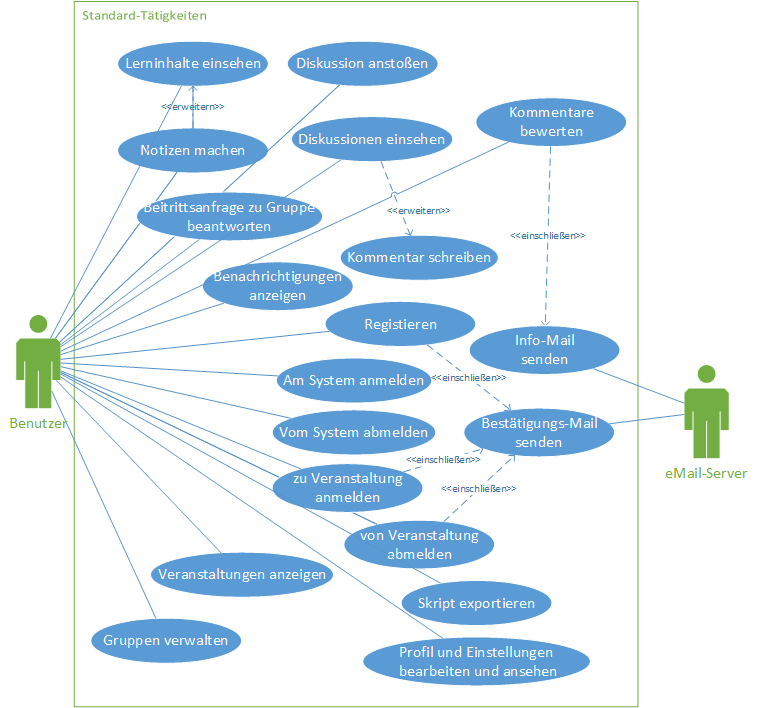
\includegraphics[width=\textwidth]{Bilder/Anwendungsfalldiagramme/Benutzer.png}
	\caption{Dies sind alle Aktionen die von einem Benutzer getätigt werden können.}
	\label{AwfBenutzer}
\end{figure}

\begin{figure}[H]
	\centering
	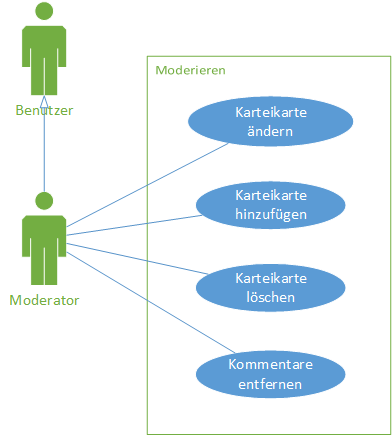
\includegraphics[height=10cm]{Bilder/Anwendungsfalldiagramme/Moderator.png}
	\caption{Der Moderator erbt alle Anwendungsfälle vom Benutzer. Er kann zusätzlich die Karteikarten und Diskussionen verwalten.}
	\label{AwfModerator}
\end{figure}

\begin{figure}[H]
	\centering
	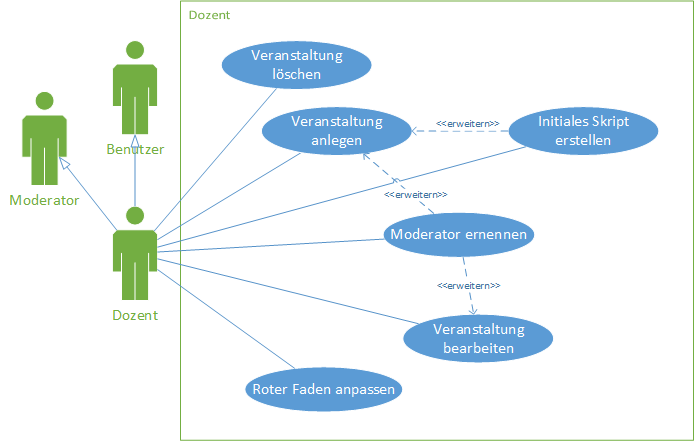
\includegraphics[width=\textwidth]{Bilder/Anwendungsfalldiagramme/Dozent.png}
	\caption{Der Dozent erbt alle Anwendungsfälle vom Benutzer und vom Moderator. Zusätzlich kann er Veranstaltungen verwalten.}
	\label{AwfDozent}
\end{figure}

\begin{figure}[H]
	\centering
	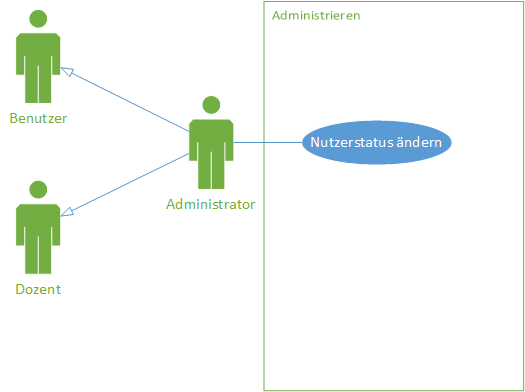
\includegraphics[width=10cm]{Bilder/Anwendungsfalldiagramme/Admin.png}
	\caption{Der Administrator erbt von allen Akteuren und hat somit alle Rechte. Er kann Nutzer in den Dozenten-Status erheben.}
	\label{AwfAdmin}
\end{figure}

\newpage

\subsubsection*{Anwendungsszenarien}
Alle Anwendungsfälle werden durch Sequenzdiagramme beschrieben. Diese Diagramme beschreiben einen beispielhaften Ablauf und die möglichen Alternativen einer Aktion auf. In den Sequenzdiagrammen werden die einzelnen Objekte durch eine viereckiges Kästchen dargestellt. Die Verbindungen zwischen den Objekten stellen die Interaktionen und die dazu bereitgestellten Informationen oder Daten des Systems dar. Die einzelnen Balken auf den Objekten stellen die Dauer der Operation oder des Funktionsaufrufes dar.

\begin{figure}[H]
	\centering
	\paragraph{Registrierung}
	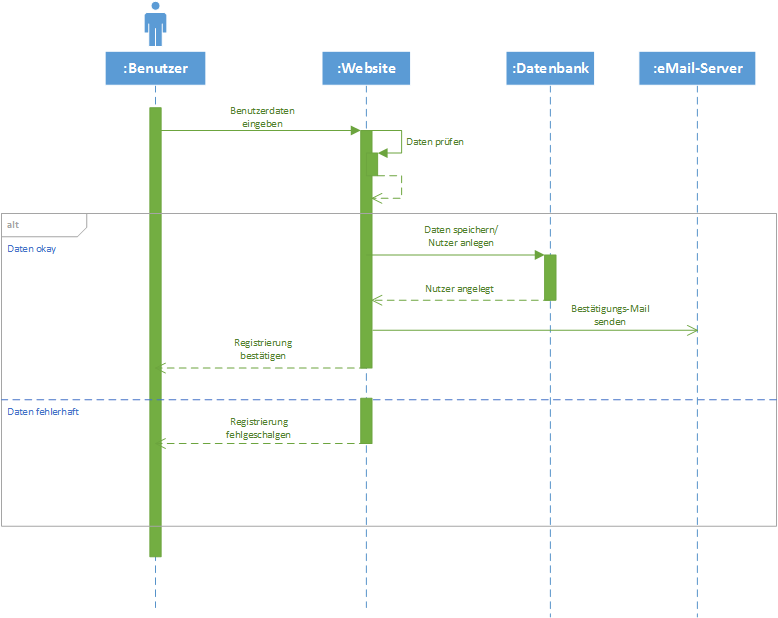
\includegraphics[width=\textwidth]{Bilder/Sequenzdiagramme/Registrieren.png}
	\caption{Die initiale Benutzerregistrierung im System.}
	\label{SzRegistrieren}
\end{figure}
\begin{figure}[H]
	\centering
	\paragraph{Profil bearbeiten}
	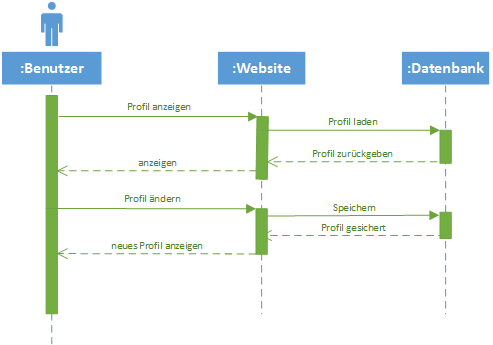
\includegraphics[width=\textwidth]{Bilder/Sequenzdiagramme/ProfilBearbeiten.png}
	\caption{Der Benutzer bearbeitet sein persönliches Profil.}
	\label{SzProfilBearbeiten}
\end{figure}
\begin{figure}[H]
	\centering
	\paragraph{Am System anmelden}
	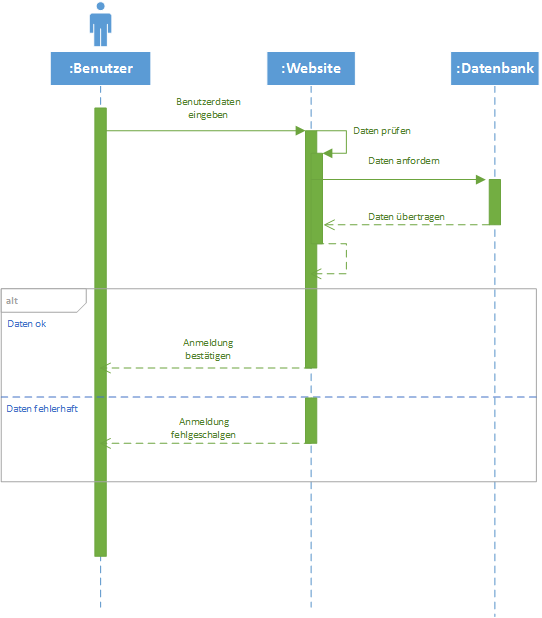
\includegraphics[width=\textwidth]{Bilder/Sequenzdiagramme/AmSystemAnmelden.png}
	\caption{Die Benutzeranmeldung am System.}
	\label{SzAmSystemAnmelden}
\end{figure}
\begin{figure}[H]
	\centering
	\paragraph{Vom System abmelden}\mbox{}\\
	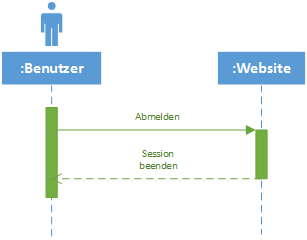
\includegraphics[width=10cm]{Bilder/Sequenzdiagramme/VomSystemAbmelden.png}
	\caption{Die Benutzerabmeldung}
	\label{SzVomSystemAbmelden}
\end{figure}
\begin{figure}[H]
	\centering
	\paragraph{Von einer Veranstaltung abmelden}
	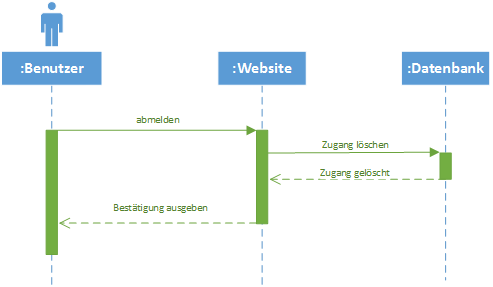
\includegraphics[width=\textwidth]{Bilder/Sequenzdiagramme/VonVeranstaltungAbmelden.png}
	\caption{Der Benutzer meldet sich von einer Veranstaltung ab.}
	\label{SzVonVeranstaltungAbmelden}
\end{figure}
\begin{figure}[H]
	\centering
	\paragraph{Zu einer Veranstaltung anmelden}
	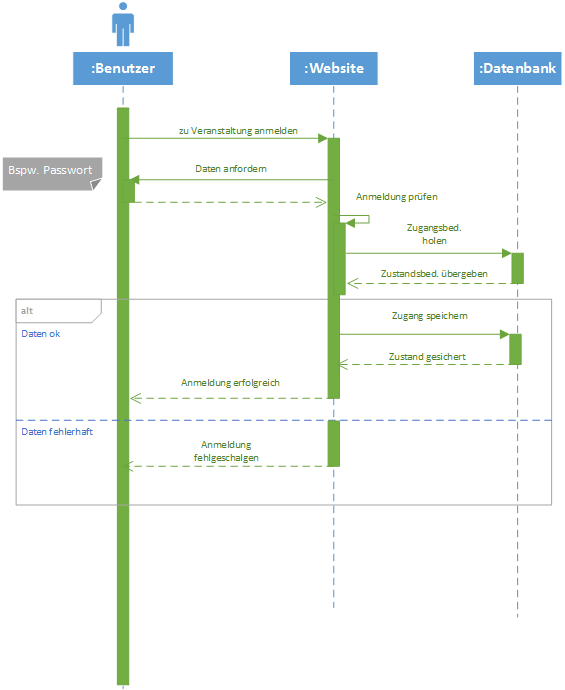
\includegraphics[width=\textwidth]{Bilder/Sequenzdiagramme/ZuVeranstaltungAnmelden.png}
	\caption{Die Anmeldung von einem Benutzer zu einer Veranstaltung.}
	\label{SzZuVeranstaltungAnmelden}
\end{figure}
\begin{figure}[H]
	\centering
	\paragraph{Veranstaltung anzeigen}
	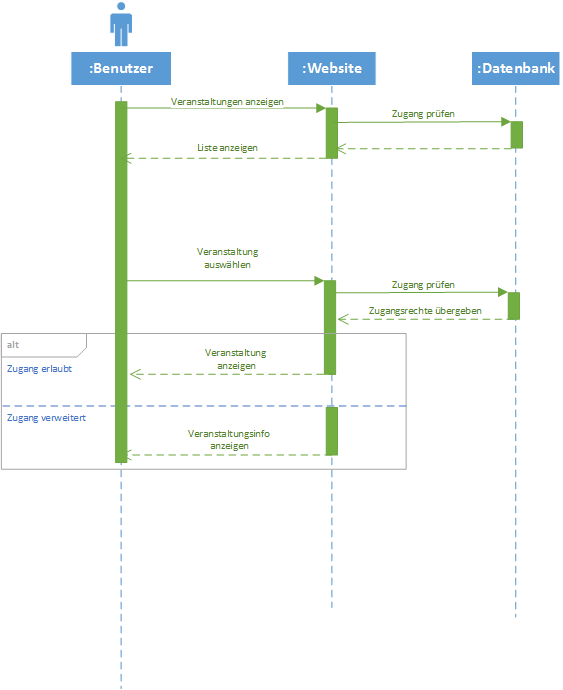
\includegraphics[width=\textwidth]{Bilder/Sequenzdiagramme/VeranstaltungAnzeigen.png}
	\caption{Der Benutzer zeigt sich alle bestehenden Veranstaltungen an.}
	\label{SzVeranstaltungenAnzeigen}
\end{figure}
\begin{figure}[H]
	\centering
	\paragraph{Eine neue Veranstaltung anlegen}
	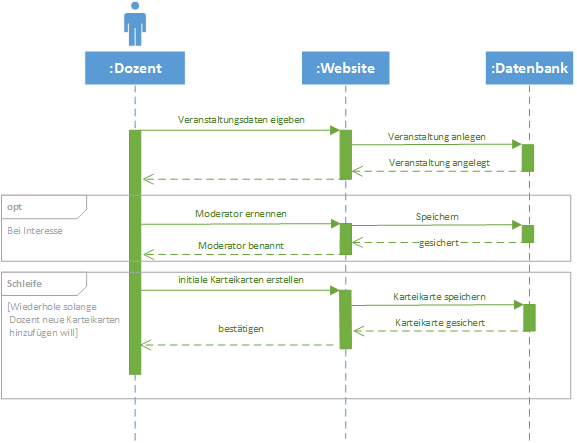
\includegraphics[width=\textwidth]{Bilder/Sequenzdiagramme/VeranstaltungAnlegen.png}
	\caption{Der Dozent erstellt eine neue Veranstaltung.}
	\label{SzVeranstaltungAnlegen}
\end{figure}
\begin{figure}[H]
	\centering
	\paragraph{Eine vorhandene Veranstaltung löschen}
	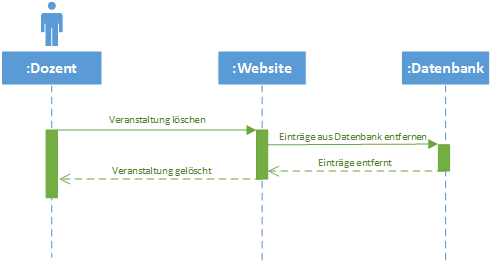
\includegraphics[width=\textwidth]{Bilder/Sequenzdiagramme/VeranstaltungLoeschen.png}
	\caption{Die vom dem Dozenten erstellte Veranstaltungen löschen.}
	\label{SzVeranstaltungLoeschen}
\end{figure}
\begin{figure}[H]
	\centering
	\paragraph{Veranstaltung bearbeiten}
	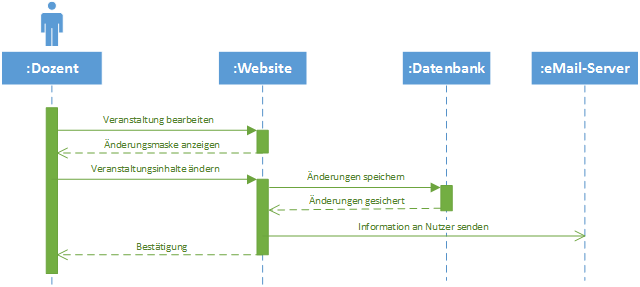
\includegraphics[width=\textwidth]{Bilder/Sequenzdiagramme/VeranstaltungBearbeiten.png}
	\caption{Der Dozent nimmt Änderungen an seiner Veranstaltungen vor.}
	\label{SzVeranstaltungBearbeiten}
\end{figure}
\begin{figure}[H]
	\centering
	\paragraph{Lerninhalt einsehen}
	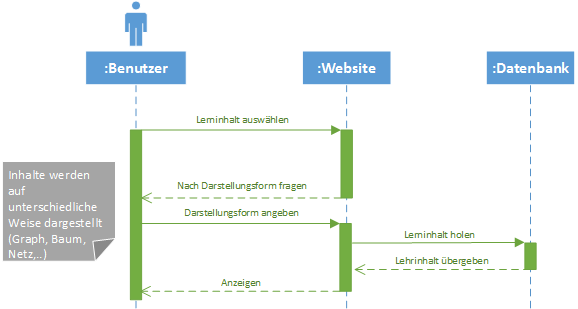
\includegraphics[width=\textwidth]{Bilder/Sequenzdiagramme/LehrinhalteEinsehen.png}
	\caption{Der Benutzer zeigt sich eine Diskussion zu einer Karteikarte an.}
	\label{SzLerninhaltEinsehen}
\end{figure}
\begin{figure}[H]
	\centering
	\paragraph{Roter Faden bearbeiten}
	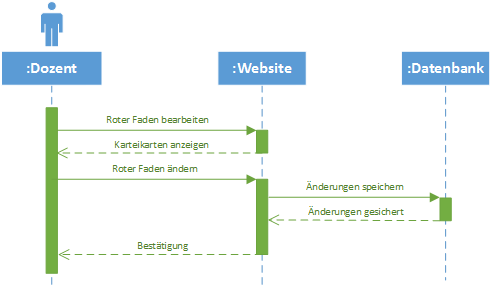
\includegraphics[width=\textwidth]{Bilder/Sequenzdiagramme/RoterFadenBearbeiten.png}
	\caption{Der Dozent nimmt Änderungen am roten Faden vor.}
	\label{SzRoterFaden}
\end{figure}
\begin{figure}[H]
	\centering
	\paragraph{Notizen machen}
	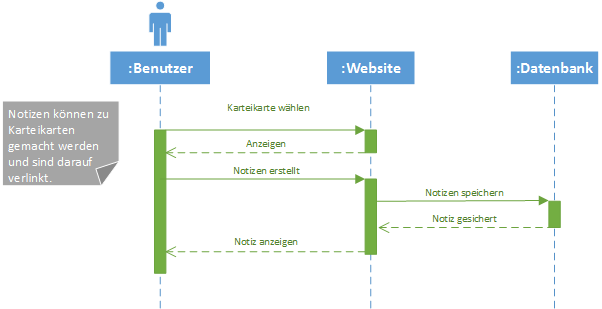
\includegraphics[width=\textwidth]{Bilder/Sequenzdiagramme/NotizenMachen.png}
	\caption{Der Benutzer legt eine Notiz zu einer Karteikarte an.}
	\label{SzNotizenMachen}
\end{figure}
\begin{figure}[H]
	\centering
	\paragraph{Skript exportieren}
	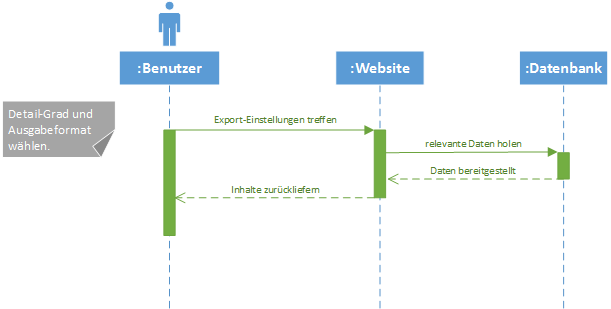
\includegraphics[width=\textwidth]{Bilder/Sequenzdiagramme/SkriptExportieren.png}
	\caption{Der Benutzer exportiert das Skript.}
	\label{SzSkriptExportieren}
\end{figure}
\begin{figure}[H]
	\centering
	\paragraph{Diskussion beginnen}
	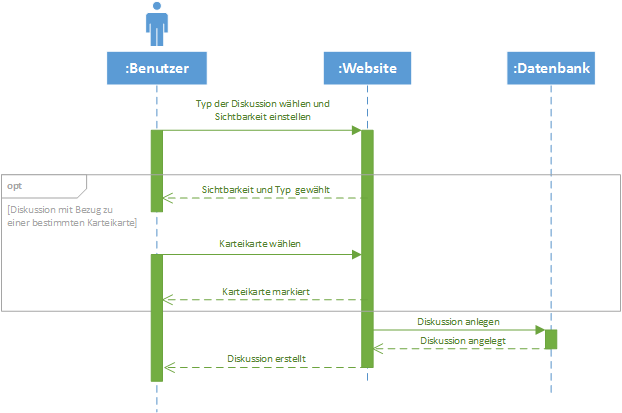
\includegraphics[width=\textwidth]{Bilder/Sequenzdiagramme/DiskussionAnstossen.png}
	\caption{Der Benutzer stößt eine Diskussion zu einer Karteikarte an.}
	\label{SzDiskussionAnstossen}
\end{figure}
\begin{figure}[H]
	\centering
	\paragraph{Diskussion einsehen}
	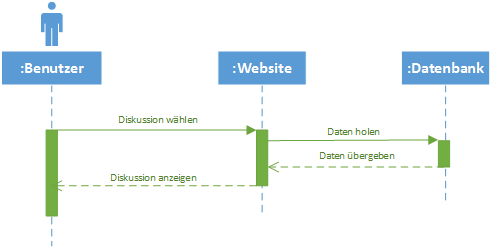
\includegraphics[width=\textwidth]{Bilder/Sequenzdiagramme/DiskussionEinsehen.png}
	\caption{Der Benutzer lässt sich eine Diskussion zu einer Karteikarte anzeigen.}
	\label{SzDiskussionEinsehen}
\end{figure}
\begin{figure}[H]
	\centering
	\paragraph{Kommentar schreiben}
	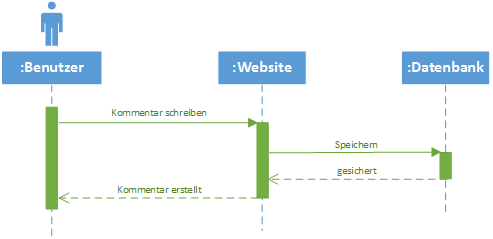
\includegraphics[width=\textwidth]{Bilder/Sequenzdiagramme/KommentarSchreiben.png}
	\caption{Der Nutzer hinterlässt einen Kommentar zu einer Diskussion.}
	\label{SzKommentarSchreiben}
\end{figure}
\begin{figure}[H]
	\centering
	\paragraph{Kommentare bewerten}
	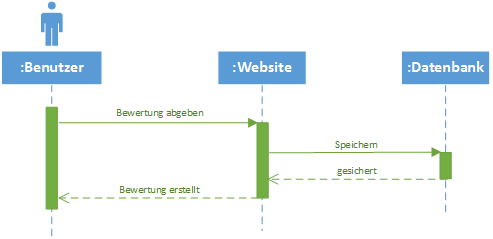
\includegraphics[width=\textwidth]{Bilder/Sequenzdiagramme/KommentarBewerten.png}
	\caption{Der Nutzer bewertet einen Kommentar in einer Diskussion.}
	\label{SzKommentareBewerten}
\end{figure}
\begin{figure}[H]
	\centering
	\paragraph{Kommentare löschen}
	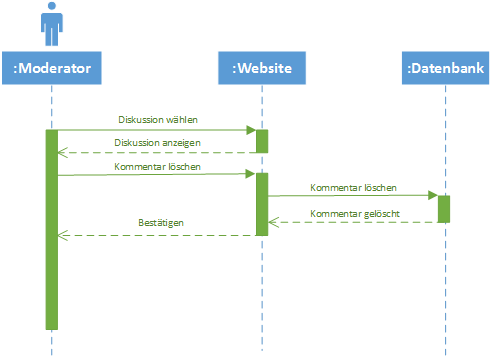
\includegraphics[width=\textwidth]{Bilder/Sequenzdiagramme/KommentarLoeschen.png}
	\caption{Der Moderator löscht nicht relevante Kommentare.}
	\label{SzKommentarLoeschen}
\end{figure}
\begin{figure}[H]
	\centering
	\paragraph{Karteikarte hinzufügen}
	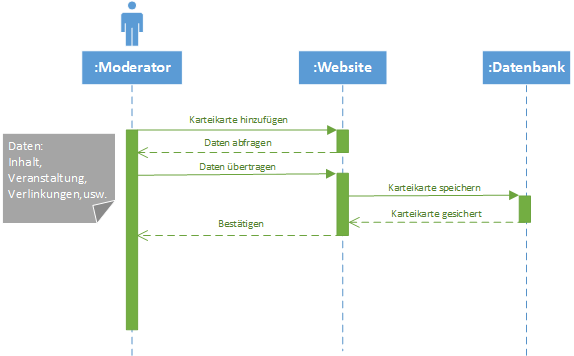
\includegraphics[width=\textwidth]{Bilder/Sequenzdiagramme/KarteikarteHinzufuegen.png}
	\caption{Der Moderator fügt eine neue Karteikarte hinzu.}
	\label{SzKarteikarteHinzufuegen}
\end{figure}
\begin{figure}[H]
	\centering
	\paragraph{Karteikarte ändern}
	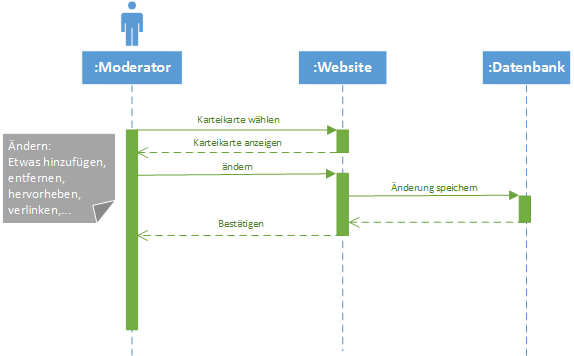
\includegraphics[width=\textwidth]{Bilder/Sequenzdiagramme/KarteikarteAendern.png}
	\caption{Der Moderator ändert eine Karteikarte.}
	\label{SzKarteikarteAendern}
\end{figure}
\begin{figure}[H]
	\centering
	\paragraph{Karteikarte löschen}
	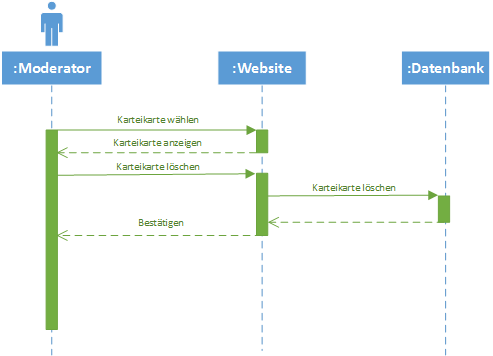
\includegraphics[width=\textwidth]{Bilder/Sequenzdiagramme/KarteikarteLoeschen.png}
	\caption{Der Moderator löscht eine Karteikarte.}
	\label{SzKarteikarteLoeschen}
\end{figure}
\begin{figure}[H]
	\centering
	\paragraph{Gruppe verwalten}
	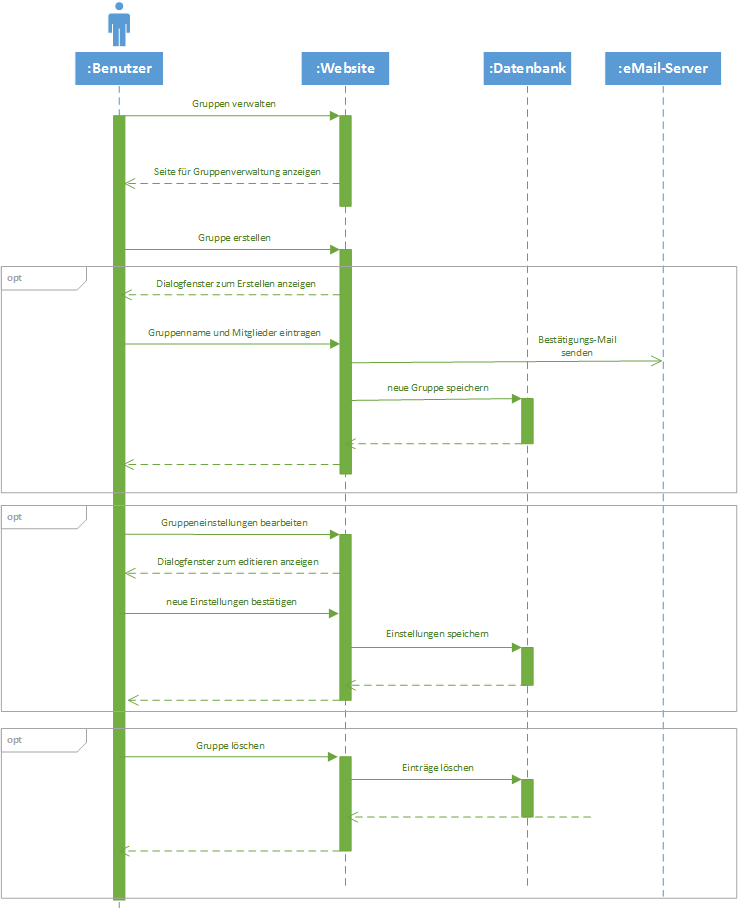
\includegraphics[width=\textwidth]{Bilder/Sequenzdiagramme/GruppenVerwalten.png}
	\caption{Der Benutzer verwaltet die Gruppen.}
	\label{SzGruppenVerwalten}
\end{figure}
\begin{figure}[H]
	\centering
	\paragraph{Beitrittsanfrage zu Gruppe beantworten}
	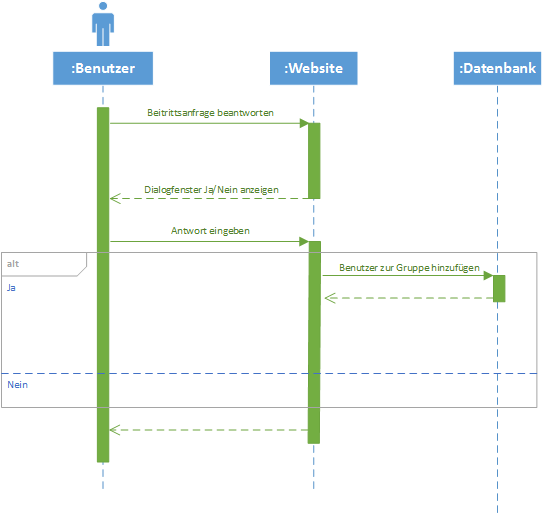
\includegraphics[width=\textwidth]{Bilder/Sequenzdiagramme/BeitrittsanfrageZuGruppe.png}
	\caption{Der Benutzer beantwortet Beitrittsanfragen zu Gruppen.}
	\label{SzBeitrittsanfrageZuGruppe}
\end{figure}
\begin{figure}[H]
	\centering
	\paragraph{Benachrichtigungen anzeigen}
	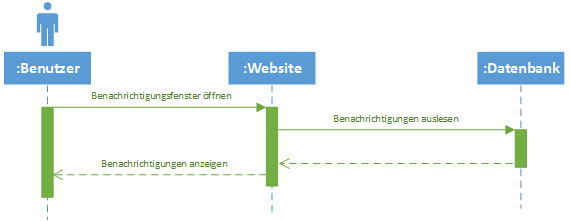
\includegraphics[width=\textwidth]{Bilder/Sequenzdiagramme/BenachrichtigungenAnzeigen.png}
	\caption{Der Benutzer zeigt sich seine Benachrichtigungen an.}
	\label{SzBenachrichtigungen}
\end{figure}
\begin{figure}[H]
	\centering
	\paragraph{Nutzerstatus ändern}
	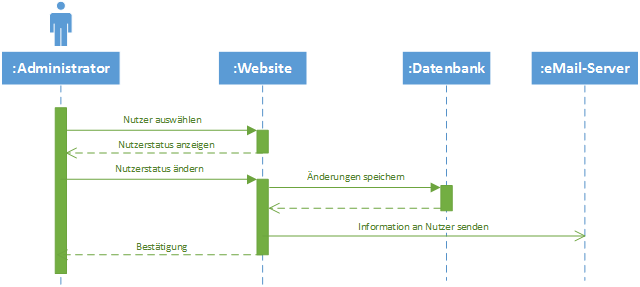
\includegraphics[width=\textwidth]{Bilder/Sequenzdiagramme/NutzerstatusAendern.png}
	\caption{Der Administrator ändert die Profildaten eines Benutzers.}
	\label{SzNutzerstatusAendern}
\end{figure}

\begin{figure}[H]
	\centering
	\paragraph{Mail versenden}\mbox{}\\
	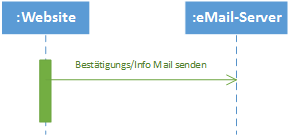
\includegraphics[width=10cm]{Bilder/Sequenzdiagramme/MailVersenden.png}
	\caption{Das System sendet eine Mail an den Benutzer.}
	\label{SzMailVersenden}
\end{figure}


\subsection{Funktionale Systemanforderungen}
Hier werden alle Systemaufgaben, die dazugehörigen Teilnehmer und jeweils eine kurze Beschreibung aufgelistet. Außerdem wird jede Anforderung mit einer Markierung (von nicht sehr von Bedeutung [-2]  bis [2] sehr wichtig) versehen, die darlegt, wie wichtig diese Anforderung ist.

\paragraph{Benutzer - Anwendungsfall "Registrieren" (2)}\mbox{}\\
\textbf{Eingabe der Daten}\\
\begin{tabular}{l| p{12cm}}
\hline 
Beteiligt & Anonym, System \\ 
Beschreibung & Eine anonyme Person kann ihre Zugangsdaten bei der Registrierung eingeben. Mit diesen Daten wird dann ein neuer Benutzer im System angemeldet.\\ 
\end{tabular}\\

\textbf{Registrierung bestätigen}\\
\begin{tabular}{l|p{12cm}}
\hline 
Beteiligt    & Benutzer, System, eMail-Server \\ 
Beschreibung & Die erfolgreiche Anmeldung wird dem Benutzer  \\
 			 & per Dialog und zusätzlich per Mail bestätigt. \\ 
\end{tabular} 

\newpage
\paragraph{Benutzer - Anwendungsfall \glqq Am System anmelden\grqq (2)}\mbox{}

\textbf{Eingabe der Zugangsdaten}\\
\begin{tabular}{l|p{12cm}}
\hline 
Beteiligt & Benutzer, System \\ 
Beschreibung & Der Nutzer gibt seine Zugangsdaten ein. Wenn die Anmeldung erfolgreich war wird der Nutzer am System angemeldet. Bei inrorrekten Zugangsdaten erscheint eine Fehlermeldung. \\ 
\end{tabular}\\


\textbf{Anmeldung bestätigen}\\
\begin{tabular}{l|p{12cm}}
\hline 
Beteiligt & Benutzer, System \\ 
Beschreibung & Das System bestätigt dem Nutzer die Anmeldung. \\ 
\end{tabular}\\\\


\paragraph{Benutzer - Anwendungsfall \glqq Vom System abmelden\grqq (2)}\mbox{}

\textbf{Abmelden}\\
\begin{tabular}{l|p{12cm}}
\hline 
Beteiligt & Benutzer, System \\ 
Beschreibung & Bei der Abmeldung vom System wird die Session vom Benutzer beendet.\\ 
\end{tabular}\\

\textbf{Abmeldung bestätigen}\\
\begin{tabular}{l|p{12cm}}
\hline 
Beteiligt & Benutzer, System \\ 
Beschreibung &  Das System zeigt an, dass das Abmelden erfolgreich war. \\ 
\end{tabular}\\\\



\paragraph{Benutzer - Anwendungsfall \glqq Veranstaltungen anzeigen\grqq (2)}\mbox{}

\textbf{Alle Veranstaltungen anzeigen}\\
\begin{tabular}{l|p{12cm}}
\hline 
Beteiligt & Benutzer, System  \\ 
Beschreibung & Das System zeigt dem Benutzer alle verfügbaren Veranstaltungen an. \\ 
\end{tabular}\\ 

\textbf{Veranstaltungen auswählen und anzeigen}\\
\begin{tabular}{l|p{12cm}}
\hline 
Beteiligt & Benutzer, System \\ 
Beschreibung & Das System zeigt dem Benutzer alle Veranstaltung an, an denen er nicht angemeldet ist. Ist der Benutzer schon zu einer Veranstaltung angemeldet, wird ihm direkt die eigentliche Veranstaltungsseite angezeigt. \\ 
\end{tabular} \\\\

\newpage

\paragraph{Benutzer - Anwendungsfall \glqq Zu Veranstaltung anmelden \grqq (2)}\mbox{}

\textbf{Zu Veranstaltung anmelden}\\
\begin{tabular}{l|p{12cm}}
\hline 
Beteiligt & Benutzer, System \\ 
Beschreibung & Nachdem der Benutzer die Zugangsdaten zur Veranstaltung korrekt angegeben hat, wird die Zugangsberechtigung vom System übernommen und der Benutzer wird zur Veranstaltungsseite weitergeleitet. Andernfalls wird ihm eine Fehlermeldung angezeigt.\\ 
\end{tabular}\\\\


\paragraph{Benutzer - Anwendungsfall \glqq Von Veranstaltung abmelden\grqq (0)}\mbox{}

\textbf{Von Veranstaltung abmelden}\\
\begin{tabular}{l|p{12cm}}
\hline 
Beteiligt & Benutzer, System \\ 
Beschreibung & Das System meldet den Benutzer vom System ab und zeigt Ihm an ob der Vorgang erfolgreich war. \\ 
\end{tabular}\\\\


\paragraph{Benutzer - Anwendungsfall \glqq Skript exportieren\grqq (-1)}\mbox{}

\textbf{Exportseite anzeigen und Skript wählen}\\
\begin{tabular}{l|p{12cm}}
\hline 
Beteiligt & Benutzer, System \\ 
Beschreibung & Der Nutzer bekommt eine Exportoberfläche angezeigt, auf der er den zu exportierenden Lernstoff wählen kann. \\ 
\end{tabular}\\

\textbf{Exporteinstellungen treffen}\\
\begin{tabular}{l|p{12cm}}
\hline 
Beteiligt & Benutzer, System \\ 
Beschreibung & Der Benutzer hat die Möglichkeit die Export-Einstellungen festzulegen. \\ 
\end{tabular}\\

\textbf{Skript exportieren}\\
\begin{tabular}{l|p{12cm}}
\hline 
Beteiligt & Benutzer, System \\ 
Beschreibung & Das System generiert das Dokument und bietet es dem Nutzer zum Download an. \\ 
\end{tabular}\\\\


\paragraph{Benutzer - Anwendungsfall \glqq Profil und Einstellungen bearbeiten und ansehen\grqq  (2)}\mbox{}

\textbf{Profil anzeigen}\\
\begin{tabular}{l|p{12cm}}
\hline 
Beteiligt & Benutzer, System \\ 
Beschreibung & Der Nutzer kann sein eigenes Profil oder das anderer Benutzer einsehen. \\ 
\end{tabular}\\

\textbf{Profil bearbeiten}\\
\begin{tabular}{l|p{12cm}}
\hline 
Beteiligt & Benutzer, System \\ 
Beschreibung & Jeder Nutzer kann sein eigenes Profil bearbeiten. \\ 
\end{tabular}\\ 

\textbf{Einstellungen bearbeiten}\\
\begin{tabular}{l|p{12cm}}
\hline 
Beteiligt & Benutzer, System \\ 
Beschreibung & Das System bietet dem Nutzer eine Oberfläche um sämtliche Einstellungen festzulegen. \\ 
\end{tabular}\\

\textbf{Einstellungen- und Profil-Änderungen speichern}\\
\begin{tabular}{l|p{12cm}}
\hline 
Beteiligt &  Benutzer, System \\ 
Beschreibung & Das System bestätigt dem Benutzer die erfolgreiche Änderung oder gibt eine Fehlermeldung aus. \\ 
\end{tabular}\\\


\paragraph{Benutzer - Anwendungsfall \glqq Diskussion anstoßen\grqq (1)}\mbox{}

\textbf{Neue Diskussion erstellen}\\
\begin{tabular}{l|p{12cm}}
\hline 
Beteiligt & Benutzer, System \\ 
Beschreibung & Jeder Nutzer kann eine neue Diskussion zu einer Karteikarte erstellen. \\ 
\end{tabular}\\

\textbf{Sichtbarkeit einstellen}\\
\begin{tabular}{l|p{12cm}}
\hline 
Beteiligt & Benutzer, System \\ 
Beschreibung & Der Nutzer kann beim Erstellen die Sichtbarkeit der Diskussion einstellen (Öffentlich ersichtlich, nur in der Veranstaltung, nur in der Gruppe). \\ 
\end{tabular}\\\\


\paragraph{Benutzer - Anwendungsfall \glqq Kommentare machen\grqq (1)}\mbox{}

\textbf{Kommentar hinzufügen}\\
\begin{tabular}{l|p{12cm}}
\hline 
Beteiligt & Benutzer, System \\ 
Beschreibung & Jeder Benutzer muss, wenn er die notwendigen Rechte besitzt, Kommentare zu einer Diskussion hinzufügen. \\ 
\end{tabular}\\\\ 


\paragraph{Benutzer - Anwendungsfall \glqq Notizen machen\grqq (1)}\mbox{}

\textbf{Notizen hinzufügen}\\
\begin{tabular}{l|p{12cm}}
\hline 
Beteiligt & Benutzer, System \\ 
Beschreibung & Jeder Benutzer muss sich zu einer Karteikarte Notizen machen. \\ 
\end{tabular}\\\\


\paragraph{Benutzer - Anwendungsfall \glqq Kommentare bewerten\grqq (-1)}\mbox{}

\textbf{Kommentar bewerten}\\
\begin{tabular}{l|p{12cm}}
\hline 
Beteiligt & Benutzer, Moderator, System \\ 
Beschreibung & Jeder Benutzer kann, wenn er die notwendigen Rechte(Sichtbarkeit) hat, bewerten. Ein Moderator kann alle Kommentare  bewerten egal welche Sichtbarkeit dieser besitzt. \\ 
\end{tabular}\\\\


\paragraph{Benutzer - Anwendungsfall \glqq Gruppen verwalten\grqq (-2)}\mbox{}

\textbf{Gruppe erstellen}\\
\begin{tabular}{l|p{12cm}}
\hline 
Beteiligt & Benutzer, System \\ 
Beschreibung & Jeder Benutzer besitzt Zugriff auf eine Gruppenerstellungsmaske, um eine neue Gruppe hinzufügen. \\ 
\end{tabular}\\

\textbf{Gruppe löschen}\\
\begin{tabular}{l|p{12cm}}
\hline 
Beteiligt & Benutzer, System \\ 
Beschreibung & Jeder Benutzer besitzt Zugriff auf ein Menü, um seine selbst erstellten Gruppen zu löschen. \\ 
\end{tabular}\\

\textbf{Gruppe editieren}\\
\begin{tabular}{l|p{12cm}}
\hline 
Beteiligt & Benutzer, System \\ 
Beschreibung & Jeder Benutzer hat die Möglichkeit, seine selbst erstellten Gruppen zu editieren, indem er bspw. neue Mitglieder hinzufügt. \\ 
\end{tabular}\\\\


\paragraph{Benutzer - Anwendungsfall \glqq Benachrichtigungen anzeigen\grqq  (1)}\mbox{}

\textbf{Benachrichtigungen anzeigen}\\
\begin{tabular}{l|p{12cm}}
\hline 
Beteiligt & Benutzer, System \\ 
Beschreibung & Jedem Benutzer werden immer aktuelle Informationen wie eine Beitrittsanfrage zu einer Gruppe, oder neue Kommentare angezeigt. \\ 
\end{tabular}\\\\
 


\paragraph{Benutzer - Anwendungsfall \glqq Lerninhalte anzeigen\grqq  (2)}\mbox{}

\textbf{Lerninhalte anzeigen}\\
\begin{tabular}{l|p{12cm}}
\hline 
Beteiligt & Benutzer, System  \\ 
Beschreibung & Jedem Benutzer werden die Lerninhalte zu einer Veranstaltung angezeigt, zu der er angemeldet ist. \\ 
\end{tabular}\\


\paragraph{Benutzer - Anwendungsfall \glqq Beitrittsanfrage zu Gruppe beantworten\grqq (-2)}\mbox{}

{\textbf{Beitrittsanfragen beantworten}\\
\begin{tabular}{l|p{12cm}}
\hline 
Beteiligt & Benutzer, Moderator, System \\ 
Beschreibung & Jeder Benutzer kann über eine Oberfläche ausstehende Beitrittsanfragen annehmen oder ablehnen. \\ 
\end{tabular}\\\\


\paragraph{Dozent - Anwendungsfall \glqq Veranstaltung anlegen\grqq (2)}\mbox{}

\textbf{Veranstaltungsdaten eingeben}\\
\begin{tabular}{l|p{12cm}}
\hline 
Beteiligt & Dozent, System \\ 
Beschreibung & Es gibt eine Oberfläche, wo der Dozent die Veranstaltungsdaten(Name, Beschreibung, Zugangspasswort,..) eingeben kann. Daraufhin wird eine neue Veranstaltung im System angelegt. Siehe auch Anwendungsfall \glqq Initiales Skript importieren \grqq . \\ 
\end{tabular} \\\\


\paragraph{Dozent - Anwendungsfall \glqq Moderator ernennen\grqq (2)}\mbox{}

\textbf{Moderator ernennen}\\
\begin{tabular}{l|p{12cm}}
\hline 
Beteiligt & Dozent, System \\ 
Beschreibung & Der Dozent kann für seine Veranstaltungen Moderatoren angeben. \\ 
\end{tabular}\\\\


\paragraph{Dozent - Anwendungsfall \glqq Initiales Skript erstellen\grqq (1)}\mbox{}

\textbf{Importseite anzeigen und Skript hochladen}\\
\begin{tabular}{l|p{12cm}}
\hline 
Beteiligt & Dozent, System \\ 
Beschreibung & Der Dozent bekommt eine Importoberfläche angezeigt und lädt ein Skript hoch. Nachdem der Dozent die Import-Einstellungen angegeben hat, konvertiert das System dieses Skript in die Karteikarten-Repräsentation, erstellt den initialen roten Faden und bietet die Möglichkeit zusätzliche Verlinkungen einzufügen. \\ 
\end{tabular}\\\\

\newpage

\paragraph{Dozent - Anwendungsfall \glqq Veranstaltung bearbeiten\grqq (0)}\mbox{}

\textbf{Veranstaltung bearbetien}\\
\begin{tabular}{l|p{12cm}}
\hline 
Beteiligt & Dozent, System \\ 
Beschreibung & Der Dozent kann seine eigenen Veranstaltungen bearbeiten, indem er neue Moderatoren hinzufügt, andere löscht, optionale Features ein oder aus schaltet oder die Veranstaltungsbeschreibung ändert. \\ 
\end{tabular}\\\\


\paragraph{Dozent - Anwendungsfall \glqq Roter Faden anpassen\grqq (2)}\mbox{}

\textbf{Roter Faden anpassen}\\
\begin{tabular}{l|p{12cm}}
\hline 
Beteiligt & Dozent, System \\ 
Beschreibung & Der Dozent kann den initialen roten Faden anpassen, indem er diesen Menüpunkt einfach bei der entsprechenden Veranstaltung wählt. Dann werden ihm die Karteikarten, die den roten Faden bilden als Liste angezeigt. Jetzt kann er andere Karteikarten einfügen, bestehende entfernen oder umsortieren. \\ 
\end{tabular}\\\\


\paragraph{Moderator - Anwendungsfall \glqq Karteikarte hinzufügen\grqq (2)}\mbox{}

\textbf{Karteikarte hinzufügen}\\
\begin{tabular}{l|p{12cm}}
\hline 
Beteiligt & Moderator, System \\ 
Beschreibung & Der Moderator kann Karteikarten zum bestehenden Lernstoff hinzufügen. Hierbei muss er das Verweisziel angeben und Attribute setzen. \\ 
\end{tabular}\\\\

\paragraph{Moderator - Anwendungsfall \glqq Karteikarte ändern\grqq (2)}\mbox{}

\textbf{Karteikarte ändern}\\
\begin{tabular}{l|p{12cm}}
\hline 
Beteiligt & Moderator, System \\ 
Beschreibung & Der Moderator muss Änderungen der Karteikarten vornehmen können. \\ 
\end{tabular}\\\\

\newpage

\paragraph{Moderator - Anwendungsfall \glqq Karteikarte entfernen\grqq (2)}\mbox{}

\textbf{Karteikarte entfernen}\\
\begin{tabular}{l|p{12cm}}
\hline 
Beteiligt & Moderator, System \\ 
Beschreibung & Der Moderator soll Karteikarten entfernen können. \\ 
\end{tabular}\\\\


\paragraph{Moderator - Anwendungsfall \glqq Kommentare entfernen\grqq (2)}\mbox{}

\textbf{Karteikarte entfernen}\\
\begin{tabular}{l|p{12cm}}
\hline 
Beteiligt & Moderator, System \\ 
Beschreibung & Der Moderator muss Kommentare entfernen können. \\ 
\end{tabular}\\\\

\paragraph{Administrator - Anwendungsfall \glqq Nutzerstatus ändern\grqq (2)}\mbox{}

\textbf{Nutzerstatus ändern}\\
\begin{tabular}{l|p{12cm}}
\hline 
Beteiligt & Administrator, System \\ 
Beschreibung & Der Administrator kann Benutzer in den Dozentenstatus erheben. Das heißt, dass sich Dozenten zu Beginn als Studenten im System registrieren müssen. \\ 
\end{tabular}\\\\ 

\begin{landscape}
\section{Softwarspezifikation}
\subsection{Systemschnittstellen}
In diesem Kapitel werden die Dialoge und ihr Zusammenhang dargestellt. Durch die Pfeile ist dargestellt, welche Dialogübergänge möglich sind. Auf den Pfeilen ist die Interaktion beschrieben die dafür notwendig ist. Beispielweise der Klick auf einen Link oder auf einen Button. Zusammengehörige Dialoge sind durch grüne Boxen gruppiert. Die Lernumgebung ist als hierarchischer Dialog aufgebaut. Die Dialoge innerhalb des Dialogs \glqq Lernumgebung anzeigen\grqq sind Teildialoge. Sie existieren  nicht als eigene Oberfläche. Nun wird zuerst eine Übersicht über die Dialoge dargestellt. Danach wird jeder Teil noch einmal vergrößert dargestellt.

\begin{figure}[H]
	\centering
	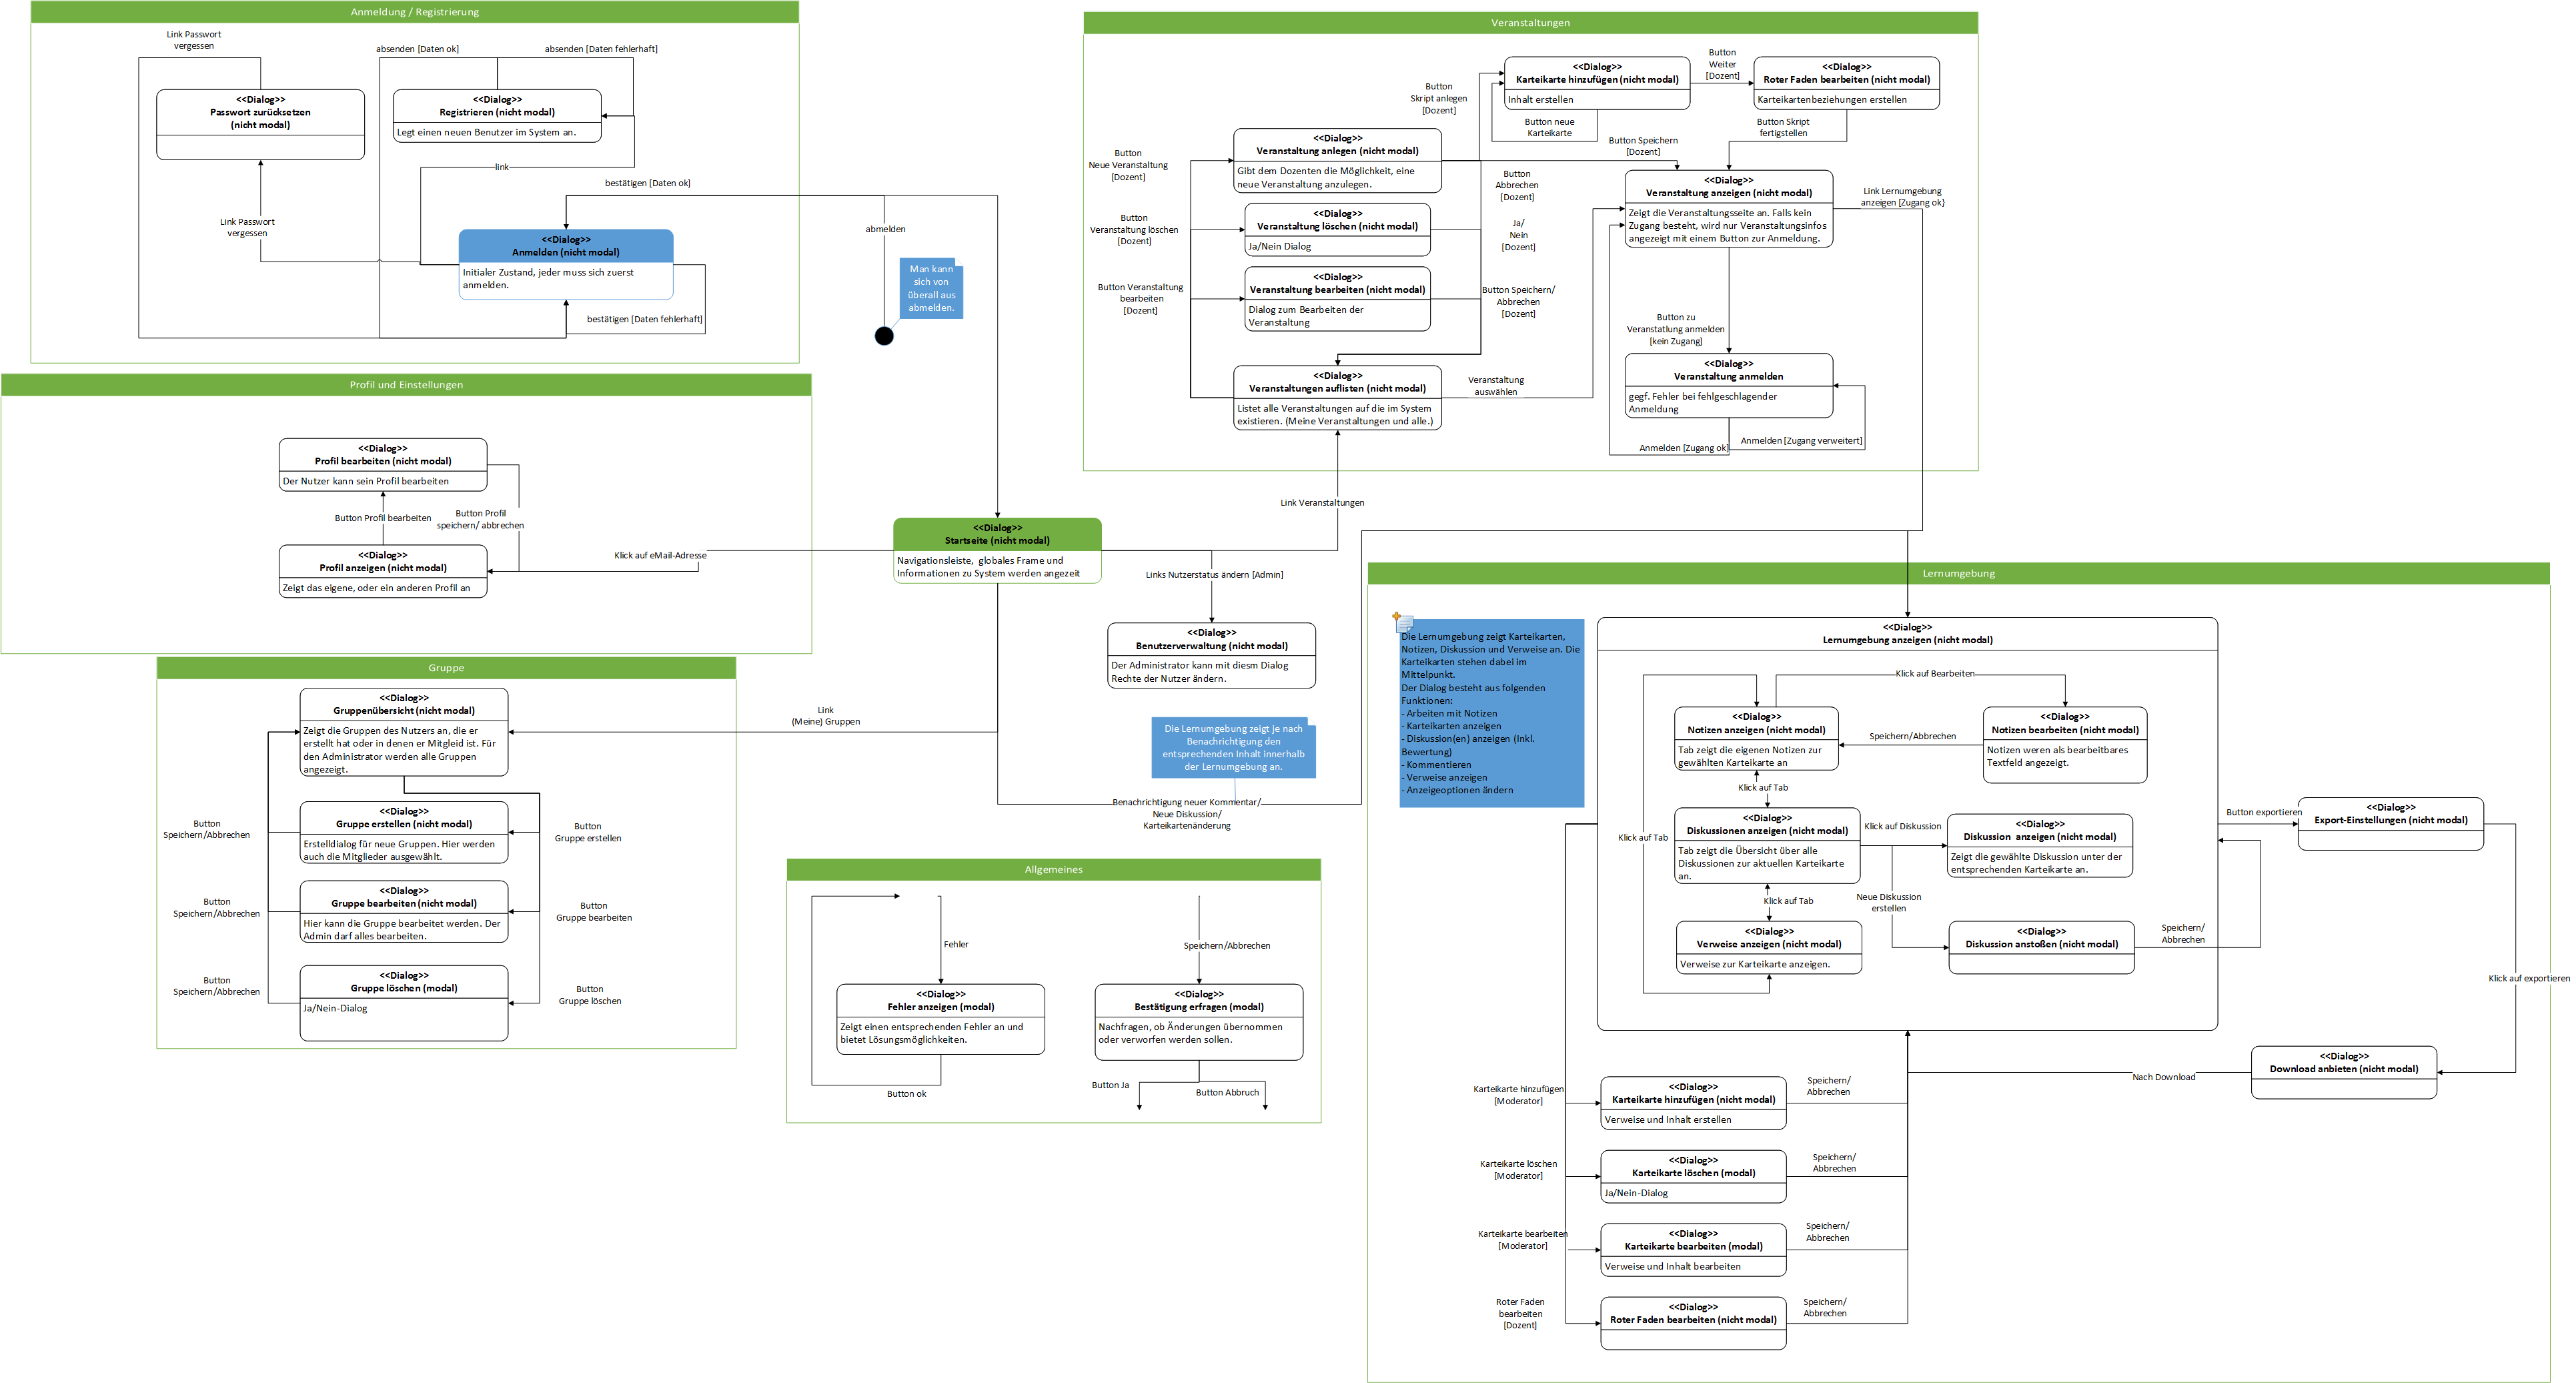
\includegraphics[width=18cm]{Bilder/Mockups/DSDGesamt.png}
	\caption{Überblick über Dialogstrukturdiagramm}
	\label{Dialogstrukturdiagramm}
\end{figure}

\begin{figure}[H]
	\centering
	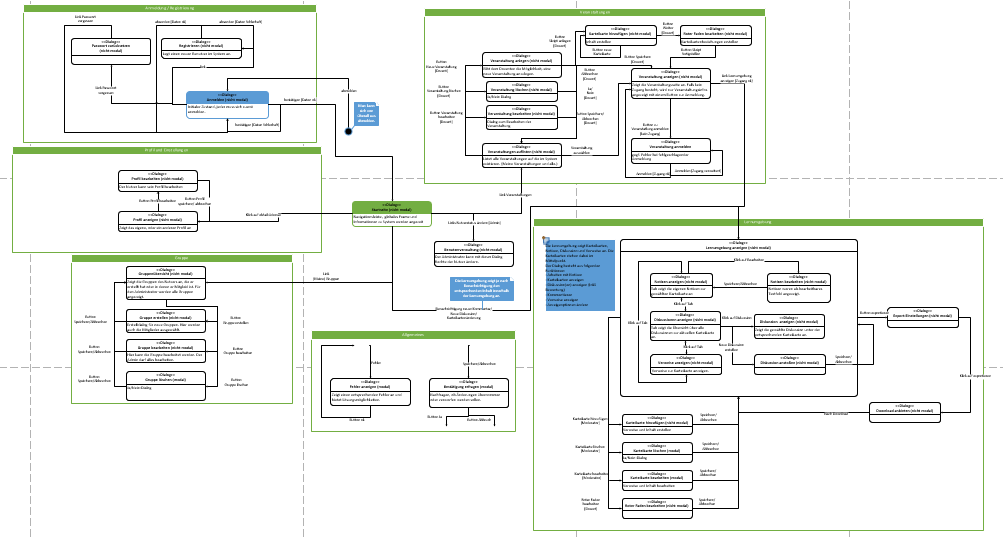
\includegraphics[width=25cm]{Bilder/Mockups/DSDGesamtuebersicht.png}
	\caption{Kompaktere Zusammenfassung}
	\label{DialogstrukturdiagrammZusammenfassung}
\end{figure}
\begin{figure}[H]
	\centering
	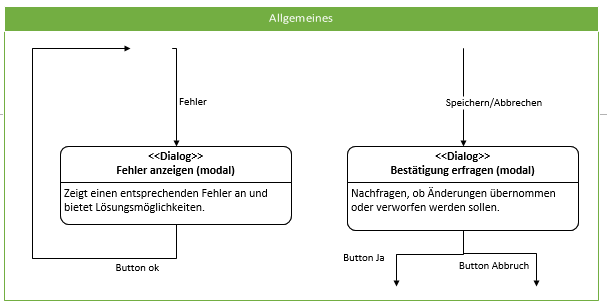
\includegraphics[width=20cm]{Bilder/Mockups/DSDAllgemeines.png}
	\caption{Allgemeine Bestätigungs- und Fehlerdialoge}
	\label{DSDAllgemeines}
\end{figure}

\begin{figure}[H]
	\centering
	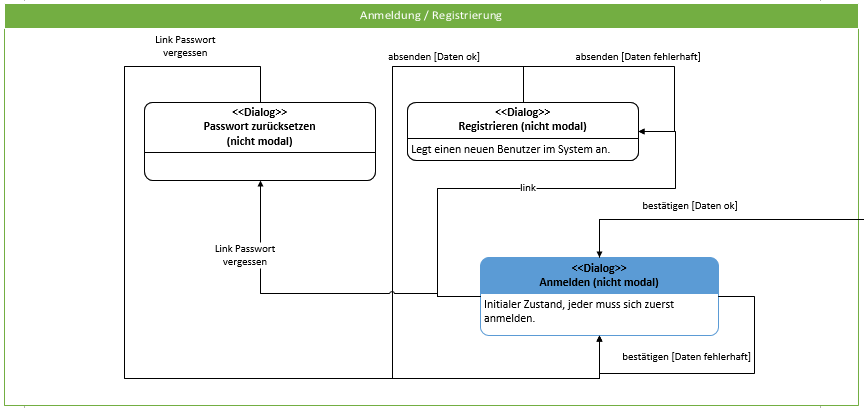
\includegraphics[width=20cm]{Bilder/Mockups/DSDAnmeldungRegistierung.png}
	\caption{Anmeldung und Registrierung}
	\label{DSDAnmeldungRegistierung}
\end{figure}

\begin{figure}[H]
	\centering
	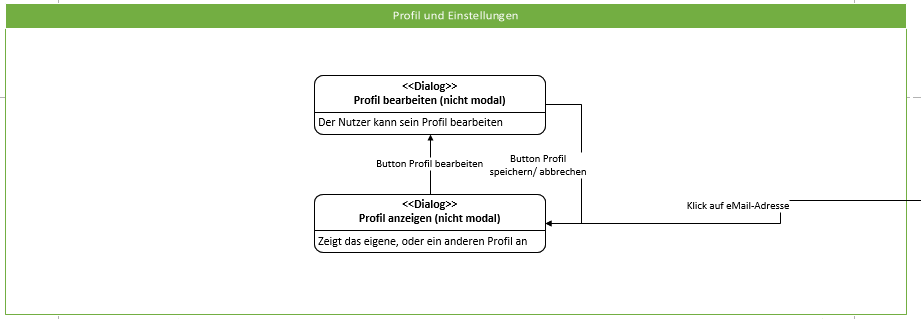
\includegraphics[width=23cm]{Bilder/Mockups/DSDProfilUndEinstellungen.png}
	\caption{Benutzer-Profil}
	\label{DSDProfilUndEinstellungen}
\end{figure}

\begin{figure}[H]
	\centering
	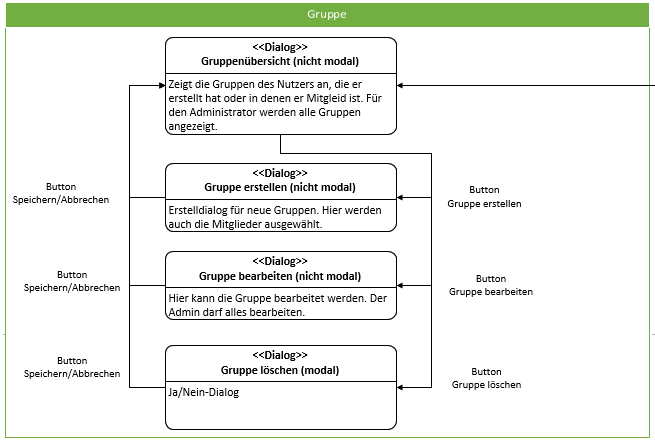
\includegraphics[width=20cm]{Bilder/Mockups/DSDGruppen.png}
	\caption{Gruppenübersicht und -verwaltung}
	\label{DSDGruppen}
\end{figure}

\begin{figure}[H]
	\centering
	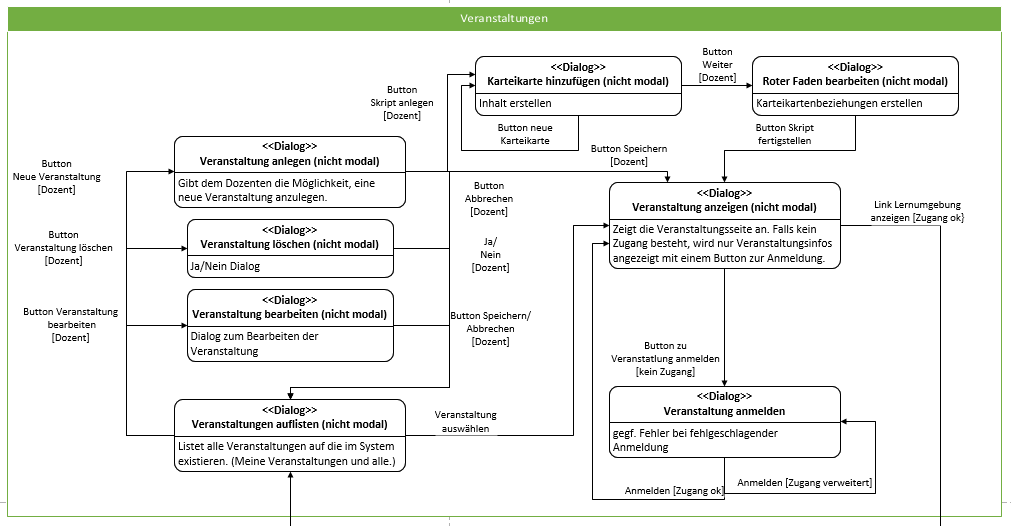
\includegraphics[width=25cm]{Bilder/Mockups/DSDVeranstaltungen.png}
	\caption{Veranstaltungsübersicht und -verwaltung für Dozenten und Studenten}
	\label{DSDVeranstaltung}
\end{figure}

\begin{figure}[H]
	\centering
	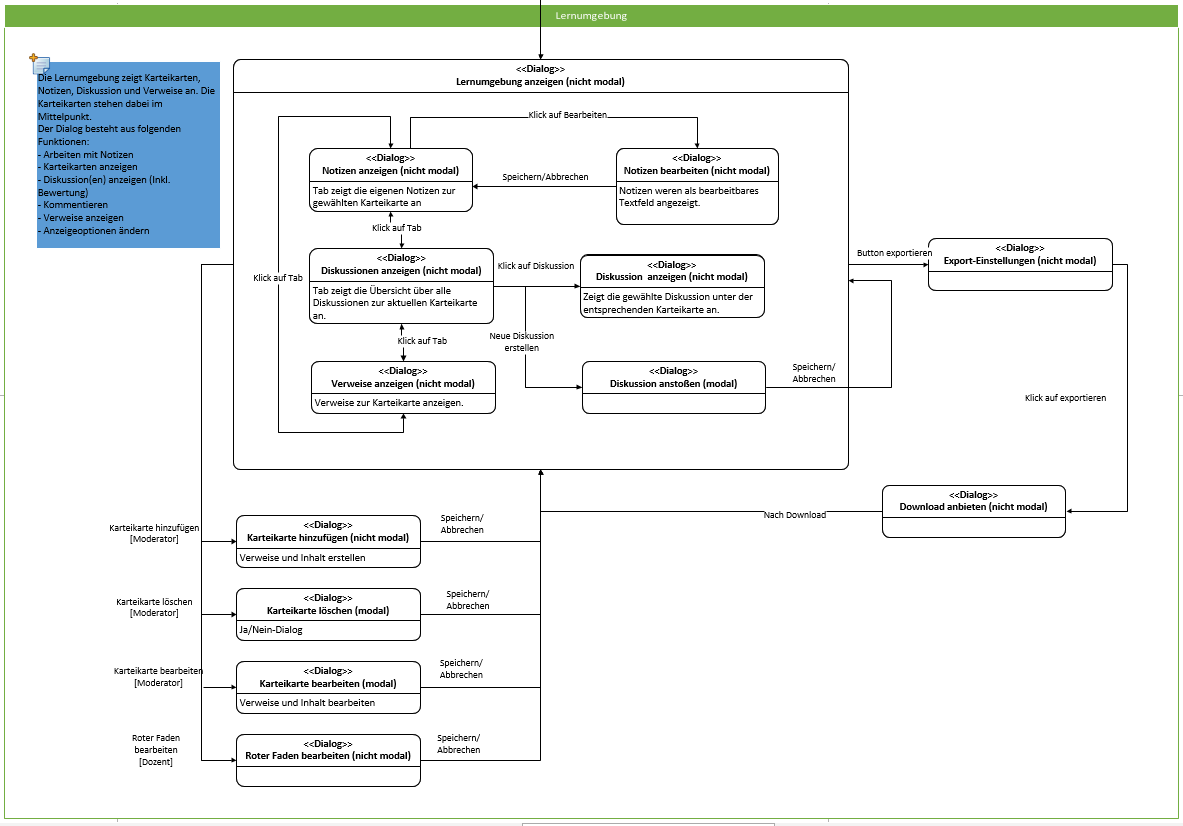
\includegraphics[width=24cm]{Bilder/Mockups/DSDLernumgebung.png}
	\caption{Dialoge für die Lernumgebung. Hierzu gehören Diskussionen, Notizen, Karteikarten, usw...}
	\label{DSDLernumgebung}
\end{figure}

\end{landscape}

\paragraph{Dialoggestaltung} \mbox{}\\
Im folgenden sind die einzelnen Vorschläge für die Dialoggestaltung dargestellt. Diese sind jeweils im Aufbau und Strukturierung gleich. Die darauf ausführbaren Interaktionen werden danach noch einmal im einzelnen beschrieben.\\

\begin{figure}[H]
	\centering
	\paragraph{Startseite}
	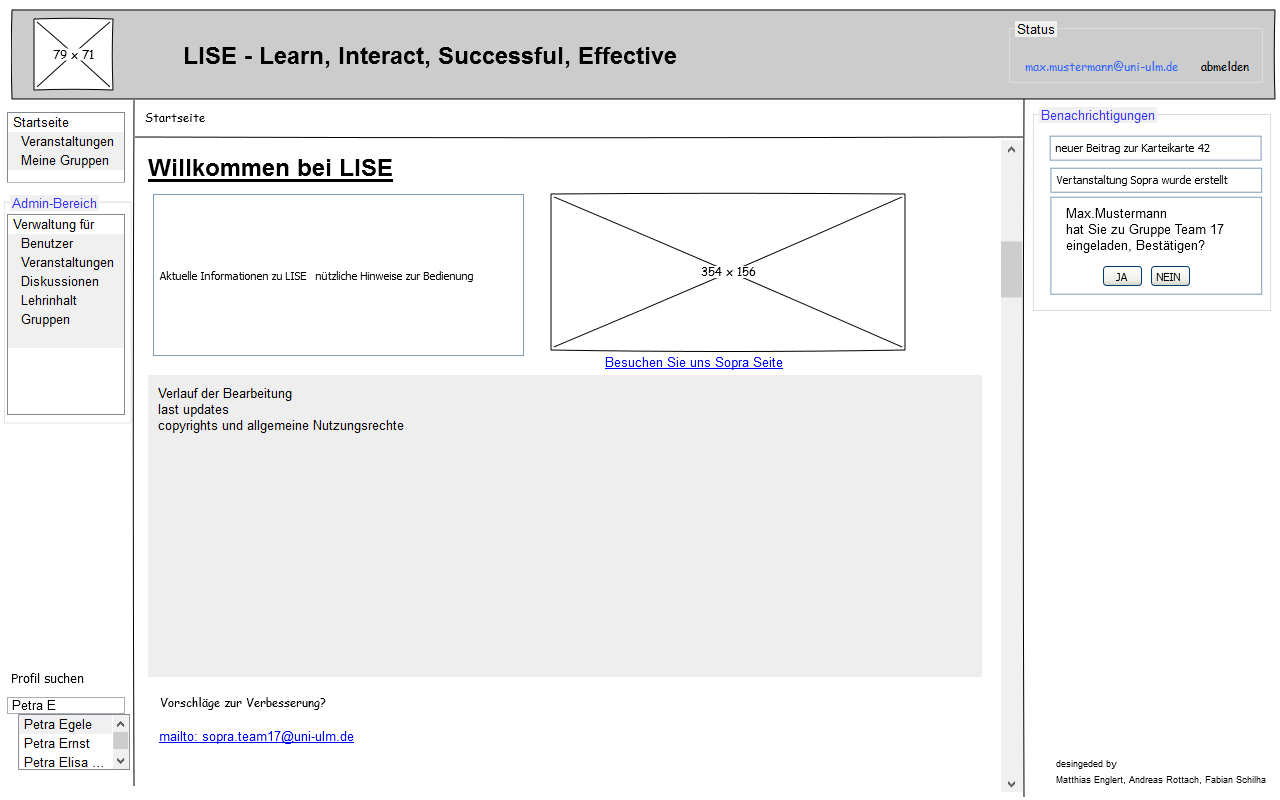
\includegraphics[width=\textwidth]{Bilder/Mockups/GUI/Startseite.png}
	\caption{Startseite}
	\label{GuiStartseite}
\end{figure}

\begin{tabular}{l p{12cm}}
Dialog 	 & \textbf{Startseite} \\ 
Modus & nicht modal\\ 
Beschreibung   	 & Auf dieser Seite werden aktuelle Informationen zum System angezeigt.\\\\

\underline{Interaktion} 	 & Veranstaltungen auflisten\\ 
Beschreibung   	 & Das System wechselt in eine Übersicht, in der die einzelnen Veranstaltungen aufgelistet sind.\\
Vorbedingung	& keine \\
Nachbedingung	& keine \\
Öffnet			& \glqq Veranstaltungen auflisten\grqq \\
Systemoperation & leseVeranstaltungen\\
\end{tabular}\\\\

\begin{tabular}{l p{12cm}}
\underline{Interaktion} 	 & Gruppenübersicht anzeigen\\ 
Beschreibung   	 & Das System wechselt zu einem Dialog, auf dem der Benutzer seine Gruppen verwalten kann.\\
Vorbedingung	& keine \\
Nachbedingung	& keine \\
Öffnet			& \glqq Gruppenübersicht\grqq \\\\
Systemoperation & leseGruppen\\
\end{tabular}\\\\

\begin{tabular}{l p{12cm}}
\underline{Interaktion} 	 & Profil anzeigen\\ 
Beschreibung   	 & Das System wechselt zum persönlichen Profil des Benutzers.\\
Vorbedingung	& keine \\
Nachbedingung	& keine \\
Öffnet			& \glqq Profil anzeigen\grqq \\\\
Systemoperation & leseBenutzerdaten\\
\end{tabular}\\\\

\begin{tabular}{l p{12cm}}
Dialog 	 & \textbf{Profil suchen} \\ 
Modus & nicht modal\\ 
Beschreibung   	 & Der Benutzer kann in dem Textfeld nach anderen Benutzern suchen.\\\\

\underline{Interaktion} 	 & Benutzerprofil auswählen\\ 
Beschreibung   	 & Der Benutzer gibt einen Namen ein und wählt ein vom System vorgeschlagenes Profil aus.\\
Vorbedingung	& keine \\
Nachbedingung	& keine \\
Öffnet			& \glqq Profil anzeigen\grqq \\\\
Systemoperation & sucheBenutzer\\
\end{tabular}\\\\


\begin{figure}[H]
	\centering
	\paragraph{Registrieren}
	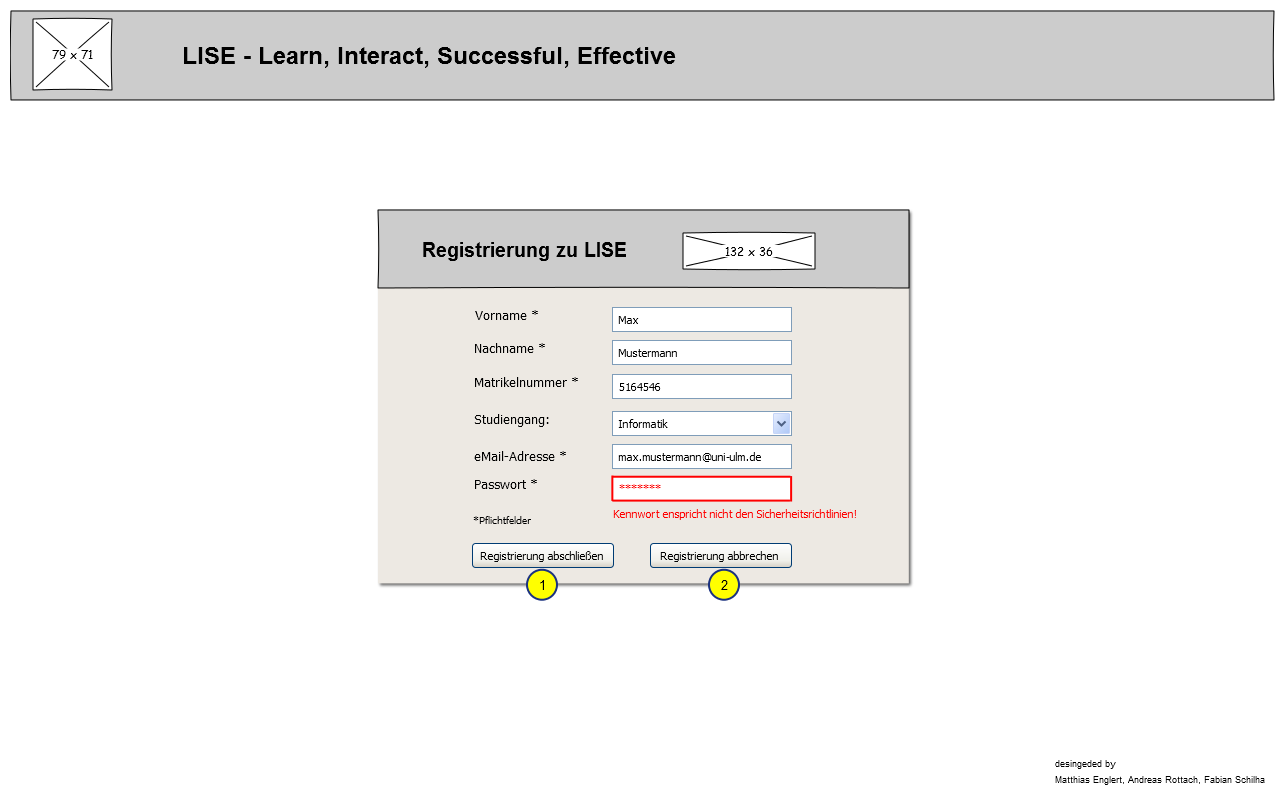
\includegraphics[width=\textwidth]{Bilder/Mockups/GUI/Registrierung.png}
	\caption{Registrieren}
	\label{GuiRegistrieren}
\end{figure}
\begin{tabular}{l p{12cm}}
	Dialog 	 & \textbf{Registrieren} \\ 
	Modus & nicht modal\\ 
	Beschreibung   	 & Der Benutzer kann sich auf dieser Seite registrieren, falls er noch keinen Account im System besitzt. \\\\
	
	\underline{Interaktion} 	 & Registrieren\\ 
	Beschreibung   	 & Siehe oben. Der Benutzer registriert sich im System.\\
	Vorbedingung	& Benutzer ist noch nicht registriert.\\
	Nachbedingung	& Benutzer ist im System registriert. \\
	Öffnet			& Anmelde-Dialog wird geöffnet.\\
	Systemoperation & registrieren\\\\
	
\end{tabular}\\\\

\begin{figure}[H]
	\centering
	\paragraph{Anmelden}
	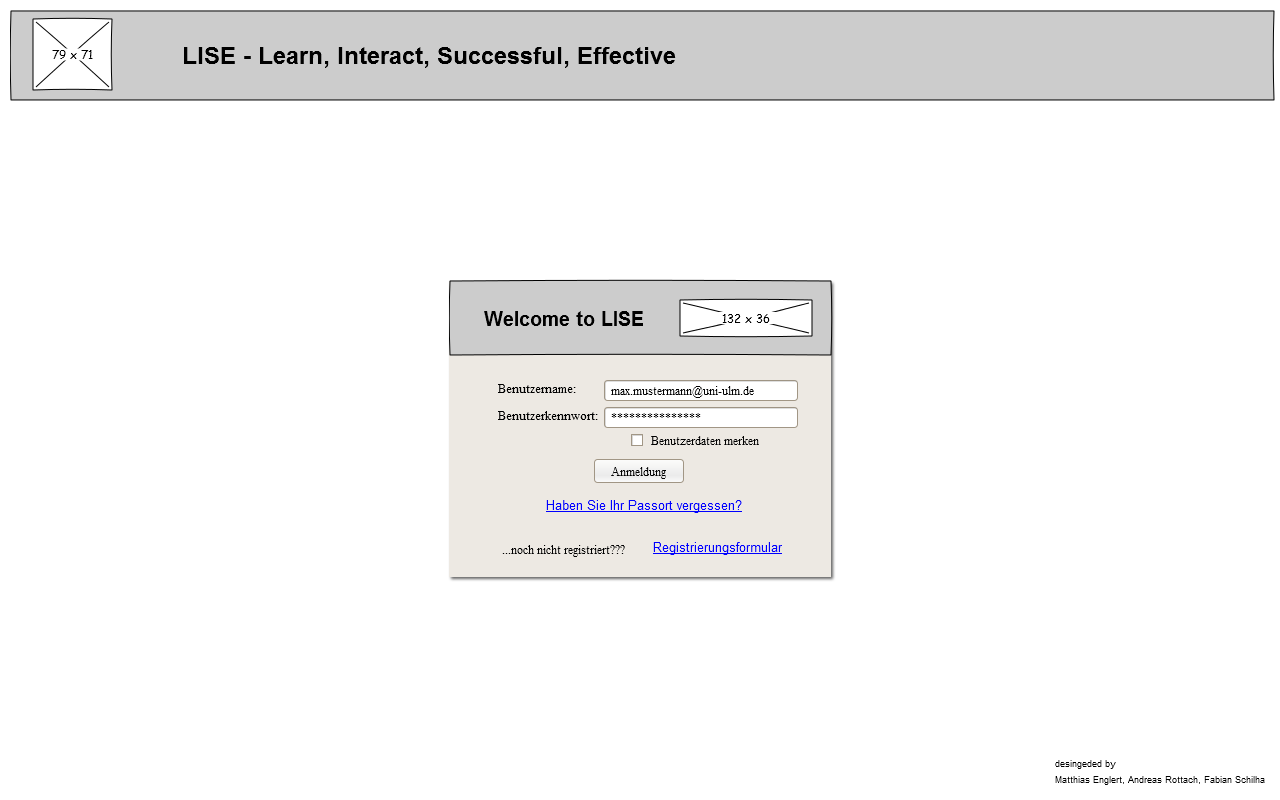
\includegraphics[width=\textwidth]{Bilder/Mockups/GUI/Anmeldung.png}
	\caption{Anmelden}
	\label{GuiAnmelden}
\end{figure}
\begin{tabular}{l p{12cm}}
	Dialog 	 & \textbf{Anmelden} \\ 
	Modus & nicht modal\\ 
	Beschreibung   	& Wenn der Benutzer die Webseite aufruft, landet er auf dem Anmelde-Dialog. \\\\
	
	\underline{Interaktion} 	 & Anmelden\\ 
	Beschreibung   	& Der Benutzer gibt seine Anmeldedaten ein und kann sich in das System einloggen.\\
	Vorbedingung	& Benutzer ist im System registriert.\\
	Nachbedingung	& Das System eröffnet eine Session für den Benutzer. \\
	Öffnet			& Startseite wird geöffnet.\\
	Systemoperation & anmelden,passwortPrüfen\\\\
\end{tabular}

\begin{tabular}{l p{12cm}}
	\underline{Interaktion} 	 & Passwort vergessen\\ 
	Beschreibung   	& Der Benutzer hat sein Passwort vergessen und benötigt Hilfe.\\
	Vorbedingung	& Benutzer ist im System registriert und weiß sein Passwort nicht mehr.\\
	Nachbedingung	& keine \\
	Öffnet			& Dialog \glqq Passwort zurücksetzen\grqq\\\\
\end{tabular}

\begin{tabular}{l p{12cm}}
	\underline{Interaktion} 	 & Registrierung starten\\ 
	Beschreibung   	& Der Benutzer hat keinen Account und möchte sich im System registrieren.\\
	Vorbedingung	& keine\\
	Nachbedingung	& keine \\
	Öffnet			& Dialog \glqq Registrieren\grqq\\\\
\end{tabular}\\\\

\begin{figure}[H]
	\centering
	\paragraph{Passwort zurücksetzen}
	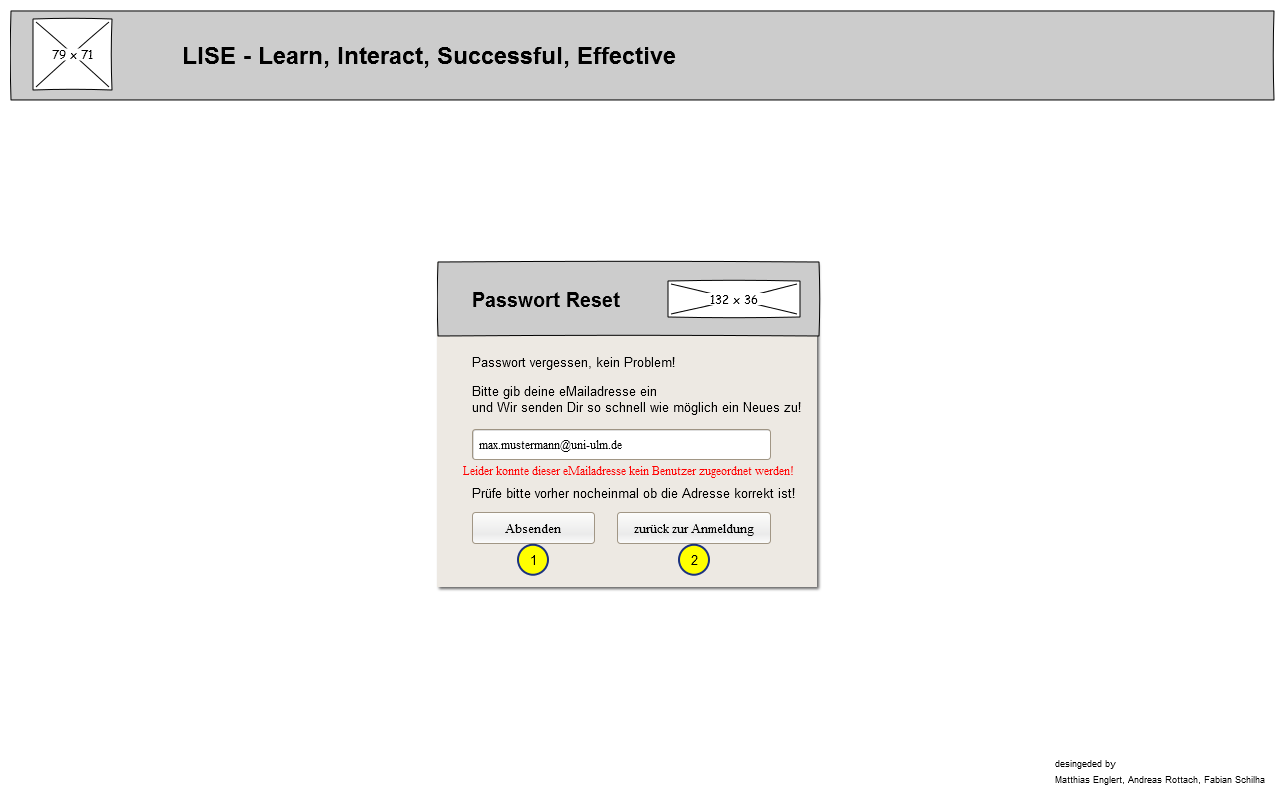
\includegraphics[width=\textwidth]{Bilder/Mockups/GUI/PasswortVergessen.png}
	\caption{Passwort zurücksetzen}
	\label{GuiPasswortVergessen}
\end{figure}
\begin{tabular}{l p{12cm}}
	Dialog 	 & \textbf{Passwort zurücksetzen} \\ 
	Modus & nicht modal\\ 
	Beschreibung   	& Wenn der Benutzer sein Passwort vergessen hat, muss er seine Mail-Adresse angeben und erhält eine Mail mit einem default-Passwort. \\\\
	
	\underline{Interaktion} 	 & Passwort zurücksetzen\\ 
	Beschreibung   	& Der Benutzer setzt sein Passwort zurück durch Klicken auf Button 1.\\
	Vorbedingung	& Benutzer ist im System registriert.\\
	Nachbedingung	& Passwort ist zurückgesetzt. Der Nutzer erhält eine eMail mit dem neuen Passwort. \\
	Öffnet			& Dialog \glqq Anmelden\grqq.\\
	Systemoperation & resetPasswort\\\\
\end{tabular}

\begin{figure}[H]
	\centering
	\paragraph{Profil anzeigen}
	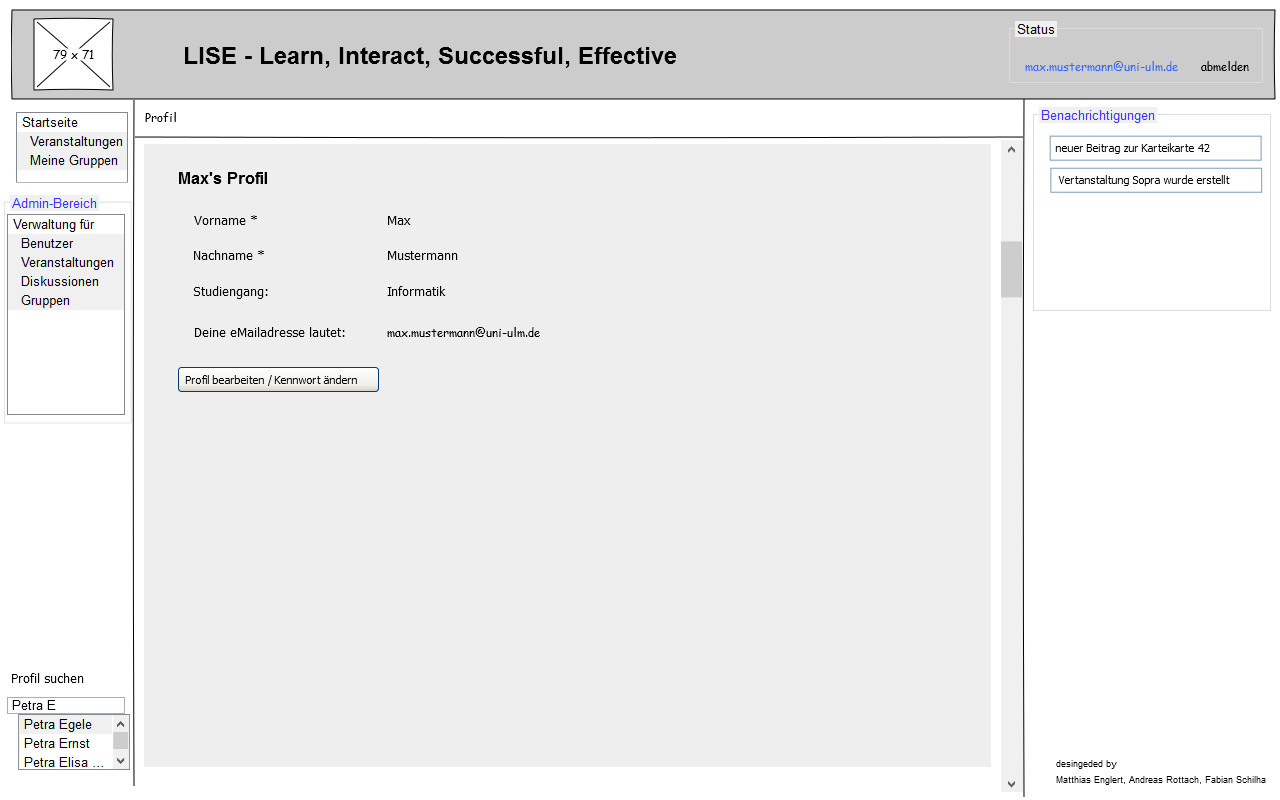
\includegraphics[width=\textwidth]{Bilder/Mockups/GUI/ProfilAnzeigen.png}
	\caption{Profil anzeigen}
	\label{ProfilAnzeigen}
\end{figure}
\begin{tabular}{l p{12cm}}
Dialog 	 & \textbf{Profil anzeigen} \\ 
Modus & nicht modal\\ 
Beschreibung   	 & Der Dialog zeigt die persönlichen Daten eines Benutzers an.\\\\

\underline{Interaktion} 	 & Profil bearbeiten / Kennwort ändern\\ 
Beschreibung   	 & Mit dieser Interaktion kann das Profil bearbeitet werden.\\
Vorbedingung	& Es handelt sich um das eigene Profil \\
Nachbedingung	& keine \\
Öffnet			& \glqq Profil bearbeiten\grqq \\\\
\end{tabular}\\\\

\begin{figure}[H]
	\centering
	\paragraph{Profil bearbeiten}
	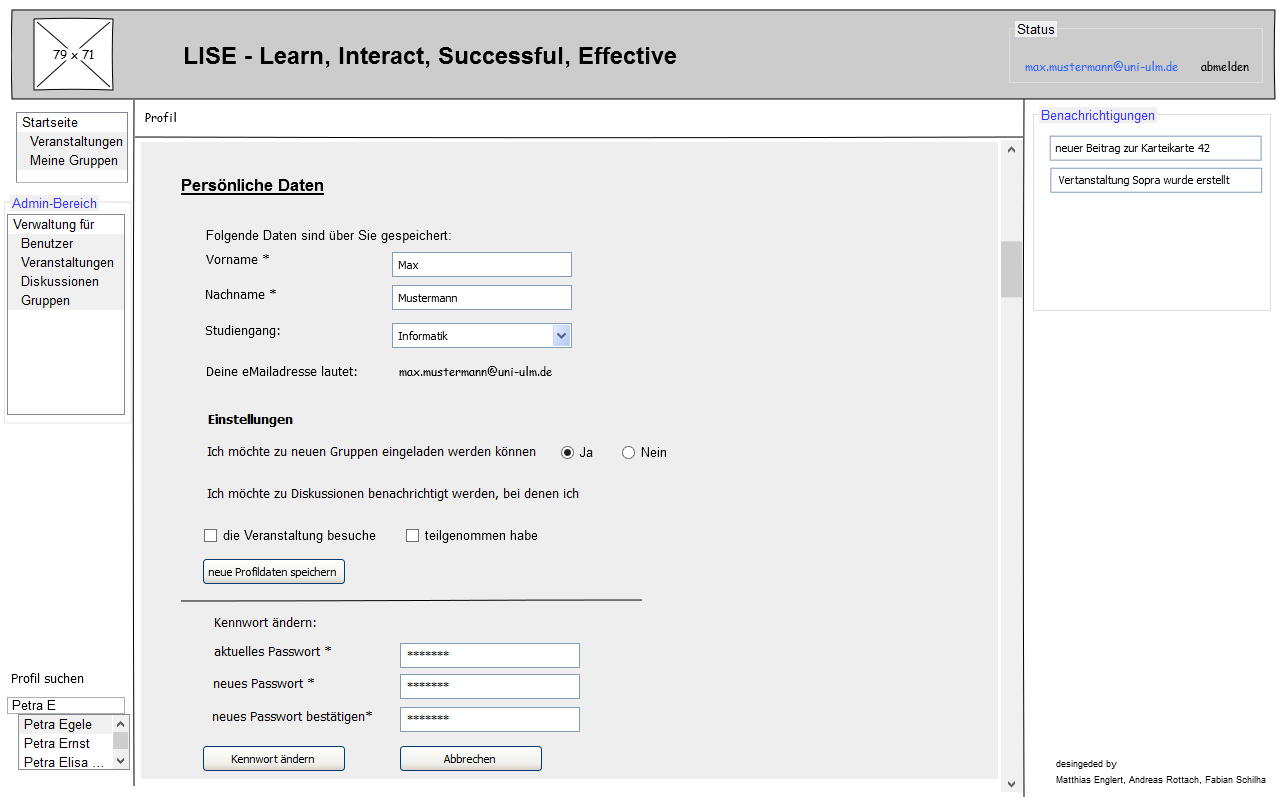
\includegraphics[width=\textwidth]{Bilder/Mockups/GUI/ProfilBearbeiten.png}
	\caption{Profil bearbeiten}
	\label{ProfilBearbeiten}
\end{figure}

\begin{tabular}{l p{12cm}}
Dialog 	 & \textbf{Profil bearbeiten} \\ 
Modus & nicht modal\\ 
Beschreibung   	 & Der Dialog zeigt die persönlichen Daten des Benutzers und Einstellungen zu Gruppen und Diskussionen an. Manche Daten wie z.B Vor- und Nachname sind editierbar. Das Feld Email-Adresse ist nicht editierbar, da es zur Identifikation des Benutzers dient.\\\\

\underline{Interaktion}  	 & neue Profildaten speichern\\ 
Beschreibung   	 & Der Benutzer gibt in die Textfelder seine Änderungen ein, die dann vom System gespeichert werden. Bei Fehleingaben werden die entsprechenden Textfelder markiert.\\
Vorbedingung   	 & Alle Felder sind ausgefüllt\\
Nachbedingung 	 & Profildaten sind gespeichert\\
Öffnet			 & \glqq Profil anzeigen\grqq\\
Systemoperation & ändereBenutzerdaten\\\\
\end{tabular}\\\\

\begin{tabular}{l p{12cm}}
\underline{Interaktion}  	 & Kennwort ändern\\ 
Beschreibung   	 & Der Benutzer gibt sein aktuelles und sein neues Passwort ein. Das neue Passwort wird gespeichert. Macht der Benutzer einen Fehler, bleibt er auf dem aktuellen Dialog und es werden die entsprechenden Textfelder rot markiert. \\
Vorbedingung   	 & Aktuelles Passwort ist korrekt. Neues Passwort ist lang genug. Die Textfelder neues Passwort und neues Passwort bestätigen stimmen überein\\
Nachbedingung 	 & neues Kennwort wird gespeichert\\
Öffnet			 & \glqq Profil anzeigen\grqq\\
Systemoperation & passwortPrüfen\\\\
\end{tabular}\\\\

\begin{tabular}{l p{12cm}}
\underline{Interaktion} 	 & Abbrechen\\ 
Beschreibung   	 & Die Bearbeitung des Profils wird abgebrochen. \\
Vorbedingung   	 & keine\\
Nachbedingung 	 & Die Änderungen des Benutzers werden nicht gespeichert\\
Öffnet			 & \glqq Profil anzeigen\grqq\\\\
\end{tabular}\\\\  

\begin{figure}[H]
	\centering
	\paragraph{Veranstaltungen auflisten}
	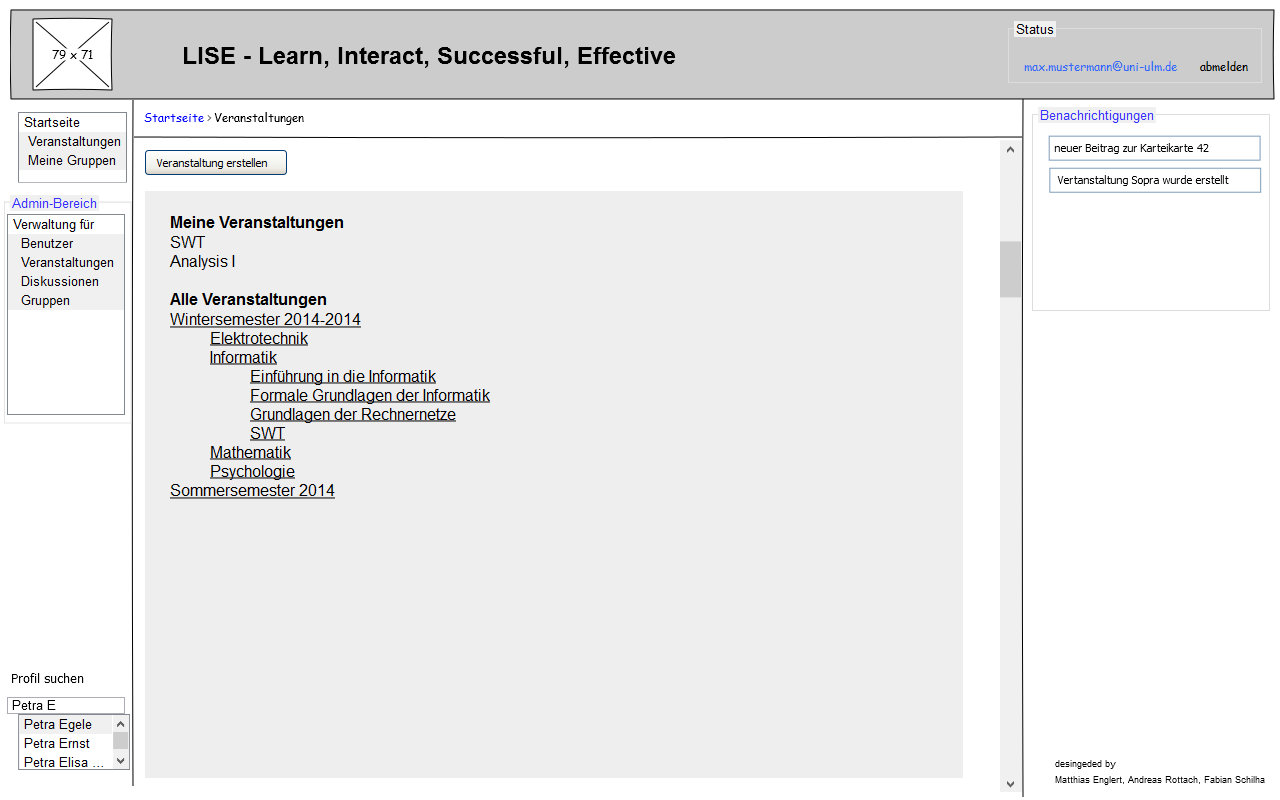
\includegraphics[width=\textwidth]{Bilder/Mockups/GUI/VeranstaltungenAuflisten.png}
	\caption{Veranstaltungen auflisten}
	\label{VeranstaltungenAuflisten}
\end{figure}

\begin{tabular}{l p{12cm}}
Dialog 	 & \textbf{Veranstaltungen auflisten} \\ 
Modus & nicht modal\\ 
Beschreibung   	 & Auf dieser Oberfläche werden alle Veranstaltungen geordnet nach Semester und Studienfach aufgelistet. Ein Dozent hat zusätzlich noch die Möglichkeit neue Veranstaltungen zu erstellen\\\\

\underline{Interaktion} 	 & Auswahl des Semesters\\ 
Beschreibung   	 & Der Benutzer wählt beispielsweise den Punkt Wintersemester 2014/2015. Dann werden alle Studiengänge in diesem Semester als Unterpunkte angezeigt\\
Vorbedingung	& keine \\
Nachbedingung	& keine \\
Öffnet			& kein neuer Dialog wird geöffnet\\
\end{tabular}\\\\ 

\begin{tabular}{l p{12cm}}
\underline{Interaktion} 	 & Auswahl eines Studiengangs\\ 
Beschreibung   	 & Nachdem der Benutzer das Semester gewählt hat, kann er einen Studiengang anklicken. Dann werden alle Veranstaltungen dieses Studiengangs als Unterpunkte angezeigt\\
Vorbedingung	& keine \\
Nachbedingung	& keine \\
Öffnet			& kein neuer Dialog wird geöffnet\\
\end{tabular}\\\\ 

\begin{tabular}{l p{12cm}}
\underline{Interaktion} 	 & Auswahl einer Veranstaltung\\ 
Beschreibung   	 & Nachdem der Benutzer den Studiengang gewählt hat, kann er sich eine Veranstaltung aussuchen.\\
Vorbedingung	& keine \\
Nachbedingung	& keine \\
Öffnet			& \glqq Veranstaltung\grqq, wenn der Benutzer für die Veranstaltung eingetragen ist. Falls nicht wird der Dialog \glqq Veranstaltung eintragen\grqq geöffnet \\
\end{tabular}\\\\
		
\begin{tabular}{l p{12cm}}	
\underline{Interaktion} 	 & Veranstaltung erstellen\\ 
Beschreibung   	 & Ein Dozent kann für seine Vorlesung eine neue Veranstaltung anlegen.\\
Vorbedingung	& als Dozent angemeldet \\
Nachbedingung	& keine \\
Öffnet 			& \glqq Veranstaltung anlegen\grqq \\\\
\end{tabular}\\\\

\begin{figure}[H]
	\centering
	\paragraph{Veranstaltung anlegen}
	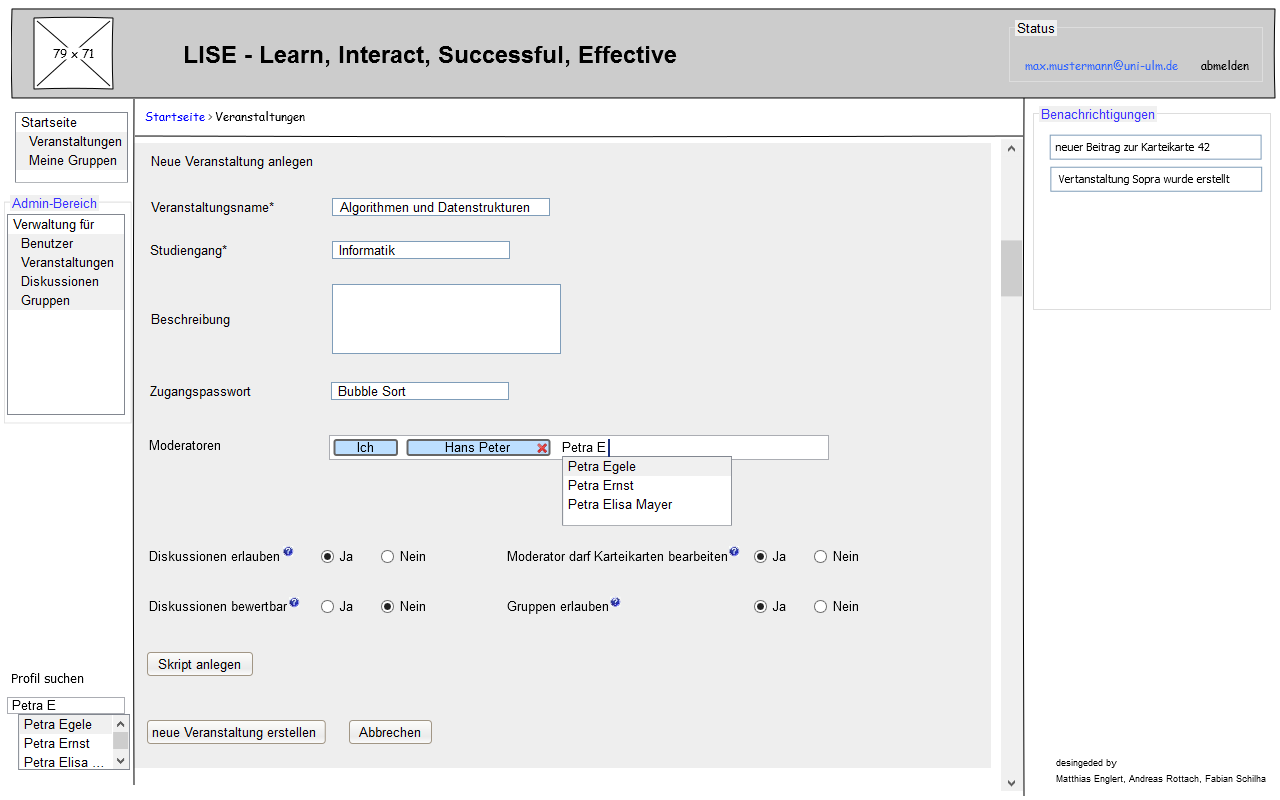
\includegraphics[width=\textwidth]{Bilder/Mockups/GUI/VeranstaltungAnlegen.png}
	\caption{Veranstaltung anlegen}
	\label{VeranstaltungAnlegen}
\end{figure}

\begin{tabular}{l p{12cm}}
Dialog 	 & \textbf{Veranstaltung anlegen} \\ 
Modus & nicht modal\\ 
Beschreibung   	 & Mit diesem Dialog kann ein Dozent eine neue Veranstaltung anlegen. Der Dialog besteht aus Textfeldern, mit denen der Dozent die Daten der Veranstaltung eingibt. Der Inhalt des Textfelds \glqq Beschreibung\grqq steht später dann auf der Anfangsseite der Veranstaltung, damit ein Benutzer weiß, um was es in der Veranstaltung geht. Der Dozent kann mehrere Moderatoren festlegen. Er selbst ist immer auch ein Moderator. Der Dozent kann einstellen, ob es zu seiner Veranstaltung Diskussionen geben soll und ob man die Qualität der Diskussionen bewerten darf. Außerdem kann er festlegen, ob die Moderatoren nur für die Verwaltung von Diskussionen zuständig sind oder ob sie auch Karteikarten bearbeiten dürfen. Wenn der Dozent nicht möchte, dass Diskussionen nur in einzelnen Gruppen stattfinden, dann kann er die Gruppenbildung für seine Veranstaltung verbieten. \\\\

\underline{Interaktion}  	 & Skript anlegen\\ 
Beschreibung   	 & Mit dieser Option kann der Dozent ein initiales Skript erstellen.\\
Vorbedingung   	 & keine\\
Nachbedingung 	 & Die Veranstaltungsdaten, die der Dozent schon eingegeben hat, bleiben erhalten nachdem er das initiale Skript erstellt hat.\\
Öffnet			 & \glqq Karteikarte erstellen\grqq \\
\end{tabular}\\\\

\begin{tabular}{l p{12cm}}
\underline{Interaktion}  	 & neue Veranstaltung erstellen\\ 
Beschreibung   	 & Der Dozent bestätigt die Daten, die er für die Veranstaltung eingetragen hat und eine neue Veranstaltung wird erstellt. Wurden falsche Eingaben gemacht werden die entsprechenden Textfelder rot markiert. \\
Vorbedingung   	 & Alle Pflichtfelder sind ausgefüllt.\\
Nachbedingung	 & keine\\
Öffnet			 & \glqq Veranstaltung \grqq, in dem die gerade erstellte Veranstaltung angezeigt wird. \\
Systemoperation & veranstaltungAnlegen\\\\
\end{tabular}\\\\

\begin{tabular}{l p{12cm}}
\underline{Interaktion}  	 & Abbrechen\\ 
Beschreibung   	 & Es wird keine neue Veranstaltung erstellt und die eingegebenen Daten verworfen.  \\
Vorbedingung	 & keine \\
Nachbedingung	 & keine \\
Öffnet			 & \glqq Veranstaltungen auflisten\grqq \\\\
\end{tabular}\\\\

\begin{figure}[H]
	\centering
	\paragraph{Veranstaltung bearbeiten}
	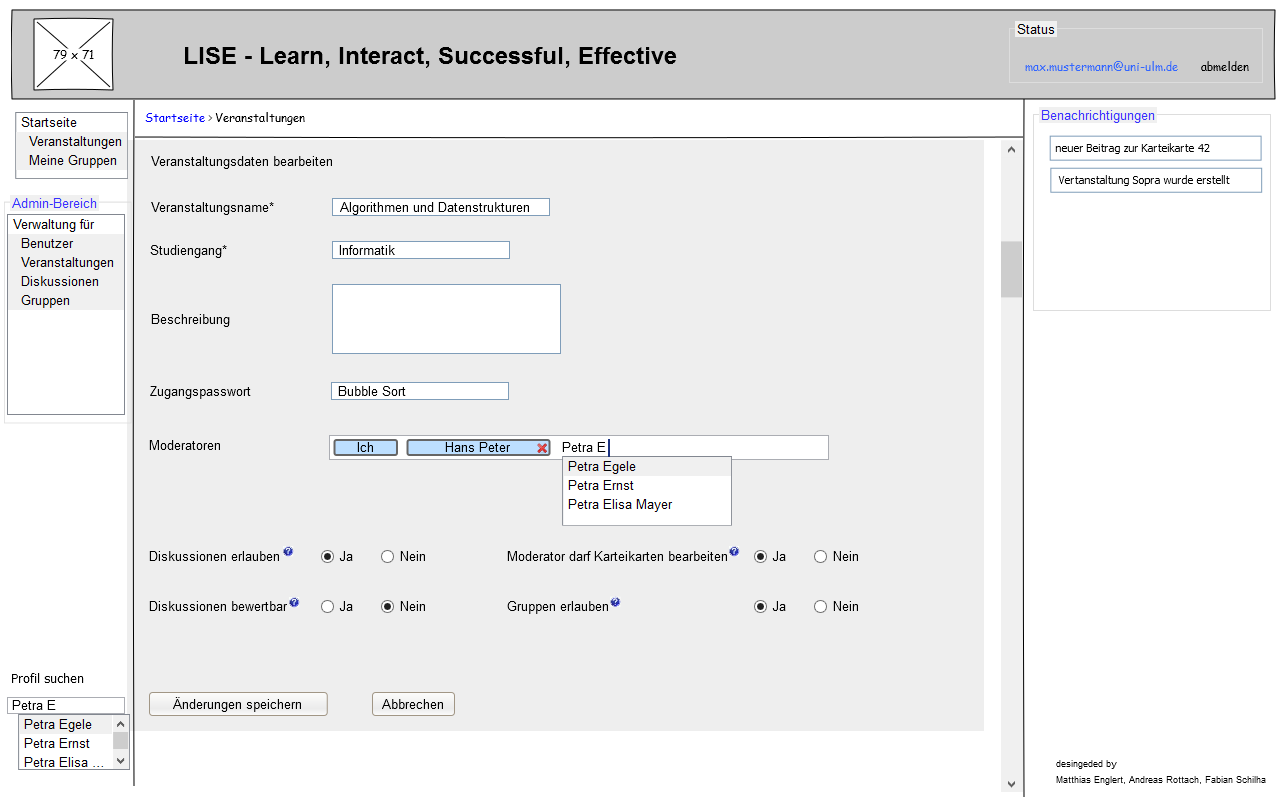
\includegraphics[width=\textwidth]{Bilder/Mockups/GUI/VeranstaltungBearbeiten.png}
	\caption{Veranstaltung bearbeiten}
	\label{VeranstaltungBearbeiten}
\end{figure}

\begin{tabular}{l p{12cm}}
Dialog 	 & \textbf{Veranstaltung bearbeiten} \\ 
Modus & nicht modal\\ 
Beschreibung   	 & Hier kann ein Dozent die Daten seiner Veranstaltung bearbeiten. \\\\

\underline{Interaktion}  	 & Änderungen speichern\\ 
Beschreibung   	 & Der Dozent bestätigt seine Änderungen. Wurden falsche Eingaben gemacht werden die entsprechenden Textfelder rot markiert. \\
Vorbedingung   	 & Alle Pflichtfelder sind ausgefüllt.\\
Nachbedingung	 & keine\\
Öffnet			 & \glqq Veranstaltung \grqq, in dem die gerade bearbeitete Veranstaltung angezeigt wird. \\
Systemoperation & veranstaltungBearbeiten\\\\
\end{tabular}\\\\

\begin{tabular}{l p{12cm}}
\underline{Interaktion}  	 & Abbrechen\\ 
Beschreibung   	 & Es werden keine Änderungen an der Veranstaltung vorgenommen.  \\
Vorbedingung	 & keine \\
Nachbedingung	 & keine \\
Öffnet			 & \glqq Veranstaltung\grqq \\\\
\end{tabular}\\\\

\begin{figure}[H]
	\centering
	\paragraph{Veranstaltung eintragen}
	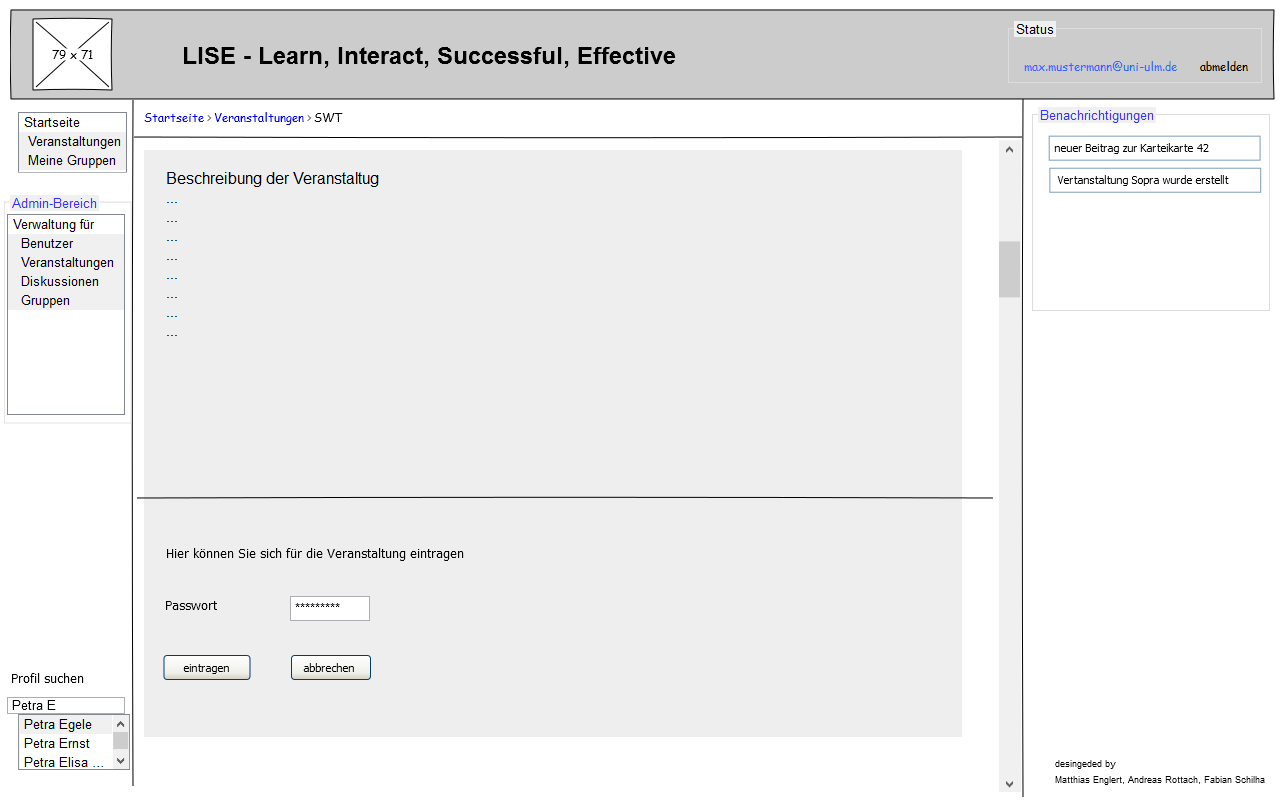
\includegraphics[width=\textwidth]{Bilder/Mockups/GUI/VeranstaltungEintragen.png}
	\caption{Veranstaltung eintragen}
	\label{VeranstaltungEintragen}
\end{figure}

\begin{tabular}{l p{12cm}}
Dialog 	 & \textbf{Veranstaltung eintragen} \\ 
Modus & nicht modal\\ 
Beschreibung   	 & Wenn der Benutzer noch nicht für diese Veranstaltung eingetragen ist, bekommt er nur eine Beschreibung dieser Veranstaltung und die Möglichkeit sich einzutragen. Dabei kann ein Passwort notwendig sein, das der verantwortliche Dozent beim Erstellen der Veranstaltung festlegen kann.\\\\ 

\underline{Interaktion}  	 & eintragen\\ 
Beschreibung   	 & Der Benutzer gibt evtl. ein Passwort ein und bestätigt, dass er sich für diese Veranstaltung eintragen möchte.  \\
Vorbedingung	 & Passwort korrekt \\
Nachbedingung	 & Der Benutzer ist nun dauerhaft für diese Veranstaltung eingetragen \\
Öffnet			 & \glqq Veranstaltungen auflisten\grqq \\
Systemoperation & veranstaltungEintragen,pruefePasswortVeranstaltung\\\\
\end{tabular}\\\\

\begin{tabular}{l p{12cm}}
\underline{Interaktion}  	 & Abbrechen\\ 
Beschreibung   	 & Der Benutzer wird nicht eingetragen.  \\
Vorbedingung	 & keine \\
Nachbedingung	 & keine \\
Öffnet			 & \glqq Veranstaltungen auflisten\grqq \\\\

\end{tabular}\\\\

\begin{figure}[H]
	\centering
	\paragraph{Veranstaltung}
	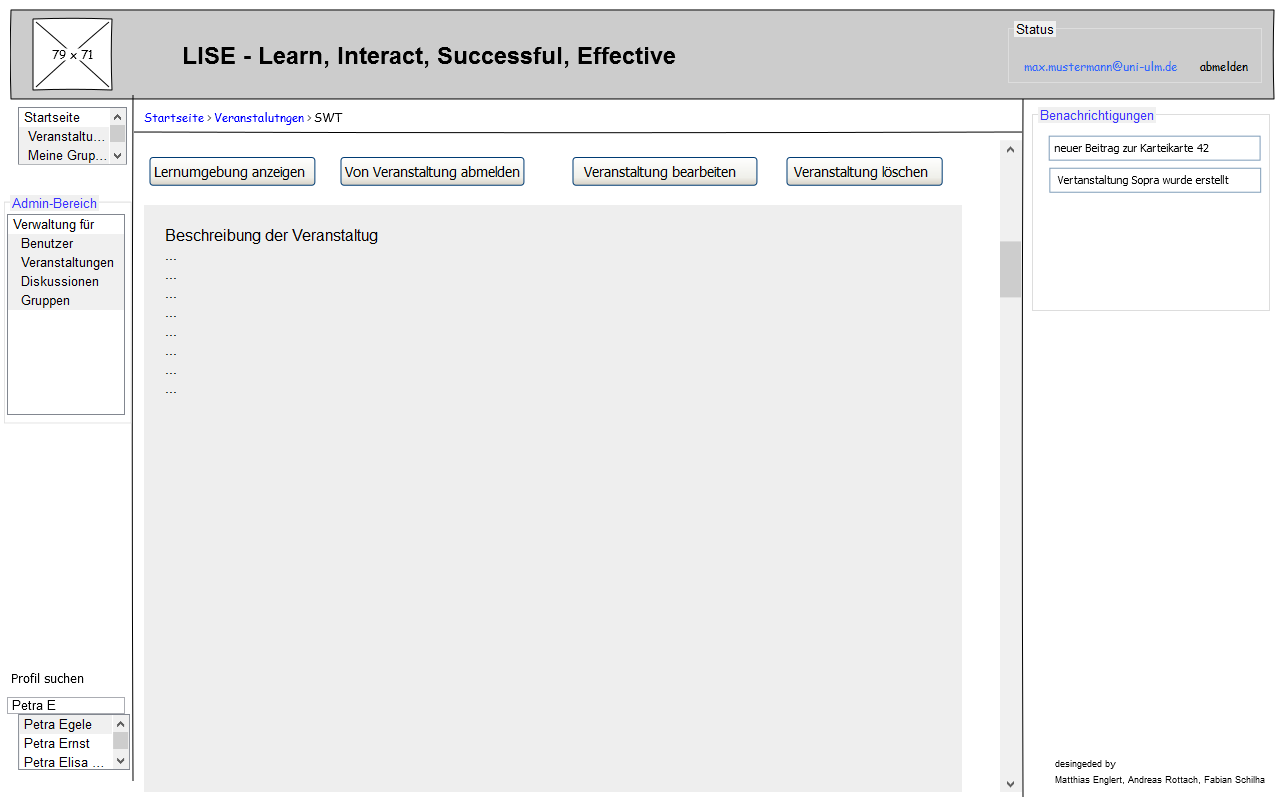
\includegraphics[width=\textwidth]{Bilder/Mockups/GUI/Veranstaltung.png}
	\caption{Veranstaltung}
	\label{Veranstaltung}
\end{figure}

\begin{tabular}{l p{12cm}}
Dialog 	 & \textbf{Veranstaltung} \\ 
Modus & nicht modal\\ 
Beschreibung   	 & Auf diesem Dialog wird eine konkrete Veranstaltung angezeigt. Es wird eine kurze Beschreibung gegeben, um dem Benutzer allgemeine Informationen zu dieser Veranstaltung bereit zu stellen. Da das System eine E-Learning Plattform ist, gibt es zu jeder Veranstaltung eine Lernumgebung.\\\\ 

\underline{Interaktion}  	 & Lernumgebung anzeigen\\ 
Beschreibung   	 & Der Benutzer möchte zur Lernumgebung wechseln.  \\
Vorbedingung	 & keine \\
Nachbedingung	 & keine \\
Öffnet			 & \glqq Lernumgebung anzeigen\grqq und \glqq Notizen einsehen\grqq \\
Systemoperation & karteikartenLesen\\\\
\end{tabular}\\\\

\begin{tabular}{l p{12cm}}
\underline{Interaktion}  	 & Von Veranstaltung abmelden\\ 
Beschreibung   	 & Der Benutzer wird aus der Veranstaltung gelöscht.  \\
Vorbedingung	 & keine \\
Nachbedingung	 & Der Benutzer hat nun keinen Zugriff und bekommt keine Benachrichtigungen mehr zu dieser Veranstaltung. \\
Öffnet			 & \glqq Veranstaltungen auflisten\grqq \\
Systemoperation & vonVeranstaltungAbmelden\\\\
\end{tabular}\\\\

\begin{tabular}{l p{12cm}}
\underline{Interaktion}  	 & Veranstaltung bearbeiten\\ 
Beschreibung   	 & Der Dozent dieser Veranstaltung möchte bestimmte Daten der Veranstaltung ändern.  \\
Vorbedingung	 & als Dozent angemeldet, der die Veranstaltung erstellt hat \\
Nachbedingung	 & keine \\
Öffnet			 & \glqq Veranstaltung bearbeiten\grqq \\
Systemoperation & leseVeranstaltung\\\\
\end{tabular}\\\\

\begin{tabular}{l p{12cm}}
\underline{Interaktion}  	 & Veranstaltung löschen\\ 
Beschreibung   	 & Der Dozent möchte seine Veranstaltung löschen.  \\
Vorbedingung	 & als Dozent angemeldet, der die Veranstaltung erstellt hat \\
Nachbedingung	 & keine \\
Öffnet			 & \glqq Ja/Nein Dialog\grqq \\
Systemoperation & veranstaltungLöschen\\\\
\end{tabular}\\\\

\begin{figure}[H]
	\centering
	\paragraph{Gruppe erstellen}
	\includegraphics[width=\textwidth]{Bilder/Mockups/GUI/GruppeErstellen.png}
	\caption{Gruppe erstellen}
	\label{GuiGruppeErstellen}
\end{figure}
\begin{tabular}{l p{12cm}}
	Dialog 	 & \textbf{Gruppe erstellen} \\ 
	Modus & nicht modal\\ 
	Beschreibung   	& Dieser Dialog wird verwendet um eine neue Gruppe anzulegen. Der Nutzer muss einen, innerhalb der Veranstaltung eindeutigen Namen wählen, die Veranstaltung selbst wählen und eine Beschreibung eingeben. Nun kann er Mitglieder hinzufügen. \\\\
	
	\underline{Interaktion} 	 & Mitglieder hinzufügen\\ 
	Beschreibung   	& Der Ersteller kann Benutzer hinzufügen, indem er den Namen des Nutzers in das Textfeld schreibt. Während dem Schreiben werden ihm Vorschläge anzeigt. Durch Drücken der Enter-Taste wird der Nutzer als Mitglied hinzugefügt. Über das kleine rote X kann man den Benutzer wieder entfernen.\\
	Vorbedingung	& keine \\
	Nachbedingung	& keine \\
	Öffnet			& keinen\\\\
\end{tabular}

\begin{tabular}{l p{12cm}}
	\underline{Interaktion} 	 & Gruppe anlegen\\ 
	Beschreibung   	& Der Ersteller schließt den Vorgang ab indem er auf Button 2 klickt. Nun ist eine neue Gruppe erstellt.\\
	Vorbedingung	& keine \\
	Nachbedingung	& keine \\
	Öffnet			& Dialog \glqq Gruppenübersicht\grqq.\\
	Systemoperation & gruppeErstellen\\\\
\end{tabular}

\begin{tabular}{l p{12cm}}
	\underline{Interaktion} 	 & Vorgang abbrechen\\ 
	Beschreibung   	& Der Vorgang kann abgebrochen werden, indem man auf Button 3 klickt.\\
	Vorbedingung	& keine \\
	Nachbedingung	& keine \\
	Öffnet			& Dialog \glqq Gruppenübersicht\grqq.\\
	Systemoperation & gruppenLesen\\\\
\end{tabular}

\begin{figure}[H]
	\centering
	\paragraph{Gruppenübersicht}
	\includegraphics[width=\textwidth]{Bilder/Mockups/GUI/Gruppenuebersicht.png}
	\caption{Gruppenübersicht}
	\label{GuiGruppenuebersicht}
\end{figure}
\begin{tabular}{l p{12cm}}
	Dialog 	 & \textbf{Gruppenübersicht} \\ 
	Modus & nicht modal\\ 
	Beschreibung   	& Hier bekommt der Benutzer eine Übersicht über alle Gruppen, in denen er Mitglied ist oder die er erstellt hat. Der Administrator hat hier alle Rechte. Er kann alle Gruppen löschen, alle bearbeiten und neue anlegen, unabhängig davon, ob er Mitglied in einer Gruppe ist.\\\\
	
	\underline{Interaktion} 	 & Mitgliedschaft beenden\\ 
	Beschreibung   	& Durch Klicken auf ein rotes X öffnet sich ein Bestätigungsdialog und die Mitgliedschaft wird beendet. Ist man selbst Ersteller der Gruppe, so wird die Gruppe ebenfalls entfernt.\\
	Vorbedingung	& keine \\
	Nachbedingung	& keine \\
	Öffnet			& Dialog \glqq Gruppenübersicht\grqq.\\
	Systemoperation & gruppeVerlassen\\\\
\end{tabular}

\begin{tabular}{l p{12cm}}
	\underline{Interaktion} 	 & Gruppe bearbeiten\\ 
	Beschreibung   	& Der Ersteller einer Gruppe kann sie bearbeiten, indem er auf das kleine Zahnrad klickt.\\
	Vorbedingung	& keine \\
	Nachbedingung	& keine \\
	Öffnet			& Dialog \glqq Gruppen bearbeiten\grqq.\\
	Systemoperation & gruppeLesen\\\\
\end{tabular}

\begin{tabular}{l p{12cm}}
	\underline{Interaktion} 	 & Gruppe erstellen\\ 
	Beschreibung   	& Der Benutzer kann eine neue Gruppe erstellen, indem er auf Button 2 klickt.\\
	Vorbedingung	& keine \\
	Nachbedingung	& keine \\
	Öffnet			& Dialog \glqq Gruppen anlegen\grqq.\\\\
\end{tabular}

\begin{figure}[H]
	\centering
	\paragraph{Gruppe bearbeiten}
	\includegraphics[width=\textwidth]{Bilder/Mockups/GUI/GruppeBearbeiten.png}
	\caption{Gruppe bearbeiten}
	\label{GuiGruppeBearbeiten}
\end{figure}
\begin{tabular}{l p{12cm}}
	Dialog 	 & \textbf{Gruppe bearbeiten} \\ 
	Modus & nicht modal\\ 
	Beschreibung   	& Hier kann der Benutzer eine selbst erstellte Gruppe bearbeiten. Das Feld \glqq Veranstaltung\grqq ist nicht mehr editierbar. \\\\
	
	\underline{Interaktion} 	 & Änderungen speichern\\ 
	Beschreibung   	& Durch Klicken auf Button 1 werden die Änderungen übernommen.\\
	Vorbedingung	& keine \\
	Nachbedingung	& keine \\
	Öffnet			& Dialog \glqq Gruppenübersicht\grqq.\\
	Systemoperation & gruppeBearbeiten\\\\
\end{tabular}

\begin{tabular}{l p{12cm}}
	\underline{Interaktion} 	 & Abbrechen\\ 
	Beschreibung   	& Durch Klicken auf Button 2 werden die Änderungen verworfen.\\
	Vorbedingung	& keine \\
	Nachbedingung	& keine \\
	Öffnet			& Dialog \glqq Gruppenübersicht\grqq.\\
	Systemoperation & leseGruppen\\\\
\end{tabular}

\begin{figure}[H]
	\centering
	\paragraph{Benutzerverwaltung}
	\includegraphics[width=\textwidth]{Bilder/Mockups/GUI/Benutzerverwaltung[Admin].png}
	\caption{Benutzerverwaltung}
	\label{GuiBenutzerverwaltung}
\end{figure}
\begin{tabular}{l p{12cm}}
	Dialog 	 & \textbf{Benutzerverwaltung} \\ 
	Modus & nicht modal\\ 
	Beschreibung   	& Der Administrator hat die Möglichkeit den Status von Nutzern zu ändern, indem er den Namen im Textfeld eingibt. Es werden wieder Vorschläge anzeigt und durch das Drücken von Enter wird der Nutzer ausgewählt und die Daten werden unten angezeigt. Hier kann der Administrator den Nutzerstatus ändern oder den Benutzer löschen. \\\\
	
	\underline{Interaktion} 	 & Nutzerstatus ändern\\ 
	Beschreibung   	& Der Administrator kann den Status eines ausgewählten Benutzers ändern, indem er den Typ aus einer Liste wählt. Mögliche Typen wären: Student oder Dozent.\\
	Vorbedingung	& keine \\
	Nachbedingung	& keine \\
	Öffnet			& keinen\\\\
\end{tabular}

\begin{tabular}{l p{12cm}}
	\underline{Interaktion} 	 & Benutzer löschen\\ 
	Beschreibung   	& Durch Klicken auf Button 5 und anschließender Bestätigung kann der Administrator einen Nutzer aus dem System löschen.\\
	Vorbedingung	& keine \\
	Nachbedingung	& keine \\
	Öffnet			& Dialog \glqq Benutzerverwaltung\grqq.\\
	Systemoperation & benutzerLöschen\\\\
\end{tabular}

\begin{tabular}{l p{12cm}}
	\underline{Interaktion} 	 & Abbrechen\\ 
	Beschreibung   	& Durch Klicken auf Button 2 werden die Änderungen verworfen.\\
	Vorbedingung	& keine \\
	Nachbedingung	& keine \\
	Öffnet			& Dialog \glqq Benutzerverwaltung\grqq.\\\\
\end{tabular}

\begin{tabular}{l p{12cm}}
	\underline{Interaktion} 	 & Änderungen speichern\\ 
	Beschreibung   	& Der Administrator kann den Vorgang abbrechen, indem er auf Button 6 klickt.\\
	Vorbedingung	& keine \\
	Nachbedingung	& keine \\
	Öffnet			& Dialog \glqq Benutzerverwaltung\grqq.\\
	Systemoperation & benuterstatusÄndern\\\\
\end{tabular}

\begin{figure}[H]
	\centering
	\paragraph{Bestätigungs-Dialog}
	\includegraphics[width=\textwidth]{Bilder/Mockups/GUI/Bestaetigung.png}
	\caption{Bestätigungs-Dialog}
	\label{GuiBestaetigungsDialog}
\end{figure}
\begin{tabular}{l p{12cm}}
	Dialog 	 & \textbf{Bestätigungs-Dialog} \\ 
	Modus & modal\\ 
	Beschreibung   	& Dieser Dialog zeigt jede Art von Bestätigung im System an. \\\\
	
	\underline{Interaktion} 	 & Bestätigen\\ 
	Beschreibung   	& Schließt den Dialog und bestätigt ihn.\\
	Vorbedingung	& keine \\
	Nachbedingung	& keine \\
	Öffnet			& keinen\\\\
\end{tabular}

\begin{tabular}{l p{12cm}}
	\underline{Interaktion} 	 & Abbrechen\\ 
	Beschreibung   	& Schließt den Dialog und bricht die Aktion ab.\\
	Vorbedingung	& keine \\
	Nachbedingung	& keine \\
	Öffnet			& keinen\\\\
\end{tabular}

\begin{figure}[H]
	\centering
	\paragraph{Fehler-Dialog}
	\includegraphics[width=\textwidth]{Bilder/Mockups/GUI/Fehler.png}
	\caption{Fehler-Dialog}
	\label{GuiFehlerDialog}
\end{figure}
\begin{tabular}{l p{12cm}}
	Dialog 	 & \textbf{Fehler-Dialog} \\ 
	Modus & modal\\ 
	Beschreibung   	& Dieser Dialog zeigt jede Art von Fehler im System an. \\\\
	
	\underline{Interaktion} 	 & Bestätigen\\ 
	Beschreibung   	& Schließt den Dialog.\\
	Vorbedingung	& keine \\
	Nachbedingung	& keine \\
	Öffnet			& keinen\\\\
\end{tabular}


\begin{figure}[H]
	\centering
	\paragraph{Exporteinstellungen}
	\includegraphics[width=\textwidth]{Bilder/Mockups/GUI/Exporteinstellungen.png}
	\caption{Exporteinstellungen}
	\label{GuiExporteinstellungen}
\end{figure}
\begin{tabular}{l p{12cm}}
	Dialog 	 & \textbf{Exporteinstellungen} \\ 
	Modus & nicht modal\\ 
	Beschreibung   	& Hier kann der Benutzer Einstellungen darüber treffen, wie der Lernstoff als Skript exportiert wird. \\\\
	
	\underline{Interaktion} 	 & Exporteinstellungen treffen\\ 
	Beschreibung   	& Der Nutzer kann die Exporteinstellungen für das zu erstellende PDF-Dokument treffen.\\
	Vorbedingung	& keine \\
	Nachbedingung	& keine \\
	Öffnet			& keinen\\\\
\end{tabular}

\begin{tabular}{l p{12cm}}
	\underline{Interaktion} 	 & Skript erzeugen\\ 
	Beschreibung   	& Durch Klicken auf Button 5 wird das Skript generiert und zum Download angeboten.\\
	Vorbedingung	& keine \\
	Nachbedingung	& keine \\
	Öffnet			& Dialog \glqq Download Skript\grqq.\\
	Systemoperation & eportLerninhalt\\\\
\end{tabular}

\begin{figure}[H]
	\centering
	\paragraph{Download Skript}
	\includegraphics[width=\textwidth]{Bilder/Mockups/GUI/DonwloadSkript.png}
	\caption{Download Skript}
	\label{GuiDownloadSkript}
\end{figure}
\begin{tabular}{l p{12cm}}
	Dialog 	 & \textbf{Download Skript} \\ 
	Modus & nicht modal\\ 
	Beschreibung   	& Hier kann der Nutzer das erstellte Skript herunterladen. \\\\
	
	\underline{Interaktion} 	 & Skript herunterladen\\ 
	Beschreibung   	& Der Nutzer lädt das erstellte Skript herunter.\\
	Vorbedingung	& keine \\
	Nachbedingung	& keine \\
	Öffnet			& Lernumgebung anzeigen\\\\
\end{tabular}

\begin{figure}[H]
	\centering
	\paragraph{Netz-Ansicht der Lernumgebung}
	\includegraphics[width=\textwidth]{Bilder/Mockups/GUI/NetzAnsichtKarteikarten.png}
	\caption{Netz-Ansicht der Lernumgebung}
	\label{GuiNetzAnsichtKarteikarten}
\end{figure}
\begin{tabular}{l p{12cm}}
	Dialog 	 & \textbf{Netz-Ansicht der Lernumgebung} \\ 
	Modus & nicht modal\\ 
	Beschreibung   	& Hier wird der Lerninhalt in Form eines Netzes dargestellt. \\\\
	
	\underline{Interaktion} 	 & Karteikarte wählen\\ 
	Beschreibung   	& Der Nutzer klickt auf eine Karteikarte. Dadurch wird diese hervorgehoben und der Inhalt in Box 4 angezeigt.\\
	Vorbedingung	& keine \\
	Nachbedingung	& keine \\
	Öffnet			& keinen\\\\
\end{tabular}

\begin{figure}[H]
	\centering
	\paragraph{Lernumgebung anzeigen}
	\includegraphics[width=\textwidth]{Bilder/Mockups/GUI/KarteikartenAnzeigen[Benutzer].png}
	\caption{Lernumgebung anzeigen}
	\label{GuiLernumgebungAnzeigen}
\end{figure}
\begin{tabular}{l p{12cm}}
Dialog 	 			& \textbf{Lernumgebung anzeigen} \\ 
Modus 				& nicht modal\\ 
Beschreibung   	 	& In diesem Dialog werden dem Benutzer sämtliche Lehrinhalte angezeigt. In dem Bereich in der Mitte sind alle Registerkarten aufgelistet und können einzeln angewählt werden.\\\\ 

\underline{Interaktion}  	 & Listenansicht\\ 
Beschreibung   	 			 & Die Ansicht der Lernumgebung kann auf  Listenansicht eingestellt werden\\
Vorbedingung				 & angemeldeter Benutzer, eine angemeldete Veranstaltung \\
Nachbedingung				 & \\
Öffnet						 & \glqq Listenansicht der Registerkarten\grqq \\\\
\end{tabular} \\\\
\begin{tabular}{l p{12cm}}
\underline{Interaktion}  	 & Graphansicht\\ 
Beschreibung   				 & Die Ansicht der Lernumgebung kann auf  Graphansicht eingestellt werden  \\
Vorbedingung				 & angemeldeter Benutzer, eine angemeldete Veranstaltung \\
Nachbedingung				 & \\
Öffnet			 			 & \glqq Dialog Netzansicht der Karteikarten\grqq \\\\

\end{tabular} \\\\

\begin{tabular}{l p{12cm}}
\underline{Interaktion}  	 & Profil anzeigen\\ 
Beschreibung   	 & Der Benutzer kann auf seine Profilinformationen mit einem Mausklick zugreifen. \\
Vorbedingung	 & angemeldeter Benutzer\\
Nachbedingung	 & keine \\
Öffnet			 & \glqq Dialog Profil anzeigen\grqq \\\\
\end{tabular}\\\\

\begin{figure}[H]
	\centering
	\paragraph{Notizen einsehen}
	\includegraphics[width=\textwidth]{Bilder/Mockups/GUI/NotizAendernAnsicht[Benutzer].png}
	\caption{Notizen einsehen}
	\label{GuiNotizenEinsehen}
\end{figure}
\begin{tabular}{l p{12cm}}
Dialog 	 & \textbf{Notizen einsehen} \\ 
Modus & nicht modal\\ 
Beschreibung   	 & In diesem Dialog kann sich der Benutzer auf der Lernumgebung seine persönlichen Notizen zu einer Karteikarte anzeigen lassen. \\\\

\underline{Interaktion}  	 & (1) Anwahl einer Registerkarte\\ 
Beschreibung   	 			 & Mit einem einfachen Klick auf eine Registerkarte wird diese angewählt und die auf die Registerkarte bezogenen Daten werden in dem Infobereich im oberen rechten Bildschirmrand angezeigt.\\
Vorbedingung	 			 & angemeldeter Benutzer, eine angemeldete Veranstaltung \\
Nachbedingung	 			 & Registerkarte muss farblich hinterlegt sein.\\
Öffnet			 			 &  \\
Systemoperation & notizLesen\\\\
\end{tabular}

\begin{tabular}{l p{12cm}}
\underline{Interaktion} & (2) Tabulatorreiter \glqq Notizen\grqq \\ 
Beschreibung   	 		& Benutzer kann sich seine persönlichen Notizen für die Registerkarte anzeigen lassen.\\
Vorbedingung	 		& angewählte Registerkarte\\
Nachbedingung	 		& \\
Öffnet			 		&  \\\\
\end{tabular}

\begin{tabular}{l p{12cm}}
\underline{Interaktion}  	 & (3) Button Notizen bearbeiten\\ 
Beschreibung   	 & Anwender kann seine schon gespeicherten Notizen bearbeiten, oder eine neue Notiz hinzufügen\\
Vorbedingung	 & angewählte Registerkarte, Tabulatorreiter Notizen angewählt \\
Nachbedingung	 & \\
Öffnet			 & \glqq  Notizen Bearbeitungsfeld\grqq \\
\end{tabular}\\\\

\begin{figure}[H]
	\centering
	\paragraph{Notizen Bearbeitungsfeld}
	\includegraphics[width=\textwidth]{Bilder/Mockups/GUI/NotizAendernBearbeitungsfeld[Benutzer].png}
	\caption{Notizen Bearbeitungsfeld}
	\label{GuiNotizenBearbeitungsfeld}
\end{figure}

\begin{tabular}{l p{12cm}}
Dialog 	 		 & \textbf{Notizen Bearbeitungsfeld} \\ 
Modus 			 & nicht modal\\ 
Beschreibung   	 & Benutzer kann Notizen hinzufügen und seine bereits erstellten Notizen bearbeiten \\\\

\underline{Interaktion}  	 & (1) Button speichern\\ 
Beschreibung   	 			 & Änderungen im Notizen Bearbeitungsfeld werden abgespeichert.\\
Vorbedingung	 			 & Benutzer hat vorher den Button  Notizen bearbeiten gedrückt\\
Nachbedingung	 			 & \\
Öffnet			 			 & \glqq Notizen einsehen\grqq \\
Systemoperation & notizSpeichern\\\\
\end{tabular}

\begin{tabular}{l p{12cm}}
\underline{Interaktion} & (2) Button abbrechen  \\ 
Beschreibung   	 		& Benutzer möchte seine geänderten Notizen verwerfen. \\
Vorbedingung	 		& Benutzer hat vorher den Button  Notizen bearbeiten gedrückt\\
Nachbedingung	 		& \\
Öffnet			 		& \glqq Notizen einsehen\grqq \\\\
\end{tabular}

\begin{figure}[H]
	\centering
	\paragraph{Diskussion anzeigen}
	\includegraphics[width=\textwidth]{Bilder/Mockups/GUI/NotizAendernBearbeitungsfeld[Benutzer].png}
	\caption{Diskussion anzeigen}
	\label{GuiDiskussionAnzeigen}
\end{figure}

\begin{tabular}{l p{12cm}}
Dialog 	 		 & \textbf{Diskussion anzeigen} \\ 
Modus 			 & nicht modal\\ 
Beschreibung   	 & Benutzer kann sich im Kontext der Lernumgebung die separaten Diskussionen anzeigen lassen, die dann automatisch unter der angewähtlen Registerkarte angezeigt wird. In der Disskusion kann er sich aktiv mit Text beteiligen und bestimmte Kommentare von anderen Nutzern des Systems bewerten.\\\\

\underline{Interaktion} & (1) Karteikarte anwählen\\ 
Beschreibung   	 		& Benutzer wählt die Diskussion an zu der er sich die Diskussionen anzeigen lassen möchte\\
Vorbedingung	 		& ein angemeldeter Benutzer der sich in der Lernumgebung einer Veranstaltung befindet.\\
Nachbedingung	 		& Registerkarte muss farblich hinterlegt sein.\\
Öffnet			 		&  \\\\
\end{tabular}

\begin{tabular}{l p{12cm}}
\underline{Interaktion} & (2) Tabulatorreiter \glqq Diskussion\grqq wurde angewählt \\ 
Beschreibung   	 		& Informationsbereich zu der Registerkarte zeigt die Diskussionen über die Registerkarte an\\
Vorbedingung	 		& angewählte Registerkarte \\
Nachbedingung	 		& \\
Öffnet			 		&  \\\\
\end{tabular}

\begin{tabular}{l p{12cm}}
\underline{Interaktion} & (3) Auswahl einer Diskussion \\ 
Beschreibung   	 		& Benutzer kann die verfügbaren Diskussion anklicken und entsprechende Diskussion wird unter der angewählten Registerkarte angezeigt.\\
Vorbedingung	 		& angewählte Registerkarte,  Tabulatorreiter Diskussion angewählt\\
Nachbedingung	 		& angewählte Diskussion erscheint unter der gewählten Registerkarte\\
Öffnet			 		& \glqq Diskussion\grqq \\
Systemoperation & diskussionLesen\\\\
\end{tabular}

\begin{tabular}{l p{12cm}}
\underline{Interaktion} & (4) Button \glqq neue Diskussion starten\grqq  \\ 
Beschreibung   	 		& Benutzer kann eine neue Diskussion zur einer Registerkarte anstoßen\\
Vorbedingung	 		& angewählte Registerkarte,  Tabulatorreiter Diskussion angewählt \\
Nachbedingung	 		& \\
Öffnet			 		& \glqq Diskussion erstellen \grqq \\\\
\end{tabular}

\begin{tabular}{l p{12cm}}
\underline{Interaktion} & (5)  Kommentar schreiben \\ 
Beschreibung   	 		& In diesem Textfeld kann der Nutzer deine Kommentare verfassen\\
Vorbedingung	 		&angewählte Registerkarte,  Tabulatorreiter Diskussion angewählt, Diskussion ausgewählt\\
Nachbedingung	 		& eingegebene Text muss mit dem System kompatibel sein\\
Öffnet			 		&  \\\\
\end{tabular}

\begin{tabular}{l p{12cm}}
\underline{Interaktion} & (6) Button absenden  \\ 
Beschreibung   	 		& Benutzer kann seinen bereits verfassten Kommentar zu der Diskussion hinzufügen.\\
Vorbedingung	 		&angewählte Registerkarte,  Tabulatorreiter Diskussion angewählt, Diskussion ausgewählt\\
Nachbedingung	 		& Kommentar muss in der Diskussion ersichtlich sein\\
Öffnet			 		&  \\
Systemoperation & kommentieren\\\\
\end{tabular}

\begin{tabular}{l p{12cm}}
\underline{Interaktion} & (7) Button ausblenden  \\ 
Beschreibung   	 		& Benutzer möchte sich nicht mehr die Diskussion anzeigen lassen und kann diese durch den Button wieder ausblenden und es werden nur noch die einzelnen Registerkarten angezeigt\\
Vorbedingung	 		&angewählte Registerkarte,  Tabulatorreiter Diskussion angewählt, Diskussion ausgewählt\\
Nachbedingung	 		& Es dürfen nur noch die einzelnen Registerkarten zu sehen sein\\
Öffnet			 		& \glqq Lernumgebung\grqq \\\\
\end{tabular}

\begin{tabular}{l p{12cm}}
\underline{Interaktion} & (8) Button \glqq +1\grqq   \\ 
Beschreibung   	 		& Mit diesem Button kann der Benutzer einzelne Kommentare bewerten\\
Vorbedingung	 		&angewählte Registerkarte,  Tabulatorreiter Diskussion angewählt, Diskussion ausgewählt\\
Nachbedingung	 		& Die Anzahl der Bewertungen muss hinter dem Kommentar des Nutzern ersichtlich sein\\
Öffnet			 		&  \\
Systemoperation & bewerten\\\\
\end{tabular}

\begin{figure}[H]
	\centering
	\paragraph{Diskussion erstellen}
	\includegraphics[width=\textwidth]{Bilder/Mockups/GUI/DiskussionErstellen[BenutzerModerator].png}
	\caption{Diskussion erstellen}
	\label{GuiDiskussionErstellen}
\end{figure}

\begin{tabular}{l p{12cm}}
Dialog 	 		 & \textbf{Diskussion erstellen} \\ 
Modus 			 & modal\\ 
Beschreibung   	 & Benutzer kann eine neue Diskussion zu einer Registerkarte anstoßen, diese kann eine Frage oder ein Hinweis für die anderen Benutzer des Systems sein\\\\

\underline{Interaktion} & (1) Button \glqq absenden \grqq\\ 
Beschreibung   	 		& Benutzer kann seine erstellte Diskussion anstoßen.\\
Vorbedingung	 		& angewählte Registerkarte,  Tabulatorreiter Diskussion angewählt, Button neue Diskussion getätigt\\
Nachbedingung	 		& \\
Öffnet			 		& \glqq Diskussion anzeigen\grqq \\
Systemoperation & diskussionErstellen\\\\
\end{tabular}

\begin{tabular}{l p{12cm}}
\underline{Interaktion} & (2)Button abbrechen   \\ 
Beschreibung   	 		& Benutzer kann Diskussionserstellung abbrechen in dem der Button geklickt wird, dabei wird keine neue Diskussion erstellt\\
Vorbedingung	 		&angewählte Registerkarte,  Tabulatorreiter Diskussion angewählt, Button neue Diskussion getätigt\\
Nachbedingung	 		& \\
Öffnet			 		& \glqq Diskussion anzeigen\grqq \\\\
\end{tabular}

\begin{tabular}{l p{12cm}}
\underline{Interaktion} & Textfelder befüllen, Diskussionstyp wählen,Sichtbarkeit wählen, Formatierung bestimmen\\ 
Beschreibung   	 		& Benutzer kann in entsprechenden Feldern in der Abbildung die Diskussionsinformationen festlegen und die Sichtbarkeit auswählen  \\
Vorbedingung	 		&angewählte Registerkarte,  Tabulatorreiter Diskussion angewählt, Button neue Diskussion getätigt\\
Nachbedingung	 		& Button absenden muss getätigt werden damit die Informationen gespeichert werden und anderen Benutzern mit der entsprechen Berechtigung zur Verfügung stehen.\\
Öffnet			 		& \\\\
\end{tabular}

\begin{figure}[H]
	\centering
	\paragraph{Verweise anzeigen}
	\includegraphics[width=\textwidth]{Bilder/Mockups/GUI/VerweiseAnzeigen[Benutzer].png}
	\caption{Verweise anzeigen}
	\label{GuiVerweiseAnzeigen}
\end{figure}

\begin{tabular}{l p{12cm}}
Dialog 	 		 & \textbf{Verweise anzeigen} \\ 
Modus 			 & nicht modal\\ 
Beschreibung   	 & Benutzer kann sich zu Registerkarten die Verweise anzeigen lassen um weitere oder tiefgründigere Informationen anzeigen lassen\\\\

\underline{Interaktion} & (1) Karteikarte anwählen\\ 
Beschreibung   	 		& Benutzer wählt die Karteikarte an zu der er weitere Informationen haben möchte. \\
Vorbedingung	 		& ein angemeldeter Benutzer der sich in der Lernumgebung einer Veranstaltung befindet.\\
Nachbedingung	 		& Registerkarte muss farblich hinterlegt sein.\\
Öffnet			 		&  \\\\
\end{tabular}

\begin{tabular}{l p{12cm}}
\underline{Interaktion} & (2) Tabulatorreiter \glqq Verweis \grqq wählen \\ 
Beschreibung   	 		& Informationsbereich zu der Registerkarte zeigt die Verweise der Registerkarte an\\
Vorbedingung	 		& angewählte Registerkarte \\
Nachbedingung	 		& lädt die Informationen über die Verweise im Tabulatorreiter\\
Öffnet			 		&  \\\\
\end{tabular}

\begin{tabular}{l p{12cm}}
\underline{Interaktion} & (3) Hyperlink zu einer bestimmten Registerkarte  \\ 
Beschreibung   	 		& Benutzer wählt die gewünschte Information an und die verwiesene Registerkarte wird im mittleren Bildschirmteil angezeigt.\\
Vorbedingung	 		& angewählte Registerkarte, Tabulatorreiter Verweis ist angewählt\\
Nachbedingung	 		& \\
Öffnet			 		& \glqq Lernumgebung \grqq \\\\
\end{tabular}

\begin{figure}[H]
	\centering
	\paragraph{Karteikarten ändern}
	\includegraphics[width=\textwidth]{Bilder/Mockups/GUI/KarteikartenAendern[ModeratorAdmin].png}
	\caption{Karteikarten ändern}
	\label{GuiKarteikartenAendern}
\end{figure}

\begin{tabular}{l p{12cm}}
Dialog 	 		 & \textbf{Karteikarten ändern} \\ 
Modus 			 & nicht modal\\ 
Beschreibung   	 & Moderator oder Administrator kann Registerkarten bearbeiten löschen erstellen , den Roten Faden ändern, unnütze Kommentare entfernen sowie  selbst mit den einzelnen Benutzern des Systems interagieren.\\\\

\underline{Interaktion} & (1)Button neue Karteikarte erstellen \\ 
Beschreibung   	 		& Möchte der Moderator oder Administrator eine neue Registerkarte hinzufügen muss dieser Button geklickt werden.\\
Vorbedingung	 		& angemeldeter Administrator der Moderator, Lernumgebung anzeigen\\
Nachbedingung	 		& \\
Öffnet			 		& \glqq neue Karteikarte erstellen \grqq \\\\
\end{tabular}

\begin{tabular}{l p{12cm}}
\underline{Interaktion} & (2)   Button roten Faden bearbeiten\\ 
Beschreibung   	 		& Dozent/Moderator kann den initialen roten Faden bearbeiten um damit eventuell die Struktur oder den Lernerfolg der Benutzer verbessern. \\
Vorbedingung	 		& angemeldeter Administrator oder Moderator, Lernumgebung anzeigen\\
Nachbedingung	 		& \\
Öffnet			 		& \glqq roten Faden bearbeiten\grqq \\\\
\end{tabular}

\begin{tabular}{l p{12cm}}
\underline{Interaktion} & (3) Button Zahnrad auf der angewählten Registerkarte\\ 
Beschreibung   	 		& Dozent/Moderator wählt die Karteikarte an um weitere Änderungen an den Registerkarten vorzunehmen. \\
Vorbedingung	 		& Ein angemeldeter Dozent/Moderator der sich in der Lernumgebung einer Veranstaltung befindet.\\
Nachbedingung	 		& Registerkarte muss farblich hinterlegt sein.\\
Öffnet			 		& \glqq bestehende Registerkarte ändern\grqq \\\\
\end{tabular}

\begin{tabular}{l p{12cm}}
\underline{Interaktion} & (4)Button rotes X auf einer Registerkarte  \\ 
Beschreibung   	 		& Dozent/Moderator nutzt diesen Button zur Löschung von einzelnen Registerkarten die nach einem Bestätigungs-Dialog aus der Datenbank entfernt werden. \\
Vorbedingung	 		& Ein angemeldeter Administrator/Moderator der sich in der Lernumgebung einer Veranstaltung befindet. \\
Nachbedingung	 		& \\
Öffnet			 		& \glqq Bestätigung erfragen \grqq \\
Systemoperation & karteikarteLöschen\\\\
\end{tabular}

\begin{tabular}{l p{12cm}}
\underline{Interaktion} & (5)  Auswahl einer Diskussion oder eines Verweises \\ 
Beschreibung   	 		& Dozent/Moderator kann die selben Interaktionen wie ein \glqq normaler Benutzer\grqq tätigen \\
Vorbedingung	 		& Dozent/Moderator ist angemeldet, Lernumgebung aufgerufen, entsprechende Tabulatorkarte ist angewählt\\
Nachbedingung	 		& \\
Öffnet			 		&  \\\\
\end{tabular}

\begin{tabular}{l p{12cm}}
\underline{Interaktion} & (6)Button rotes X hinter einer Diskussion oder einem Verweis\\ 
Beschreibung   	 		& Dozent/Moderator kann einzelne Diskussionen oder Verweise nach einer Bestätigung löschen. \\
Vorbedingung	 		& Dozent/Moderator ist angemeldet, Lernumgebung aufgerufen, angewählte Registerkarte, entsprechende Tabulatorkarte ist angewählt\\
Nachbedingung	 		& \\
Öffnet			 		& \glqq Bestätigung erfragen\grqq \\
Systemoperation & diskussionLöschen \\\\
\end{tabular}

\begin{tabular}{l p{12cm}}
\underline{Interaktion} & (7) Button rotes X hinter einem Kommentar\\ 
Beschreibung   	 		& Dozent/Moderator kann einzelne eventuell unnütze Kommentare nach einer Bestätigung löschen.\\
Vorbedingung	 		&  Dozent/Moderator ist angemeldet, Lernumgebung aufgerufen, angewählte Registerkarte,  Tabulatorreiter Diskussion angewählt Diskussion unter der Registerkarte wird angezeigt\\
Nachbedingung	 		& Kommentar ist aus dem Verlauf entfernt\\
Öffnet			 		& \glqq Bestätigung erfragen\grqq \\
Systemoperation & kommentarLöschen\\\\
\end{tabular}

\begin{tabular}{l p{12cm}}
\underline{Interaktion} & (8) Combo Box  Sichtbarkeit wählen\\ 
Beschreibung   	 		& Dozent/Moderator kann in den aufgerufenen Diskussionen einstellen für welche Benutzer diese Diskussion angezeigt wird.\\
Vorbedingung	 		& Dozent/Moderator ist angemeldet, Lernumgebung aufgerufen, angewählte Registerkarte,  Tabulatorreiter Diskussion angewählt Diskussion unter der Registerkarte wird angezeigt\\
Nachbedingung	 		& Diskussion muss bei den Benutzern die die entsprechenden Berechtigung besitzen nun unter der Registerkarte Diskussion angezeigt werden.\\
Öffnet			 		&  \\
Systemoperation & diskussionBearbeiten\\\\
\end{tabular}

\begin{tabular}{l p{12cm}}
\underline{Interaktion} & (9) Button \glqq +1\grqq   \\ 
Beschreibung   	 		& Mit diesem Button kann der Benutzer einzelne Kommentare bewerten\\
Vorbedingung	 		& angewählte Registerkarte,  Tabulatorreiter Diskussion angewählt, Diskussion ausgewählt\\
Nachbedingung	 		& Die Anzahl der Bewertungen muss hinter dem Kommentar des Nutzern ersichtlich sein\\
Öffnet			 		&  \\
Systemoperation & bewerten\\\\
\end{tabular}

\begin{figure}[H]
	\centering
	\paragraph{bestehende Karteikarten ändern}
	\includegraphics[width=\textwidth]{Bilder/Mockups/GUI/BestehendeKarteikarteBearbeiten[ModeratorAdmin].png}
	\caption{bestehende Karteikarten ändern}
	\label{GuibestehendeKarteikartenAendern}
\end{figure}

\begin{tabular}{l p{12cm}}
Dialog 	 		 & \textbf{bestehende Karteikarte ändern} \\ 
Modus 			 & modal\\ 
Beschreibung   	 & Administrator/Moderator kann bereits bestehende Registerkarten manuell bearbeiten und diese Änderungen speichern\\\\

\underline{Interaktion} & (1) Button Änderungen speichern \\ 
Beschreibung   	 		& Änderungen in der bearbeiteten Registerkarte können mit diesem Button gesichert werden\\
Vorbedingung	 		& Dozent/Moderator ist angemeldet, Lernumgebung aufgerufen, angewählte Registerkarte, Button Zahnrad wurde auf der gewählten Registerkarte getätigt\\
Nachbedingung	 		& Änderungen werden sofort in der Registerkarte sichtbar\\
Öffnet			 		& \glqq Karteikarten Ändern\grqq \\
Systemoperation & karteikarteÄndern\\\\
\end{tabular}

\begin{tabular}{l p{12cm}}
\underline{Interaktion} & (2)  Button Bearbeitung  abbrechen  \\ 
Beschreibung   	 		& Änderungen in der bearbeiteten Registerkarte können mit diesem Button verworfen werden\\
Vorbedingung	 		& Dozent/Moderator ist angemeldet, Lernumgebung aufgerufen, angewählte Registerkarte, Button Zahnrad wurde auf der gewählten Registerkarte getätigt\\
Nachbedingung	 		& \\
Öffnet			 		& \glqq  Karteikarten Ändern\grqq \\\\
\end{tabular}

\begin{tabular}{l p{12cm}}
\underline{Interaktion} & (3) Textfelder bearbeiten, Verweise bearbeiten, Benachrichtigungen einstellen  \\ 
Beschreibung   	 		& Die Interkationsfelder dienen Dozent/Moderator um die gewünschten Änderungen an der Registerkarte vorzunehmen. \\
Vorbedingung	 		& Dozent/Moderator ist angemeldet, Lernumgebung aufgerufen, angewählte Registerkarte, Button Zahnrad wurde auf der gewählten Registerkarte getätigt\\
Nachbedingung	 		& \\
Öffnet			 		&  \\\\
\end{tabular}

\begin{figure}[H]
	\centering
	\paragraph{neue Karteikarte erstellen}
	\includegraphics[width=\textwidth]{Bilder/Mockups/GUI/neueKarteikarte[ModeratorAdmin].png}
	\caption{neue Karteikarte erstellen}
	\label{GuineueKarteikarteerstellen}
\end{figure}

\begin{tabular}{l p{12cm}}
Dialog 	 		 & \textbf{neue Karteikarte erstellen} \\ 
Modus 			 & nicht modal\\ 
Beschreibung   	 & Administrator/Moderator können neue Registerkarten zur Lernumgebung hinzufügen.\\\\

\underline{Interaktion} & Textfelder bearbeiten, Verweise bearbeiten \\ 
Beschreibung   	 		& Die Interkationsfelder dienen Dozent/Moderator um die gewünschten Einstellungen an der Registerkarte vorzunehmen. \\
Vorbedingung	 		& Dozent/Moderator ist angemeldet, Lernumgebung aufgerufen, Button neue Karteikarte erstellen wurde gewählt \\
Nachbedingung	 		& \\
Öffnet			 		&  \\\\
\end{tabular}

\begin{tabular}{l p{12cm}}
\underline{Interaktion} &  Checkbox Alle Veranstaltungsmitglieder benachrichtigen\\ 
Beschreibung   	 		& Soll alle Veranstaltungsmitglieder informieren, wenn eine neue Karteikarte erstellt wurde.\\
Vorbedingung	 		& Dozent/Moderator ist angemeldet, Lernumgebung aufgerufen, Button neue Karteikarte erstellen wurde gewählt\\
Nachbedingung	 		& \\
Öffnet			 		&  \\\\
\end{tabular}

\begin{tabular}{l p{12cm}}
\underline{Interaktion} & Checkbox Registerkarte an bestehenden roten Faden anhängen    \\ 
Beschreibung   	 		& Bietet dem Administrator/Moderator die Möglichkeit bei der Ersterstellung einen initialen roten Faden zu verfolgen. \\
Vorbedingung	 		& Dozent/Moderator ist angemeldet, Lernumgebung aufgerufen, Button neue Karteikarte erstellen wurde gewählt\\
Nachbedingung	 		& \\
Öffnet			 		&  \\\\
\end{tabular}

\begin{tabular}{l p{12cm}}
\underline{Interaktion} & Button Registerkarte erstellen   \\ 
Beschreibung   	 		& Dozent/Moderator kann damit die erstellten Daten der Registerkarte absichern und eine neue Registerkarte erstellen\\
Vorbedingung	 		& Dozent/Moderator ist angemeldet, Lernumgebung aufgerufen, Button neue Karteikarte erstellen wurde gewählt\\
Nachbedingung	 		& \\
Öffnet			 		& \glqq Karteikarte ändern\grqq \\
Systemoperation & karteikarteErzeugen\\\\
\end{tabular}

\begin{tabular}{l p{12cm}}
\underline{Interaktion} & Button Bearbeitung abbrechen   \\ 
Beschreibung   	 		& Dozent/Moderator können die Registerkartenerstellung abbrechen\\
Vorbedingung	 		& Dozent/Moderator ist angemeldet, Lernumgebung aufgerufen, Button neue Karteikarte erstellen wurde gewählt\\
Nachbedingung	 		& \\
Öffnet			 		& \glqq Karteikarte ändern\grqq \\\\
\end{tabular}

\begin{tabular}{l p{12cm}}
\underline{Interaktion} & Vaterknoten einstellen   \\ 
Beschreibung   	 		& Dient zur Strukturierung der Registerkarten für zusammenhängende Themen\\
Vorbedingung	 		& Dozent/Moderator ist angemeldet, Lernumgebung aufgerufen, Button neue Karteikarte erstellen wurde gewählt\\
Nachbedingung	 		& \\
Öffnet			 		& \\\\
\end{tabular}

\begin{figure}[H]
	\centering
	\paragraph{Roter Faden bearbeiten}
	\includegraphics[width=\textwidth]{Bilder/Mockups/GUI/RoterFadenBearbeiten[ModeratorAdmin].png}
	\caption{Roter Faden bearbeiten}
	\label{GuiRoterFadenBearbeiten}
\end{figure}

\begin{tabular}{l p{12cm}}
Dialog 	 		 & \textbf{Roter Faden bearbeiten} \\ 
Modus 			 & nicht modal\\ 
Beschreibung   	 & Dozent/Moderator kann hier den Roten Faden zum lernen oder Strukturierung parallel zur Vorlesung einstellen.\\\\

\underline{Interaktion} & (1) Tool Box mit Radiergummi und Stift \\ 
Beschreibung   	 		& Dozent/Moderator kann hier mit dem Mauscursor den roten Faden in dem Schaubild zeichnen, oder löschen. \\
Vorbedingung	 		& Dozent/Moderator ist angemeldet, Lernumgebung aufgerufen, Button roter Faden bearbeiten wurde gewählt\\
Nachbedingung	 		& \\
Öffnet			 		&  \\\\
\end{tabular}

\begin{tabular}{l p{12cm}}
\underline{Interaktion} & (2) Button Registerkarte zur Verfügung stellen  \\ 
Beschreibung   	 		& Dozent/Moderator kann damit gesuchte Registerkarten in den Graph hinzufügen, das diese mit zum roten Faden hinzugefügt werden können. \\
Vorbedingung	 		& Dozent/Moderator ist angemeldet, Lernumgebung aufgerufen, Button roter Faden bearbeiten wurde gewählt\\
Nachbedingung	 		& \\
Öffnet			 		& \\\\
Systemoperation & karteikarteLaden\\
\end{tabular}

\begin{tabular}{l p{12cm}}
\underline{Interaktion} & (3) Button abbrechen   \\ 
Beschreibung   	 		& Dozent/Moderator kann die Änderungen am roten Faden verwerfen.\\
Vorbedingung	 		& Dozent/Moderator ist angemeldet, Lernumgebung aufgerufen, Button roter Faden bearbeiten wurde gewählt\\
Nachbedingung	 		& \\
Öffnet			 		& \\\\
\end{tabular}



\subsection{Nutzungskonzept}
Das Nutzungskonzept ist die Zuordnung der Anwendungsfälle zu den Interaktionen der einzelnen Dialoge 
\paragraph{Registrieren}
Beginn der Handlung ist die Anmeldeseite. Hier kann der Benutzer über einen Klick auf den Link \glqq Registrierungsformular\grqq auf das Registrierungsformular wechseln. Wenn er dort seine Daten eingibt und die Registrierung bestätigt, wird ein neuer Nutzer im System angelegt.

\paragraph{Am System Anmelden}
Beginn der Handlung ist das Aufrufen der Webseite. Um sich anzumelden gibt man seine Anmeldedaten im Dialog \glqq Anmeldung\grqq  an. Danach klickt man auf Anmelden und wir zur Startseite weitergeleitet.

\paragraph{Vom System Abmelden}
Man meldet sich im System ab, indem man von jeden beliebigen nicht modalen Dialog auf abmelden rechts oben klickt.

\paragraph{Gruppen verwalten}
Beginn der Handlung ist die Startseite. Hier werden folgende Interaktionen ausgeführt:
\begin{enumerate}
	\item \glqq Gruppenübersicht anzeigen\grqq: Klick auf Link \glqq Meine Gruppen\grqq
	\item \glqq Gruppe bearbeiten\grqq: Klick auf Link \glqq Meine Gruppen\grqq . Danach Dialogwechsel zu  \glqq Gruppe bearbeiten\grqq, durch klick auf das Zahnrad der entsprechenden Gruppe.
	\item \glqq Gruppe löschen\grqq: Klick auf Link \glqq Meine Gruppen\grqq . Danach klick auf das kleine rote X vor der entsprechenden Gruppe. Nach einer Bestätigung wird die Gruppe gelöscht.
\end{enumerate}

\paragraph{Skript exportieren}
Um ein Skript zu exportieren muss man sich in der jeweiligen Lernumgebung befinden. Dann klickt man auf \glqq Skript exportieren\grqq  und gelangt zum Dialog \glqq  Exporteinstellungen\grqq. Hier spezifiziert man genauer was und in welcher Form der Inhalt der Lernumgebung exportiert werden soll. Danach klickt man auf den Button \glqq Generiere Skript\grqq und wird auf die Download-Seite (Dialog: \glqq Download Skript\grqq ) weitergeleitet.

\paragraph{Nutzerstatus ändern}
Der Administrator kann den Status eines Benutzers ändern, indem er von einer beliebigen Seite aus rechts auf \glqq Verwaltung für - Benutzer\grqq klickt. In diesem Dialog muss er den Namen des Benutzer in das Suchfeld eingeben. Hierbei wird er von einer Auto-Vervollständigung unterstützt, die ihm Benutzernamen vorschlägt. Durch die Bestätigung des Vorschlags (Enter drücken) werden die entsprechenden Nutzerdaten unten angezeigt. Der Administrator hat nun die Möglichkeit den Status des Nutzers zu ändern.
Außerdem hat er hier die Möglichkeit den Vorgang abzubrechen, die Änderungen zu speichern oder den Benutzer komplett aus dem System zu löschen.

\paragraph{Lerninhalt als Netz anzeigen}
Wenn der Benutzer in der Lernumgebung ist, kann er die Ansicht umschalten auf \glqq Graphansicht\grqq indem er auf den entsprechenden Radiobutton klickt. Danach wechselt die Ansicht und stellt die Lerninhalte als Graph da, durch den navigiert werden kann.
\paragraph{Veranstaltungen anzeigen}
Beginn der Handlung ist die Startseite. Von dort aus werden folgende Interaktionen ausgeführt
\begin{enumerate}
\item \glqq Veranstaltungen auflisten\grqq: Dialogwechsel zu \glqq Veranstaltungen auflisten\grqq
\end{enumerate}

\paragraph{Veranstaltung anlegen}
Beginn der Handlung ist der Dialog \glqq Veranstaltungen auflisten\grqq. Von dort aus werden folgende Interaktionen ausgeführt
\begin{enumerate}
\item \glqq Veranstaltung erstellen\grqq: Dialogwechsel zu \glqq Veranstaltung anlegen\grqq
\end{enumerate}

\paragraph{Moderator ernennen}
Dieser Anwendungsfall wird innerhalb des Anwendungsfalls \glqq Veranstaltung anlegen\grqq erledigt.

\paragraph{Initiales Skript erstellen}
Beginn der Handlung ist der Dialog \glqq Veranstaltung anlegen\grqq. Von dort aus werden folgende Interaktionen ausgeführt
\begin{enumerate}
\item \glqq Skript anlegen\grqq: Dialogwechsel zu \glqq Karteikarte erstellen\grqq
\end{enumerate}

\paragraph{Zu Veranstaltung anmelden}
Beginn der Handlung ist der Dialog \glqq Veranstaltungen auflisten\grqq. Von dort aus werden folgende Interaktionen ausgeführt
\begin{enumerate}
\item \glqq Auswahl des Semesters\grqq
\item \glqq Auswahl eines Studiengangs\grqq
\item \glqq Auswahl einer Veranstaltung\grqq: Dialogwechsel zu \glqq Veranstaltung eintragen\grqq
\item \glqq eintragen\grqq: Dialogwechsel zu \glqq Veranstaltung\grqq
\end{enumerate}

\paragraph{Von Veranstaltung abmelden}
Beginn der Handlung ist der Dialog \glqq Veranstaltung\grqq. Von dort aus werden folgende Interaktionen ausgeführt
\begin{enumerate}
\item \glqq Von Veranstaltung abmelden\grqq: Dialogwechsel zu \glqq Veranstaltung auflisten \grqq
\end{enumerate}

\paragraph{Veranstaltung löschen}
Beginn der Handlung ist der Dialog \glqq Veranstaltung\grqq. Von dort aus werden folgende Interaktionen ausgeführt
\begin{enumerate}
\item \glqq Veranstaltung löschen\grqq: Dialogwechsel zu \glqq Veranstaltung auflisten \grqq
\end{enumerate}

\paragraph{Veranstaltung bearbeiten}
Beginn der Handlung ist der Dialog \glqq Veranstaltung\grqq. Von dort aus werden folgende Interaktionen ausgeführt
\begin{enumerate}
\item \glqq Veranstaltung bearbeiten\grqq: Dialogwechsel zu \glqq Veranstaltung bearbeiten \grqq
\end{enumerate}

\paragraph{Lerninhalte einsehen}
Beginn der Handlung ist der Dialog \glqq Veranstaltung\grqq. Von dort aus werden folgende Interaktionen ausgeführt
\begin{enumerate}
\item \glqq Lernumgebung anzeigen\grqq: Dialogwechsel zu \glqq Lernumgebung anzeigen\grqq
\end{enumerate}

\paragraph{Notizen machen}
Beginn der Handlung ist der Dialog \glqq Veranstaltung\grqq. Von dort aus werden folgende Interaktionen ausgeführt
\begin{enumerate}
\item \glqq Lernumgebung anzeigen\grqq: Dialogwechsel zu \glqq Notizen einsehen\grqq
\item \glqq Button Notizen bearbeiten\grqq: Dialogwechsel zu \glqq Notizen Bearbeitungsfeld\grqq
\end{enumerate}

\paragraph{Benachrichtigungen anzeigen}
Wird nicht durch eine konkrete Interaktion des Benutzers ausgelöst.

\paragraph{Bestätigungs-/Info Mail senden}
Wird bei unterschiedlichen Interaktionen vom System ausgeführt. Z.B bei der Registrierung.

\paragraph{Profil und Einstellungen bearbeiten und ansehen}
Beginn der Handlung ist die Startseite. Von dort aus werden folgende Interaktionen ausgeführt
\begin{enumerate}
\item \glqq Profil anzeigen\grqq: Dialogwechsel zu \glqq Profil anzeigen\grqq
\item \glqq Profil bearbeiten\grqq: Dialogwechsel zu \glqq Profil bearbeiten\grqq
\end{enumerate}
\paragraph{Initiales Skript erstellen}
Beginn der Handlung ist der Dialog \glqq Veranstaltung anlegen\grqq. Von dort aus werden folgende Interaktionen ausgeführt
\begin{enumerate}
\item \glqq Skript anlegen\grqq: Dialogwechsel zu \glqq Karteikarte erstellen\grqq
\end{enumerate}

\paragraph{Lerninhalte einsehen}
Beginn der Handlung ist der Dialog \glqq Veranstaltung\grqq. Von dort aus werden folgende Interaktionen ausgeführt
\begin{enumerate}
\item \glqq Lernumgebung anzeigen\grqq: Dialogwechsel zu \glqq Lernumgebung anzeigen\grqq
\end{enumerate}

\paragraph{Notizen machen}
Beginn der Handlung ist der Dialog \glqq Veranstaltung\grqq. Von dort aus werden folgende Interaktionen ausgeführt
\begin{enumerate}
\item \glqq Lernumgebung anzeigen\grqq: Dialogwechsel zu \glqq Notizen einsehen\grqq
\item \glqq Button Notizen bearbeiten\grqq: Dialogwechsel zu \glqq Notizen Bearbeitungsfeld\grqq
\end{enumerate}

\paragraph{Diskussionen einsehen}
Beginn der Handlung ist der Dialog \glqq Lernumgebung\grqq. Von dort aus werden folgende Interaktionen ausgeführt
\begin{enumerate}
\item \glqq Karteikarte anwählen\grqq
\item \glqq Tabulatorreiter Diskussion anwählen\grqq
\item \glqq Auswahl einer Diskussion\grqq
\end{enumerate}

\paragraph{Diskussion anstoßen}
Beginn der Handlung ist der Dialog \glqq Lernumgebung\grqq. Von dort aus werden folgende Interaktionen ausgeführt
\begin{enumerate}
\item \glqq Karteikarte anwählen\grqq
\item \glqq Tabulatorreiter Diskussion anwählen\grqq
\item \glqq Auswahl einer Diskussion\grqq
\item \glqq Button neue Diskussion starten\grqq
\end{enumerate}

\paragraph{Kommentare bewerten}
Beginn der Handlung ist der Dialog \glqq Diskussion anzeigen\grqq. Von dort aus werden folgende Interaktionen ausgeführt
\begin{enumerate}
\item \glqq Button +1\grqq
\end{enumerate}

\paragraph{Beitrittsanfrage zur Gruppe beantworten}
Beginn der Handlung ist der Dialog \glqq Startseite\grqq. Von dort aus werden folgende Interaktionen ausgeführt
\begin{enumerate}
\item \glqq Button JA\grqq
\item \glqq Button NEIN\grqq
\end{enumerate}


\paragraph{Kommentar schreiben}
Beginn der Handlung ist der Dialog \glqq Diskussion anzeigen\grqq. Von dort aus werden folgende Interaktionen ausgeführt
\begin{enumerate}
\item \glqq Kommentar schreiben\grqq
\item \glqq Button absenden\grqq
\end{enumerate}


\subsection{Datenmodell}

\begin{figure}[H]
	\centering
	\paragraph{Klassendiagramm}
	\includegraphics[width=\textwidth]{Bilder/Klassendiagramm/Klassendiagramm.png}
	\caption{Klassendiagramm}
	\label{vollstaendigesKlassendiagramm}
\end{figure}


\subsection{Funktionen}
Beschreibung der verschiedenen Operationen, die mit dem System bzw. der Datenbank kommunizieren. Hierzu gehört das Erzeugen,Ändern,Löschen und Lesen von Daten. Die Operationen werden mit ihrer vollständigen Signatur aus Operationsname, Parametern und Rückgabetyp dargestellt und danach beschrieben. Außerdem wird angegeben, welche Objekte verändert werden oder auf welche Objekte zugegriffen werden muss. Danach werden die dafür nötigen Vor- und Nachbedingungen angegeben. Falls der Rückgabetyp einer Methode \glqq Boolean\grqq ist, steht \glqq True\grqq für den erfolgreichen Abschluss der Methode und \glqq False\grqq für einen Fehler bzw. Abbruch. Wenn nicht direkt klar ist, was für den Fehler verantwortlich ist, können die Methoden Exceptions werfen, die den Fehlertext enthalten. Beim Erzeugen, Lesen, Ändern und Löschen handelt es sich um Operationen die in der Datenbank ablaufen.
\newline

\begin{tabular}{|l|p{12cm}|}
	\hline
	Operation &  \textbf{registrieren(neuerNutzer: Benutzer): Boolean }\\ 
	Beschreibung & Ein Benutzer registriert sich neu im System und gibt alle verlangten Daten an. Die Operation prüft ob die Daten korrekt sind und legt den neuen Benutzer gegebenenfalls an.\\ 
	Erzeugt &  Benutzer\\ 
	Pre &  Nutzer ist noch nicht registriert. \\ 
	Post & Nutzer ist im System angelegt.  \\ 
	\hline 
\end{tabular} \\\\

\begin{tabular}{|l|p{12cm}|}
	\hline
	Operation &  \textbf{anmelden(eMail-Adresse: String, Passwort : String): Boolean} \\ 
	Beschreibung &  Der Benutzer meldet sich mit seinen Anmeldedaten im System an. Die Operation prüft, ob die Anmeldedaten korrekt sind.\\ 
	Erzeugt & Session \\ 
	Liest & Benutzer \\ 
	Pre & Benutzer existiert im System. \\ 
	Post & Benutzer ist angemeldet. \\ 
	\hline 
\end{tabular} \\\\

\begin{tabular}{|l|p{12cm}|}
	\hline
	Operation &  \textbf{passwortPrüfen(eMail-Adresse: String, Passwort : String): Boolean }\\ 
	Beschreibung & Liefert True zurück, wenn das eingegebene Passwort zur eMail-Adresse gehört.\\ 
	Liest & Passwort \\ 
	Pre & Benutzer existiert im System. \\ 
	\hline 
\end{tabular} \\\\

\begin{tabular}{|l|p{12cm}|}
	\hline
	Operation & \textbf{ resetPasswort(eMail-Adresse: String) }\\ 
	Beschreibung & Setzt das Passwort des Benutzers mit der angegebenen eMail-Adresse auf ein zufälliges Passwort zurück. Außerdem wird der Benutzer per Mail über den Vorgang benachrichtigt. Hierbei erhält er das generierte Passwort. \\ 
	Ändert & Passwort \\ 
	\hline 
\end{tabular} \\\\

\begin{tabular}{|l|p{12cm}|}
	\hline
	Operation & \textbf{ gruppeErstellen(neueGruppe:Gruppe): Boolean} \\ 
	Beschreibung & Diese Operation legt eine neue Gruppe an und prüft, ob der Gruppen-Name innerhalb der angegebenen Veranstaltung eindeutig ist.\\ 
	Erzeugt &  Gruppe\\ 
	Liest &  Liste aller Gruppen, die zur Veranstaltung gehören.\\ 
	Pre & Veranstaltung existiert. \\ 
	\hline 
\end{tabular} \\\\

\begin{tabular}{|l|p{12cm}|}
	\hline
	Operation &  \textbf{gruppenLesen(Veranst: Veranstaltung, Mitglied: Benutzer=null): Gruppe[] }\\ 
	Beschreibung & Diese Operation liefert alle Gruppen, die zu einer Veranstaltung gehören. Wenn der Parameter Mitglied nicht null ist, dann werden nur Gruppen zurückgeliefert, die den Benutzer als Mitglied haben. Ist Mitglied \glqq null\grqq, so werden alle Gruppen der Veranstaltung zurückgeliefert.\\ 
	Liest & Gruppen \\ 
	\hline 
\end{tabular} \\\\

\begin{tabular}{|l|p{12cm}|}
	\hline
	Operation & \textbf{ gruppeBearbeiten(Grp: Gruppe): Boolean} \\ 
	Beschreibung & Diese Methode ändert eine bestehende Gruppe in der Datenbank ab, indem Sie die Gruppe mit der übergebenen Information überschreibt. Die zugehörige Veranstaltung lässt sich nicht ändern. Der Versuch führt zu einer Fehlermeldung.\\ 
	Ändert & Gruppe \\ 
	Pre & Gruppe muss existieren. \\ 
	\hline 
\end{tabular} \\\\

\begin{tabular}{|l|p{12cm}|}
	\hline
	Operation &  \textbf{gruppeVerlassen(Grp: Gruppe, Person:Benutzer): Boolean }\\ 
	Beschreibung & Die Person wird aus der angegeben Gruppe entfernt. Wenn die Person kein Mitglied dieser Gruppe ist, dann wird ein Fehler zurückgegeben.\\ 
	Ändert & Gruppe \\ 
	Pre & Gruppe muss existieren. \\ 
	\hline 
\end{tabular} \\\\

\begin{tabular}{|l|p{12cm}|}
	\hline
	Operation &  \textbf{benutzerstatusAendern(Person: Benutzer, Status: Enum): Boolean} \\ 
	Beschreibung & Ändert den Nutzerstatus der übergebenen Person in den Wert von \glqq Status\grqq. \\ 
	Ändert & Benutzer \\ 
	Pre & Nutzer muss existieren. \\ 
	\hline 
\end{tabular} \\\\

\begin{tabular}{|l|p{12cm}|}
	\hline
	Operation &  \textbf{benutzerLöschen(Person: Benutzer): Boolean }\\ 
	Beschreibung & Löscht die übergebene Person aus der Datenbank. \\ 
	Löscht & Benutzer \\ 
	Pre &  Nutzer muss existieren. \\ 
	\hline 
\end{tabular} \\\\

\begin{tabular}{|l|p{12cm}|}
	\hline
	Operation &  \textbf{exportLerninhalt(Einstellungen: Exporteinstellungen): Datei} \\ 
	Beschreibung & Holt die Daten, die den Exporteinstellungen entsprechen und generiert eine PDF-Datei. Die Methode liefert ein Dateiobjekt zurück, das auf die erzeugte Datei zeigt. \\ 
	Erzeugt & PDF-Dokument \\ 
	Liest &  Karteikarten \\ 
	\hline 
\end{tabular} \\\\

\begin{tabular}{|l|p{12cm}|}
	\hline
	Operation & \textbf{ benachrichtigungHinzufuegen(Benachr: ? extends Benachrichtigung): Boolean }\\ 
	Beschreibung & Diese Methode fügt eine neue Benachrichtigung in das System ein. Die Nachricht muss von Benachrichtigung abgeleitet sein.\\ 
	Erzeugt & Benachrichtigung \\ 
	\hline 
\end{tabular} \\\\

\begin{tabular}{|l|p{12cm}|}
	\hline
	Operation &  \textbf{karteikarteErzeugen(Veranst: Veranstaltung, Karte: ? extends Karteikarte): Boolean} \\ 
	Beschreibung & Diese Methode erzeugt eine neue Karteikarte im System.\\ 
	Erzeugt & Karteikarte \\ 
	Pre & Veranstaltung muss existieren. \\ 
	\hline 
\end{tabular} \\\\

\begin{tabular}{|l|p{12cm}|}
	\hline
	Operation & \textbf{ karteikarteAendern(Karte: ? extends Karteikarte): Boolean} \\ 
	Beschreibung & Diese Methode überschreibt die entsprechende Karteikarte mit den neuen Daten.\\ 
	Ändert & Karteikarte \\ 
	Pre & Karteikarte muss existieren. \\ 
	\hline 
\end{tabular} \\\\

\begin{tabular}{|l|p{12cm}|}
	\hline
	Operation & \textbf{ karteikarteLoeschen(Karte: ? extends Karteikarte): Boolean }\\ 
	Beschreibung & Diese Methode entfernt die gegebene Karteikarte vom System.\\ 
	Löscht & Karteikarte \\ 
	Pre & Karteikarte muss existieren. \\ 
	\hline 
\end{tabular} \\\\

\begin{tabular}{|l|p{12cm}|}
	\hline
	Operation &  \textbf{karteikartenLesen(Veranst: Veranstaltung, Filter: KarteikartenFilter=null): ? extends Karteikarte[]} \\ 
	Beschreibung & Diese Methode liefert eine Liste aller Karteikarten einer Veranstaltung zurück. Es kann ein KarteikartenFilter spezifiziert werden, der die zurückgelieferten Karteikarten weiter einschränkt. Beispielsweise bestimmte Attribute o.ä.\\ 
	Liest & Karteikarten, Verweise \\ 
	Pre & Veranstaltung muss existieren. \\ 
	\hline 
\end{tabular} \\\\

\begin{tabular}{|l|p{12cm}|}
	\hline
	Operation &  \textbf{roterFadenlesen(Veranst: Veranstaltung): ? extends Karteikarte[]} \\ 
	Beschreibung & Diese Methode liefert eine Liste der Karteikarten zurück, die im Roten Faden der Veranstaltung enthalten sind.\\ 
	Liest & Karteikarten \\ 
	Pre & Veranstaltung muss existieren. \\ 
	\hline 
\end{tabular} \\\\

\begin{tabular}{|l|p{12cm}|}
	\hline
	Operation &  \textbf{roterFadenaendern(Veranst: Veranstaltung, roterFaden: ? extends Karteikarte[]): Boolean} \\ 
	Beschreibung & Diese Methode ändert den roten Faden entsprechend der neuen Liste an Karteikarten ab.\\ 
	Erzeugt & RoterFaden (Falls nicht schon erzeugt). \\ 
	Ändert & RoterFaden \\ 
	Pre & Veranstaltung muss existieren. \\ 
	\hline 
\end{tabular} \\\\

\begin{tabular}{|l|p{12cm}|}
	\hline
	Operation &  \textbf{notizLesen(Karte: Karteikarte, Nutzer: Benutzer): Notiz} \\ 
	Beschreibung & Liefert die zugehörige Notiz eines Benutzers zu einer Karteikarte zurück.\\ 
	Liest & Notiz \\ 
	Pre & Karteikarte muss existieren. \\ 
	\hline 
\end{tabular} \\\\

\begin{tabular}{|l|p{12cm}|}
	\hline
	Operation &  \textbf{notizSpeichern(Karte: Karteikarte, Nutzer: Benutzer, Inhalt: Notiz): Boolean} \\ 
	Beschreibung & Speichert die Notiz eines Benutzers zu einer Karteikarte.\\ 
	Erzeugt & Notiz (Falls nicht schon erzeugt.) \\ 
	Ändert & Notiz \\ 
	Pre & Karteikarte muss existieren. \\ 
	\hline 
\end{tabular} \\\\

\begin{tabular}{|l|p{12cm}|}
	\hline
	Operation &  \textbf{diskussionsTitelLesen(Karte: Karteikarte): String[]} \\ 
	Beschreibung & Liefert die Namen der zugehörigen Diskussionen zurück.\\ 
	Liest & Diskussion \\ 
	Pre & Karteikarte muss existieren. \\ 
	\hline 
\end{tabular} \\\\

\begin{tabular}{|l|p{12cm}|}
	\hline
	Operation &  \textbf{diskussionLesen(Karte: Karteikarte, DiskussionsTitel: String): Diskussion} \\ 
	Beschreibung & Liefert die Diskussion mit dem entsprechenden Titel zurück, die zur angegebenen Karteikarte passt.\\ 
	Liest & Diskussion \\ 
	Pre & Karteikarte und Diskussionstitel muss existieren. \\ 
	\hline 
\end{tabular} \\\\

\begin{tabular}{|l|p{12cm}|}
	\hline
	Operation &  \textbf{diskussionLöschen(DiskussionsTitel: String): Boolean} \\ 
	Beschreibung & Entfernt die angegebene Diskussion aus dem System.\\ 
	Löscht & Diskussion \\ 
	Pre & Karteikarte und Diskussionstitel muss existieren. \\ 
	\hline 
\end{tabular} \\\\

\begin{tabular}{|l|p{12cm}|}
	\hline
	Operation &  \textbf{diskussionErstellen(Diskuss: Diskussion, Karte: Karteikarte): Boolean} \\ 
	Beschreibung & Legt eine neue Diskussion in der Datenbank an.\\ 
	Erzeugt & Diskussion \\ 
	Pre & Karteikarte und Diskussionstitel muss existieren. \\ 
	\hline 
\end{tabular} \\\\

\begin{tabular}{|l|p{12cm}|}
	\hline
	Operation &  \textbf{kommentieren(Komment: Kommentar, Diskuss: Diskussion, Nutzer: Benutzer): Boolean} \\ 
	Beschreibung & Legt einen neuen Kommentar zu einer übergebenen Diskussion an.\\ 
	Erzeugt & Kommentar \\ 
	Pre & Karteikarte und Diskussionstitel muss existieren. \\ 
	\hline 
\end{tabular} \\\\

\begin{tabular}{|l|p{12cm}|}
	\hline
	Operation &  \textbf{bewerten(Komment: Kommentar, Nutzer: Benutzer): Boolean }\\ 
	Beschreibung & Legt eine neue positive Bewertung für einen Kommentar an.\\ 
	Erzeugt & Bewertung \\ 
	Pre & Karteikarte und Diskussionstitel muss existieren. \\ 
	\hline 
\end{tabular} \\\\

\begin{tabular}{|l|p{12cm}|}
	\hline
	Operation & \textbf{ aktuellesLesen(anzahl: Int): Aktuelles[]} \\ 
	Beschreibung & Liefert die letzten \glqq anzahl\grqq Einträge zurück.\\ 
	Erzeugt & Diskussion \\ 
	Pre & Karteikarte und Diskussionstitel muss existieren. \\ 
	\hline 
\end{tabular} \\\\

\begin{tabular}{|l|p{12cm}|}
	\hline
	Operation &  \textbf{leseVeranstaltungen(): Veranstaltungen[] }\\ 
	Beschreibung &  Es werden alle Veranstaltungen aus der Datenbank gelesen.\\ 
	Liest &  Liste von Veranstaltungen\\ 
	\hline 
\end{tabular}\\\\

\begin{tabular}{|l|p{12cm}|}
	\hline
	Operation &  \textbf{pruefeVeranstaltungEingetragen(benutzer : Benutzer, veranstaltung : Veranstalung): Boolean} \\ 
	Beschreibung &  Wenn der Benutzer eine Veranstaltung auswählt, muss geprüft werden, ob er für diese eingetragen\\ 
	Pre &  Veranstaltung und Benutzer vorhanden\\ 
	\hline 
\end{tabular}\\\\

\begin{tabular}{|l|p{12cm}|}
	\hline
	Operation &  \textbf{leseVeranstaltung(name : String): Veranstaltung} \\ 
	Beschreibung &  Liest ein Veranstaltungsobjekt aus der Datenbank\\ 
	Liest &  Veranstaltung\\ 
	Pre &  Veranstaltung vorhanden\\ 
	\hline 
\end{tabular}\\\\

\begin{tabular}{|l|p{12cm}|}
	\hline
	Operation &  \textbf{pruefePasswortVeranstaltung(veranstaltung : Veranstaltung, passwort : String) : boolean} \\ 
	Beschreibung &  Das übergebene Passwort wird mit dem Passwort der Veranstaltung verglichen.\\ 
	Pre & Veranstaltung vorhanden \\ 
	\hline 
\end{tabular}\\\\

\begin{tabular}{|l|p{12cm}|}
	\hline
	Operation &  \textbf{veranstaltungEintragen(veranstaltung : Veranstaltung, benutzer : Benutzer) : String} \\ 
	Beschreibung &  Der Benutzer wird für die Veranstaltung eingetragen. Zuvor wird mit der Methode pruefePasswort sichergestellt, dass der Benutzer Zugangsrechte hat.\\ 
	Erzeugt &  Eine Zuordnung zwischen der Veranstaltung und dem Benutzer \\ 
	Pre & Veranstaltung und Benutzer vorhanden \\ 
	\hline 
\end{tabular}\\\\

\begin{tabular}{|l|p{12cm}|}
	\hline
	Operation &  \textbf{veranstaltungAnlegen(veranstaltung : Veranstaltung) }\\ 
	Beschreibung &  Eine neue Veranstaltung wird in der Datenbank erstellt.\\ 
	Erzeugt &  Veranstaltung \\ 
	\hline 
\end{tabular}\\\\

\begin{tabular}{|l|p{12cm}|}
	\hline
	Operation &  \textbf{veranstaltungBearbeiten(veranstaltung : Veranstaltung)} \\ 
	Beschreibung &  Die vom Benutzer gewünschten Änderungen werden auf den Daten durchgeführt.\\ 
	Ändert &  Veranstaltung\\ 
	Pre &  Veranstaltung vorhanden\\ 
	\hline 
\end{tabular}\\\\

\begin{tabular}{|l|p{12cm}|}
	\hline
	Operation & \textbf{ VeranstaltungLöschen(veranstaltung : Veranstaltung)} \\ 
	Beschreibung &  Die Veranstaltung wird in der Datenbank gelöscht.\\ 
	Löscht &  Veranstaltung\\ 
	Pre &  Veranstaltung vorhanden\\ 
	\hline 
\end{tabular}\\\\

\begin{tabular}{|l|p{12cm}|}
	\hline
	Operation &  \textbf{vonVeranstaltungAbmelden(veranstaltung : Veranstaltung, Person: Benutzer)} \\ 
	Beschreibung &  Entfernt den angegebenen Benutzer von der Veranstaltung als Mitglied.\\ 
	Ändert & Veranstaltung \\ 
	Pre &  Veranstaltung vorhanden\\ 
	\hline 
\end{tabular}\\\\

\begin{tabular}{|l|p{12cm}|}
	\hline
	Operation &  \textbf{leseBenutzerdaten(name : String) : Benutzer} \\ 
	Beschreibung &  Liefert die Daten des entsprechenden Benutzers.\\ 
	Liest &  Benutzer\\ 
	Pre &  Benutzer vorhanden\\ 
	\hline 
\end{tabular}\\\\

\begin{tabular}{|l|p{12cm}|}
	\hline
	Operation &  \textbf{ändereBenutzerdaten(benutzer : Benutzer)} \\ 
	Beschreibung &  Die vom Benutzer geänderten Daten werden gespeichert.\\ 
	Ändert &  Benutzer\\ 
	Pre &  Benutzer vorhanden\\ 
	\hline 
\end{tabular}\\\\

\begin{tabular}{|l|p{12cm}|}
	\hline
	Operation &  \textbf{sucheBenutzer(muster : String) : Benutzer[] }\\ 
	Beschreibung &  Liest alle Benutzer, die diesem Muster entsprechen.\\ 
	Liest &  Liste von Benutzern\\ 
	\hline 
\end{tabular}\\\\

\section{Randbedingungen}

\subsection{Qualität}

\paragraph{Nicht funktionale Anforderungen}\mbox{}\\
Hier werden alle nicht funktionalen Anforderungen aufgelistet, denen das System gerecht werden muss. Diese Anforderungen sollen die Qualität des Systems gewährleisten. Auch hier wird jeder Abschnitt mit einer Nummer zwischen -2 und 2 versehen. Diese Nummer repräsentiert auch hier, wie wichtig diese Anforderung für das System ist.

\subparagraph{Benutzerfreundlichkeit (2)}
\begin{itemize}
	\item Ein noch so gut funktionierendes System ist wertlos, wenn die Handhabung des Systems so schlecht ist, dass sich kein Anwender lange damit auseinandersetzen will. 
	\item Es muss intuitiv und einfach zu bedienen sein.
\end{itemize}
\subparagraph{Robustheit (1)}
\begin{itemize}
	\item Das System muss robust gegenüber Abstürzen sein. 
	\item Es sollten keine unerwarteten Zustände auftreffen. Und falls doch, sollte sich das System so verhalten, dass keine Daten verloren gehen.
\end{itemize}
\subparagraph{Performance (0)}
\begin{itemize}
	\item Das System sollte effizient sein.
	\item Viele Datenbankzugriffe erfordern eine effiziente Strukturierung der Daten.
	\item Es soll auf langsame Web-Plugins verzichtet werden, das diese die Geschwindigkeit des Systems nur beeinträchtigen würden. 
\end{itemize}
\subparagraph{Sicherheit (1)}
\begin{itemize}
	\item Die Sichtbarkeit und Zugangsrechte sollen einwandfrei funktionieren.
	\item Die privaten Daten wie z.b. Notizen sollten nur vom Erzeuger eingesehen werden können.
	\item Verbindungen sollten immer verschlüsselt sein.
\end{itemize}
\subparagraph{Verfügbarkeit (1)}
\begin{itemize}
	\item Das System soll nicht nur aus dem Uni-Netz sondern auch Weltweit über das Web genutzt werden können.
	\item Es sollte zu Wartungszwecken nicht abgeschaltet werden müssen.
\end{itemize}
\subparagraph{Wartbarkeit (-1)}
\begin{itemize}
	\item Es soll eine eigene Oberfläche für Administratoren geben. Diese soll  die Wartung des Systems erleichtern.
\end{itemize}
\subparagraph{Darstellungsunabhängigkeit (2)}
\begin{itemize}
	\item Die Lehrinhalte müssen unabhängig von der Darstellung gespeichert sein.
\end{itemize}
\subparagraph{Plattformunabhängigkeit (2)}
\begin{itemize}
	\item Das System soll als unabhängige Webanwendung implementiert werden.
\end{itemize}

\subsection{Betriebskonzept}
Das System soll auf einem Apache Tomcat Server der Universität Ulm liegen. Der Dienst ist damit überall über das Internet erreichbar. Die Website wird so entwickelt, dass sie mit allen gängigen Browsern verfügbar ist. Als Betriebssystem auf dem Server wird Linux verwendet, da es im Gegensatz zu Windows kostenlos ist. Die wichtigste Hardwareanforderung an den Server ist ein schneller Datenzugriff, da unter Umständen viele Studenten gleichzeitig Inhalte vom Server anfordern. Die E-Learning Plattform soll das bisher verwendete Moodle System ablösen. Um die Akzeptanz des neuen Systems zu überprüfen, werden anfangs beide Systeme gleichzeitig betrieben. Eine Schulung für die Bedienung des neuen Systems ist nicht vorgesehen. Die Website soll ähnlich wie die Moodle Plattform zu bedienen sein, damit die Studenten schnell mit dem neuen System vertraut werden. Änderungen der E-Learning Plattform sind vorgesehen. So muss z.B. die beste Darstellung der Lerninhalte mit den Karteikarten erst noch ausprobiert werden. Mit dem Feedback der Studenten sollte das System ständig verbessert werden.


Wer installiert wie die Anwendung?
Welche Systemvoraussetzungen müssen erfüllt sein?
Wer ist für den Normalbetrieb verantwortlich?
Was hat die Arbeitsvorbereitung zu tun?
Wie muss die Systemtechnik beschaffen sein?
Was ist für die Betriebssicherheit notwendig?
Wie läuft die Datensicherung?
Wie läuft die Datenwiederherstellung?
Was ist allgemein bei der Administration zu beachten?
Wie läuft die Datenarchivierung?
Wie kann das System heruntergefahren, d.h. der Betrieb unterbrochen oder beendet werden?
Was ist im Fehlerfall oder beim Wiederanlauf zu beachten?
Wie können Fehler lokalisiert, umgangen oder behoben werden?
Liste aller Fehlermeldungen inkl. Ursachen und Lösungsansätzen
Welche SLA (Service Level Agreements) sind zu beachten?
Welche manuellen Eingriffe sind möglich und was ist zu beachten?
Welche Wartungsarbeiten, regelmäßigen Bereinigungsarbeiten etc. sind im Normalbetrieb notwendig?
Wie können Patches eingespielt werden?
Was ist beim Releasewechsel zu beachten?
Wer definiert die Zugriffsrechte für die Benutzer? 

\subsection{Entwicklungsvorgaben}
Für den Datenzugriff wird eine relationale Datenbank verwendet, die mittels SQL abgefragt werden kann. Die Logik des Systems wird mit Java implementiert. Für die Anzeige der Webseite kommen JSP,HTML und CSS zum Einsatz. Um die Datenbank zu erstellen wird das Programm phpMyAdmin verwendet und als Entwicklungsumgebung dient Eclipse. Die Organisation des Projekts ist so aufgebaut, dass die Analyse- und Entwurfsphase in Dreier-Teams bewältigt wird. Für die Implementierungs- und Testphase werden 2 Dreier-Teams zusammengeschlossen.

\subsection{Abnahmekriterien}


\paragraph{Abnahmekriterium 1 - Funktionale Anforderungen}
Für die Abnahme wird das System von einer unabhängigen Gruppe von Testern bewertet. Diese Gruppe kann überprüfen ob das System die unten dargestellten funktionalen Anforderungen erfüllt.\\

\begin{tabular}{|c|l|c|c|}
	\hline  & Anforderung  & erfolgreich & fehlerhaft \\ 
	\hline 1 & Registrierung &  &  \\ 
	\hline 2 & Am System anmelden &  &  \\ 
	\hline 3 & Vom System abmelden &  &  \\ 
	\hline 4 & Veranstaltung anzeigen &  &  \\ 
	\hline 5 & Profil einsehen und bearbeiten &  &  \\ 
	\hline 6 & Karteikarte hinzufügen &  &  \\ 
	\hline 7 & Karteikarte ändern &  &  \\ 
	\hline 8 & Nutzerstatus ändern &  &  \\ 
	\hline 9 & Roten Faden ändern &  &  \\ 
	\hline 10& Skript exportieren &  &  \\ 
	\hline 
\end{tabular}\\ 



\paragraph{Abnahmekriterium 2 - Qualitätsanforderungen}
Die Tester können außerdem nicht-funktionale Anforderungen wie Benutzerfreundlichkeit oder Plattformunabhängigkeit bewerten.\\
\begin{tabular}{|c|l|c|c|c|}
	\hline  & Bewertung  & nein & teilweise & ja  \\ 
	\hline 1 & Benutzerfreundlichkeit &  & & \\ 
	\hline 2 & Robust &  & &  \\ 
	\hline 3 & Plattform-unabhängig &  & &  \\ 
	\hline 4 & Wartbarkeit für Administration &  & & \\ 
	\hline 5 & Sicherheit gegenüber den dargestellten Informationen &  & &  \\ 
	\hline 6 & Darstellungsunabhängigkeit &  & &  \\ 
	\hline
\end{tabular}\\ 

\paragraph{Abnahmekriterium 3 - Protokollierung der Antwortzeiten}

Um Anforderungen wie die Performanz zu testen, kann ein Script geschrieben werden, das viele Anfragen an den Server sendet und die Antwortzeiten protokolliert.

\end{document}
